% --
% Master thesis main

%\documentclass[twoside,openright]{scrreprt}
\documentclass[twoside,openright]{scrbook}
%\documentclass[11pt, a4paper, twoside, openright, draft]{scrbook}

% added package prior to thesis
\usepackage[table]{xcolor}

% tu stuff
\usepackage[msc]{tugrazthesis}


% --
% bib

% biblatex with biber
\usepackage[backend=biber,style=alphabetic]{biblatex}

% add my bib
\addbibresource{./bibl.bib}


% --
% extensions

% added packages
% --
% added packages

% language packages (for quotes etc.)
\usepackage[ngerman, english]{babel}

% standard
\usepackage{array}
\usepackage{float}
\usepackage{tikz}
\usepackage{multirow}
\usepackage{amssymb}
\usepackage{amsmath}
\usepackage{amsfonts}
\usepackage{mathrsfs}
\usepackage{geometry}
\usepackage{graphicx}
\usepackage{subfigure}
\usepackage{rotating}
\usepackage{enumitem}
\usepackage{flafter}
\usepackage{psfrag}
\usepackage{wrapfig}

% float barrier
\usepackage{placeins}

% links
\usepackage[colorlinks=false, allcolors=blue]{hyperref}

% quotes language dependend
\usepackage[autostyle=true]{csquotes}

% SI units
\usepackage{siunitx}

% tables
\usepackage{booktabs}
\usepackage{caption}

% beautiful font and letters
\usepackage{yfonts}

% arbritrary font sizes (used for font size warning)
\usepackage{lmodern}

% float warning hack
\usepackage{scrhack}

% math stuff such as coloneqq
\usepackage{mathtools}

% ipa symbols
\usepackage{tipa}

% nice norm and abs symbols
\usepackage{physics}

% bold face symbold
\usepackage{bm}

% url and hyphenation for url
\usepackage{url}
\usepackage{xurl}

% hyphenation
\usepackage[htt]{hyphenat}


% --
% config of packages

% siunits
\sisetup{binary-units=true}
\sisetup{detect-all=true}

% macros
% --
% Macros

% text fromatting
\newcommand{\ditto}{---\texttt{"}---}

% refs
\newcommand{\rchp}[1]{Chapter~\ref{chp:#1}} 
\newcommand{\rchps}[1]{Chapters~\ref{chp:#1}} 
\newcommand{\rsec}[1]{Section~\ref{sec:#1}} 
\newcommand{\rsecs}[1]{Sections~\ref{sec:#1}} 
\newcommand{\rappendix}[1]{Appendix~\ref{#1}} 
\newcommand{\rfig}[1]{Figure~\ref{fig:#1}} 
\newcommand{\rfigs}[1]{Figures~\ref{fig:#1}} 
\newcommand{\rtab}[1]{Table~\ref{tab:#1}} 
\newcommand{\rtabs}[1]{Tables~\ref{tab:#1}} 
\newcommand{\rlst}[1]{Listing~\ref{lst:#1}} 
\newcommand{\rlsts}[1]{Listings.~\ref{lst:#1}}
\newcommand{\req}[1]{(\ref{eq:#1})}

% math
\newcommand{\R}{\mathbb{R}}
\newcommand{\N}{\mathbb{N}}
\newcommand{\E}{\mathbb{E}}
\newcommand{\C}{\mathbb{C}}
\newcommand{\lam}{\lambda}
\newcommand{\g}{\nabla}
\newcommand{\inner}[2]{\langle #1, #2\rangle}
\newcommand{\sign}[1]{\mathrm{sgn}(#1)}
\newcommand{\interior}{\mathrm{int}}
\newcommand{\domain}{\mathrm{dom}}
\newcommand{\gradx}[1]{\begin{pmatrix} \frac{\partial}{\partial #1_1}\\\vdots\\\frac{\partial}{\partial #1_n}\end{pmatrix}}
\newcommand{\partialx}[1]{\frac{\partial}{\partial x_{#1}}}
\newcommand{\ball}[1]{B_{\norm{\cdot}_\infty}[0, #1]}
\newcommand{\deltaBall}[1]{\delta_{B_{\norm{\cdot}_\infty}[0, #1]}}
\newcommand{\proxMap}[2]{\mathrm{prox}_{#1 #2}}
\newcommand{\mor}{\frac{1}{2 \lambda} \norm{x-y}^2}
\newcommand{\diag}[1]{\mathop{\mathrm{diag}(#1)}}
\newcommand{\id}{\mathrm{\,Id\,}}
\newcommand{\proj}[1]{\mathrm{proj}_{#1}}
\newcommand{\prox}[1]{\mathrm{prox}_{#1}}

% thesis state
\newcommand{\thesisStateRevised}{\textcolor{grela}{\textbf{Revised\\}}}
\newcommand{\thesisStateNotReady}{\textcolor{viola}{\textbf{Not ready for revision\\}}}
\newcommand{\thesisStateReady}{\textcolor{yeola}{\textbf{Ready for revision\\}}}
\newcommand{\thesisStateNew}{\textcolor{yeola}{\textbf{New\\}}}


% --
% math declares

% ceil and floor
\DeclarePairedDelimiter\ceil{\lceil}{\rceil}
\DeclarePairedDelimiter\floor{\lfloor}{\rfloor}

\DeclareSIUnit \ops {Ops}


% --
% tables

% placement
\newcolumntype{M}[1]{>{\centering\arraybackslash}m{#1}}

% booktabs tables
\setlength{\heavyrulewidth}{1.5pt}
\setlength{\abovetopsep}{4pt}


% --
% other

% delete me at some time
%\DeclareUnicodeCharacter{0301}{****************delete me*********************}

% colors
\include{./0_shards/colors.tex}


% --
% begin document

\begin{document}

% myself
\thesisauthor[Christian Walter]{Christian Walter, BSc}

% thesis title
\thesistitle[Short Thesis Title]{Key Word Spotting for Video Games\\with Neural Networks}

% ***
% ToDo
% Date of completion (optional argument sets a different \date{})
\thesisdate[ ]{August, 2021}

% Supervisor headline (select male/female/plural version)
\supervisortitle{\germanenglish{Betreuerin/Betreuer}{Supervisor}}

% Supervisor info
\supervisor{Robert Legenstein, Univ.-Prof. Dipl.-Ing. Dr.techn.\\Institute of Theoretical Computer Science\\}

% Academic degree achieved with this thesis, according to your curriculum (check curriculum and select male/female version):
\academicdegree{Master of Science}

% curriculum
\curriculum{Individuelles Masterstudium}
%\curriculum{Information and Computer Engineering } % 411
%\curriculum{Computer Science } % 921


% --
% titles

% roman page numbers
\frontmatter

% title pages with list of contents
% title page
\phantomsection
\addcontentsline{toc}{chapter}{Title}
\printthesistitle

% affidavit
\printaffidavit

% abstract
\phantomsection
\addcontentsline{toc}{chapter}{Abstract}
% --
% abstract

\chapter*{Abstract}\label{sec:shards_abstract}
Key Word Spotting (KWS) is a valuable tool in the interaction between humans and machines and can be applied in various situations and aspects.
This thesis specializes on the domain of video games and evaluates possible neural network architectures for speech command classification tasks.
In focus are Convolutional Neural Network (CNN) architectures using Mel Frequency Cepstral Coefficients (MFCC) as input features and Wavenets applied on raw audio samples.
An adversarial pre-training method evaluates the initialization of the convolutional layers of a CNN with the convolutional layers of a Generative Adversarial Neural Network (GAN), where the convolutional layer structure of the GAN models and the CNN model must coincide.
The computational tasks in video games should ideally be very efficiently implemented such that the fluidity of the game does not suffer during high performance peaks.
A strong criterion within this thesis is therefore the determination of a neural network with a low computational footprint for the KWS task in video games.
A simple KWS system was implemented in a video game to evaluate the game experience of using speech commands as actions within the game.


% --
% german abstract

\chapter*{Kurzfassung}
Key Word Spotting (KWS) ist ein wertvolles Mittel zur Interaktion zwischen Mensch und Maschine und findet in vielen Situationen und Bereichen Anwendung.
Diese Arbeit bezieht sich insbesondere auf die Sprachbefehlserkennung in Computerspielen mit verschiedenen Neuronalen Netzwerken.
Der Fokus liegt vor allem bei Convolutional Neural Network (CNN) Architekturen und Wavenets, wobei die CNNs Mel Frequency Cepstral Coefficients (MFCC) als Eingangs-Features verwenden und Wavenets auf rohen Audio Daten angewendet werden.
Eine Methode des Adversarial Vortrainierens zur Initialisierung der Convolutional Layers eines CNN mit den Convolutional Layers eines Generative Adversarial Neural Network (GAN) wird evaluiert, wobei the Struktur der Convolutional Layers der GAN Modelle und des CNN Models gleich sein muss.
Berechnungsaufgaben in Computerspielen sollten idealerweise sehr efffzient implementiert sein, um eine flüssige Spielbarkeit während Spitzenleistungen gewährleisten zu können.
Daher ist ein starkes Kriterium dieser Arbeit ein Neurales Netzwerk mit geringer Berechnungsleistung für KWS in Computerspielen zu finden.
Ein einfaches KWS System wurde in einem Computerspiel implementiert, um die Spielerfahrung bei der Verwendung von Sprachbefehlen zu evaluieren.
\cleardoublepage

% Acknowledgement
% --
% Acknowledgements

\chapter*{\germanenglish{Danksagung}{Acknowledgements}}
I am happy to thank all the people who helped and motivated me to create this master's thesis.
Great thanks belongs to my Supervisor Robert Legenstein without whom this thesis would not have been shaped to fit the likeness of an actual thesis.
Thank you for your fast and accurate responses, very valuable suggestions, and proof-reads.
Further, I would like to thank all my dear proof-readers for spending their free time in finding mistakes within this thesis.
Namely the proof-reader were: Simon Beck, Thomas Deppisch, Viktoria Fürst, Lisa Kerle, Thomas Rosenmeier, Jiwon Seo, Michael Walter, Tanja Walter, and Paavo Ylimys.
Also all contributors to the technical tools and packages used within this thesis are acknowledged, which certainly helped to finish this thesis within a mortal lifespan.
Further thanks goes to the creators of the speech commands dataset who published the dataset open access.
This saved me the effort of recording thousands of iterations of different keywords in order to play a video game with my own voice.
Finally, I would like to thank my family and friends for supporting me on this long journey during a really chaotic time.
Through all your help, it is now possible to confidently publish this thesis with a good conscience.
\cleardoublepage

% table of contents
\phantomsection
\addcontentsline{toc}{chapter}{Contents}
\tableofcontents

% list of figures
\listoffigures

% lsit of tables
\listoftables

% acronyms
% --
% acronyms

\chapter*{\germanenglish{Abk\"{u}rzungs- und Symbolverzeichnis}{List of Acronyms and Symbols}}
% speech
KWS - Key Word Spotting\\
ASR - Automatic Speech Recognition\\
NLP - Natural Language Processing\\
IPA - International Phonetic Alphabet\\
%
% features
DTFT - Discrete-Time Fourier Transform\\
DFT - Discrete Fourier Transform\\
STFT - Short-Time Fourier Transform\\
FFT - Fast Fourier Transform\\
DCT - Discrete Cosine Transform\\
MFCC - Mel Frequency Cepstral Coefficients\\
%
% statistical learning
SVM - Support Vector Machines\\
HMM - Hidden Markov Models\\
%
% neural networks
CNN - Convolutional Neural Network\\
DS-CNN - depthwise separable Convolutional Neural Network\\
RNN - Recurrent Neural Network\\
LSTM - Long Short Time Memory\\
DNN - Deep Neural Network\\
GAN - Generative Adversarial Neural Networks\\
DCGAN - Deep Convolutional Generative Adversarial Network\\
NAS - Neural Architecture Search\\
%
% games
FPS - Frames Per Second\\
VR - Virtual Reality\\
AR - Augmented Reality\\
HMD - Head Mounted Device\\
%
% computer science
FIFO - First In First Out\\
%
% other
EEG - Electroencephalogram\\


% -- 
% content

% alphabetic numbers
\mainmatter

% all contents
% --
% Introduction

\chapter{Introduction}\label{sec:intro}
Controlling video games by using the voice of a player in order to render certain actions within the game, is an interdisciplinary challenge between speech signal processing, machine learning, and game design.
A microphone is required to capture the voice of a player providing a speech signal of a potential command for the video game.
The speech signal is usually extracted from raw audio samples to meaningful features, such as the Mel Frequency Cepstral Coefficients (MFCC) and being used as inputs to a Keyword Spotting (KWS) system, which has the task to classify those features to the most probable command.
The spoken command should change states of specific game objects and therefore ideally enhance and extend the gaming experience of the players.
A simple schematic of the whole process is shown in \rfig{intro_kws}.
\begin{figure}[!ht]
  \centering
    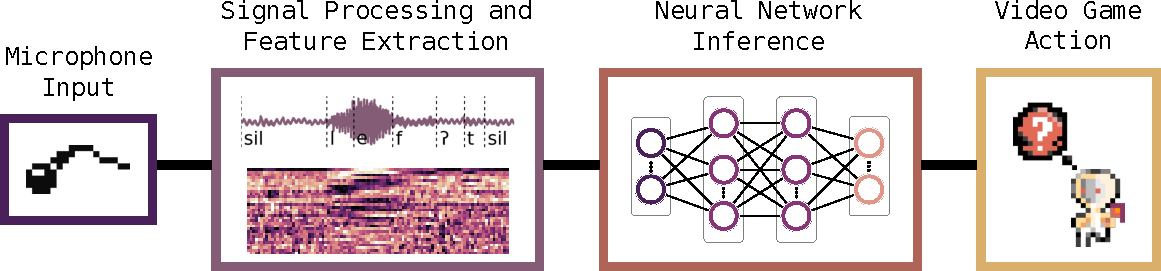
\includegraphics[width=0.95\textwidth]{./1_intro/figs/intro_kws.pdf}
  \caption{Simplified process of keyword spotting for video games.}
  \label{fig:intro_kws}
\end{figure}
\FloatBarrier
\noindent
From a semantic perspective, the controlling of game objects should be short, clear, and best done with single command words, which are referred in the following as \emph{speech commands}.
Single words can easier be identified in comparison to long sentences, for instance, it is easier to recognize the word \enquote{left} than the sentence \enquote{missile target on position x, y}.
Further, those speech commands can be classified through a KWS system composed of a neural network.
KWS is restricted by a limited set of selected keywords, referred to as \emph{vocabulary}.
For example, in terms of video games the set of keywords might have members like \enquote{left} or \enquote{right} to move an element within the game to either left or right, respectively.
The limited set of keywords is crucial to lower the complexity of the recognition task.
This is highly recommended since in practical KWS applications it is not necessary to cover all words of a natural language.
Especially in video games, where the game environment is constrained by rules, technical limits, and play-ability, KWS is perfectly suited as an alternative or augmented control system.
The size of the vocabulary and the selected words are two parameters that influence on the one hand the choice of the neural network architectures, which are evaluated on their computational efficiency and accuracy performance, and on the other hand the game interaction limited by the controls a player can choose from.
If the vocabulary of a KWS system would be too large, it would be harder to distinguish between two similar keywords.
In many KWS applications it is absolutely necessary to include labels for \emph{background noise}, \emph{silence}, and \emph{unknown words} in the vocabulary. 
This is especially interesting in \emph{wake word} applications, where a single keyword has to be detected over the previously mentioned labels representing either noise or any other possible word that a user might speak.
Also in video games those additional labels are useful to prevent the player from eliciting unintended commands accidentally through, for instance, loud background noise.
Therefore, a KWS system demands to be very accurate and fast in its classification of keywords.

Nowadays KWS systems are considered no science-fiction anymore, assisting consumers in everyday situations by rendering simple control tasks, such as triggering a photo release button on a \enquote{smartphone} with a single speech command.
Applications like this lead to more and more awareness of KWS and other speech recognition tasks in human society.
Unfortunately some consumer applications with integrated speech recognition systems cause some unpleasant side effects in data privacy and energy consumption due to an externally and extensive computational processing pipeline over corporate servers \cite{Tang2018}.
It is therefore important to design KWS systems that respect private user data and provide an efficient implementation in order to save energy consumption.

Video games are a potential application for KWS although until now, there exist only very few of them taking advantage of this special feature.
Reasons for that might be found in the history of video games itself, where players find themselves in fast paced arcade games and speech recognition is simply too slow.
Additionally the complexity of KWS and lack of training data are often two valid arguments for not considering the deployment of a KWS system into a video game.

The following two sections in this introduction will briefly explain the contributions of this thesis and give an overview of upcoming sections.
In summary, this thesis concentrates on KWS with neural networks trained by supervised learning on the speech command dataset \cite{Warden2018}.
The best suitable solutions for speech commands classification regarding video games are presented and evaluated with special interests in Convolutional Neural Networks (CNN), Generative Adversarial Neural Networks (GAN), and Wavenets.

% contributions
% --
% contributions

\section{Contributions}
A KWS system for video games requires fast response times.
Therefore, it is essential to reduce the classification time interval from the examples of the used speech commands dataset \cite{Warden2018SpeechCommands} from \SI{1}{\second} to at most \SI{500}{\milli\second}.
This can be achieved by determining the onset of the highest energy region within the speech signal by extracting the MFCCs and using the first cepstral coefficient as energy measure.
From the determined onset, the desired time interval is cut out of the original data example and used for further processing.

CNN models with low computational footprints, such as examined in \cite{Sainath2015KWS}, are the main evaluation subject within this thesis.
Besides a low computational footprint of the CNN models, the aim is to minimize the amount of neural network layers in order to reduce the complexity of the internal model structure.
The use of MFCC features as inputs to the CNN models required the conduction of experiments upon the number of cepstral coefficients and possible enhancements of MFCCs, such as delta, double delta, and energy features.
It is explained why a reduction of cepstral coefficients and sparing of enhancements are often preferred, especially for a computationally efficient solution.

A frame-based normalization (normalization regarding the time dimension) is introduced and performed on MFCCs to suite them better for visualization and GAN training.
Evaluation of the frame-based normalization is done in terms of recognition accuracy, and shift and noise invariance on conventional CNN models.
Moreover, the advantages and disadvantages of such a normalization technique are discussed.

Another large evaluation topic within this thesis is the application of GANs to generate new examples from the speech command dataset.
Note that GANs consist of a Generator (G) and Discriminator (D) network that are trained to compete against each other.
By applying frame-based normalization to the MFCC extracted speech command examples with the purpose to limit their values in the range of $[0, 1]$, G learns faster to produce fake images.
In the experiments it was found that when G and D were trained for too long, a noisy equilibrium state may emerge, where both networks generate random outputs of either fake images or decisions.
To solve this problem, a second loss term for G was added that measures the similarity of the generated samples to the input data by applying the cosine distance.
This helped to improve the generation of fake images and did not lead into noisy equilibrium states anymore.

Moreover, from the adversarial training of GANs, it is examined how the obtained weights can contribute to the performance of an equivalent CNN model with the same convolutional layer structures.
The transfer of the obtained weights (transfer learning) from either D or G is used in order to initialize the target CNN model for the KWS task.
The experiments show that the obtained weights of G can be very valuable when frame-based normalization is applied.

A completely different approach to the KWS task was the evaluation of a Wavenet \cite{Oord2016Wavenet} model for classification.
However, the initial assumption that without feature extraction a lower amount of computations is required in the application of an online system for video games, finally turned out to be wrong.
Wavenets have to run a huge amount of operations by processing each sample of the audio files from the dataset through dilated convolutional filters over many layers.
Furthermore, the classification accuracy of a reasonable sized Wavenet turned out to be very poor compared to the CNN approaches.
Nevertheless, this model with an extension for class predictions was evaluated and the obtained results are reported.

The integration of the KWS system into the video game is explained, where the KWS system consists of an online system for capturing the microphone input stream and a classification system that maps speech commands to certain actions within the game.

% overview
% --
% intro overview of thesis

\section{Overview}\label{sec:intro_overview}
After this introduction, \rsec{back} provides background information of the individual disciplines within this thesis, further some research questions are listed and give insight into problems of the KWS task for video games.
\rsec{prev} lists previous and related work, where a small history about neural networks is given and important works on neural network architectures are referenced, as well as works that influenced and motivated this thesis.
The audio signal processing part is located in \rsec{signal} and explains the extraction of meaningful features for speech recognition, such as MFCCs and an onset detection method for KWS.
The feature extraction and onset detection is guided with examples to visualize their properties.
In \rsec{nn} theory about neural networks in general, as well as the used neural networks architectures and the adversarial pre-training are described.
The experiments are presented in \rsec{exp} with a thorough observation of the dataset and a general listing of experimental details beforehand. 
Experiments were conducted on the feature selection of MFCCs, the adversarial pre-training, the Wavenet architecture and the final experiments running on the whole dataset.
\rsec{game} describes the integrated KWS system in detail and presents the game design of the deployed video game.
The thesis finishes with a conclusion and an outlook to future work in \rsec{conclusion}.


% --
% background section

\chapter{Background}\label{sec:back}
This section provides fundamental background information regarding KWS, neural networks and video games.
The KWS task is described mathematically to express the actual speech recognition problem.
Notes on neural networks explain common properties and terms in their application.
Research questions are listed and give a deeper insight in common challenges concerning the implementation of a KWS system into a video game.

% disciplines
% --
% Intro of keyword spotting

\section{The Keyword Spotting Task}\label{sec:intro_kws}
As described in \rsec{intro}, KWS is the task of classifying speech signals of spoken words to single keywords out of a set of keywords.
The set of keywords $S$, also referred to as vocabulary, can be defined by
\begin{equation}\label{eq:intro_kws_dict}
	S \coloneqq \{s_i \mid i = 0, 1, \dots, L\},
\end{equation}
where $s_i$ represents the $i$-th keyword of a set of $L$ keywords.
The task is to select the keyword closest to the spoken word from the user, denoted as target $t$.
The target does not necessarily have to be a member of the set of keywords $S$, in fact it can be any arbitrary word.
With the abstract formulation
\begin{equation}\label{eq:intro_kws_task}
	\hat{s} = \underset{s_i \in S}{\arg \min} \, \mathcal{D}(t, s_i),
\end{equation}
the most probable keyword $\hat{s}$ can be predicted, where $\mathcal{D}$ is some kind of distance measure between two words.
The formulation in \req{intro_kws_task} is merely semantic but KWS in computer systems have to cope with various transformations of raw input samples $\bm{x} \in \R^n$ of audio data with a total number of $n$ samples.
An inference from audio data to output class probabilities $\bm{y} \in \R^L$ can, for example, be achieved by the use of a neural network containing a softmax function at its last layer (transforming the output of the last layer to probability values).
The most probable keyword can therefore be picked by
\begin{equation}\label{eq:intro_kws_class}
	\hat{s} = \{s_i \mid \underset{i = 0, 1, \dots, L}{\arg \max} \, y_i\},
\end{equation}
where the index $i$ of the output class probability $y_i$ corresponds to the intended keyword $s_i$ in the vocabulary.

In comparison to full Automatic Speech Recognition (ASR), where whole sentences need to be identified, KWS operates merely on the word level.
Therefore, KWS is slightly easier to deploy and less complex than ASR.
Conversely, KWS systems have to run very energy efficiently on low-resource devices, such as mobile phones, and provide immediate and accurate responses to the users.
A good elaboration on the requirements of KWS systems can be found in the motivation section of \cite{Warden2018}.
% --
% Intro to neural networks

\section{Notes on Neural Networks}\label{sec:intro_nn}
Neural networks enable computers to automatically learn from data to be able to solve tasks, such as pattern recognition in images or audio.
The \emph{training} of a neural network with a specific dataset, is the learning process of all parameters within its architecture.
The examples or samples from the input data can be paired with annotations, denoted as \emph{labels} or \emph{classes}.
If the label information of each example is used during the training of a machine learning system, such as a neural network, it is called \emph{supervised learning} otherwise it is called \emph{unsupervised learning}.
Yet supervised learning is more commonly applied.
\emph{Inference} is simply the forward pass of input data samples through an already trained network to output their estimated class labels.

The main advantage of neural networks is that they are able to cope with large amounts of input variables per data example.
Considering a raw waveform file of merely \SI{1}{s} time duration, sampled with \SI{16}{\kilo\hertz} would give an input size of 16000 features.
This huge amount of input features is even difficult for neural networks to learn from with restricted computational resources and usually a feature extraction stage is placed in between to reduce the input dimension.
For instance, the computation of MFCCs with 12 coefficients and a time duration of \SI{0.5}{s} with a time shift of \SI{10}{\milli\second} reduces the input feature size dramatically to $12 \times 50 = 600$, which is still a high number of input features but much more affordable and faster to train.

Neural networks are able to learn own feature representations, selection and interpretation, rather than using hand-crafted ones done by humans with expertise in the research field.
Note that hand-crafting features of complex recognition tasks is in most cases not even possible or extremely cumbersome.
So researchers prefer neural networks because of their easy deployment scheme and state of the art performances.
Furthermore, it enables everyone capable of using neural network tools to create solutions to rather complex problems, given there is enough data and processing power available.
This causes that elaborate feature extraction stages become less relevant to the users, which may lead to some extend into the ignorance of the classification problem and more \enquote{try and error} approaches of different neural network architectures and training parameters.

The energy consumption required to train Deep Neural Networks (DNN) with many parameters on a huge training dataset, shall not be forgotten, especially in times of climatic change.
Reusing pre-trained weights from renowned network architectures is a good manner to reduce energy consumption in finding an optimal classifier for an already widely examined classification task.
The re-usability of pre-trained weights is often named as \emph{transfer learning}, where a small comprehension on it can be found in \cite{TransferLearning}.

Nevertheless, the potential of neural networks in research are vast.
The observation on how the learning from data is done and what recognition patterns are obtained after training, might allow researchers and experts to better understand the problem or gain a different viewpoint on it.
Especially the use of CNNs allows researchers to visualize the learned filters and interpret their results.
A very interesting example of investigating learned CNN filters is shown by Zeiler et al. \cite{Zeiler2013}.
Other exciting subjects in research are generative models, such as GANs \cite{Goodfellow2014}, which are able to create convincing samples from the learned data distribution.

Neural network architectures for speech recognition are a little bit different from image recognition, mainly because of the sequential nature of time signals.
However, if time signals are restricted in time, which implies that they are limited to a fixed number of samples, and frequency features are extracted over that time span, then speech signals can be represented in 2D space (frequency and time) and classified like images.
That suggests that CNNs are reasonable network architectures for speech as well.
Another potential architecture for audio signals is the Wavenet \cite{Oord2016} because of its ability to process raw audio data.
% --
% video games with speech commands

\section{Video Games with Key Word Spotting}\label{sec:intro_games}
Video games with KWS or any speech input are rarely seen gems in the gaming industry, though it is an exciting and immersive way to interact.
Technically the voice of the player has to be recorded by a microphone, therefore one additional requirement to play the video game is to own a microphone, which however does not need to be high-end.
The input stream of a microphone can be processed through an online or real-time system to extract the input features for the classification system.
The classification system, such as a neural network, is supposed to infer the input information to the intended action within the game.

The processing scheme is easy to define, but not that easy to implement compared to other more hardware based input channels, such as pressing buttons on a keyboard.
Also speech input is very slow compared to hardware input, where players are able to interact within tens of milliseconds (the input lag of gaming controllers should ideally be under \SI{50}{\milli\second}).
This fast response time is not possible with speech, where the player has to physically form a waveform representing the action in the game.
Further the waveform captured from the online system has to be pre-processed, feature extracted and classified to the best estimation of all the available key words in the game's vocabulary.
Concluding this, a good estimate to create and process a speech input should ideally be under one second, the less the better for the playing experience.

Another important consideration has to be made upon the size of the vocabulary.
A high number of key words will increase the chance of confusion and a small number of key words restrict the possible actions a player can choose from.
The possibility to create separate classifiers with different sets of smaller vocabularies of speech commands arises, depending on which commands the player needs in the actual scene of the video game.
For instance, if the player is in a dialogue with a Non Player Character (NPC), it makes sense to reduce the vocabulary to only \{\enquote{yes}, \enquote{no}\}, if those are the only actions to choose from.

The use of labels for background noise, silence and unknown words depends on the game and how the classification process is activated.
If the assumption is made that a player chooses only from the key words in the dictionary, then the label of unknown words is not necessarily required.
However the unknown label would be very interesting if key words are not that common to a player, such as words from a different language or fantasy words.
The unknown label will therefore motivate the player to correctly pronounce the word itself, which could be also used in language learning games.
The labels for background noise and silence are useful in the case of initializing the classification process by the energy value of the input stream of the microphone.
A small impact on the microphone or loud background sound can therefore elicit an unwanted command within the game, if those labels do not exist in the vocabulary.

In KWS video games, players have to act with their voice, which is in some situations not appropriate or annoying, for instance playing a video game in a public transport and shouting into ones mobile phone or laptop might anger other passengers.
Also the slowness of KWS and many other reasons makes it not suitable for every game type.
Luckily the existing types and genres in video games are vast and there might be one or two game ideas where KWS makes a game outstanding, creative and refreshing.
Potential of KWS lies without doubt in the domain of Virtual Reality (VR) and Augmented Reality (AR) applications and games.
In VR the player wears a Head Mounted Device (HMD), where most recent consumer devices have already incorporated a microphone, most commonly used for online chat, but also ready to adopt for KWS.
To increase immersion in VR even further, a KWS systems can be very valuable.

% research questions
% --
% research questions

\section{Research Questions for this Thesis}\label{sec:intro_rq}
This section formulates relevant research questions regarding KWS in video games.
Those research questions can be split into 3 parts:
\begin{enumerate}[label={Q.\arabic*)}, leftmargin=1.4cm]
  \item Signal processing and feature extraction of speech signals.
  \item Neural network training and classification for KWS.
  \item Video games with KWS.
\end{enumerate}
Note that the terms \enquote{key word} and \enquote{speech command} are often named interchangeably because speech commands are used as key words in the KWS system.
Not all research questions can be answered within the scope of this thesis.
Nevertheless, those questions can be asked and some solution concepts discussed.


% --
% signal

\subsection{Signal Processing and Feature Extraction Research Questions}\label{sec:intro_rq_signal}
Acquiring meaningful features from speech signals is essential for neural networks to operate on. 
The features are extracted from raw audio samples of a microphone input stream in a specific time interval.
Those retrieved features are further input to a neural network for the classification of speech commands.
The following Questions arise here:
\begin{enumerate}[label={Q.1.\alph*)}, leftmargin=1.75cm]
  \item Which time interval should be captured to represent a speech command?\label{it:q1-a}
  \item Does the signal processing have to be invariant to background noise and especially to game sounds?\label{it:q1-b}
  \item What are meaningful features for speech recognition?\label{it:q1-c}
\end{enumerate}
\noindent
\textbf{Question \ref{it:q1-a}:} 
The time required to fully pronounce a speech command is not fixed and varies from speaker to speaker, depending also on the intended prolongation a speaker adds to the word.
In practical applications however, a fixed time interval for a single speech command is convenient.
By restricting the time duration of the key words, the speaker has to pronounce the words within this time span.
For example, if a speaker pronounces the word \enquote{left} and requires a time duration of \SI{1}{\second}, hardly all is captured if the time interval is restricted to merely \SI{500}{\milli\second}.
Whether this \SI{500}{\milli\second} is sufficient for a correct classification, is subject for evaluation.
In the application of a video game, the user should preferably speak the commands with a short time duration, so that the game can respond fast.
Problems might occur if the speech commands are spoken repeatedly and very hasty, so that the time interval of consecutive commands overlap each other.
Ideally the time interval to represent a speech command would be flexible but this more difficult to implement than a fixed time interval.

\textbf{Question \ref{it:q1-b}:}
Usually the presence of low background noise should not be a problem for neural networks trained on a large enough data set. 
The game sounds might present a more difficult problem, when turned up too loud without the use of headphones. 
Therefore, the microphone will not only capture the voice of a speaker but also a fair amount of game sounds. 
This problem seems to be theoretically solvable as the shape of the nuisance is known and the amount of game sound in the audio stream could be attenuated sufficiently.
In practice this might be hard to solve without critically disturbing the signal of interest.
A solution to this problem would probably take too much time and effort and is therefore not evaluated within this thesis. 
However, playing a video game without game sound is unsatisfying and it would be a great contribution to tackle this problem in future work.

\textbf{Question \ref{it:q1-c}:} 
The determination of meaningful features for speech signals is a classical problem in speech recognition.
The essential composition of a word may help to understand the problematic better.
A word is a sequential combination of either vowels, such as \enquote{a} and \enquote{e}, or consonants \enquote{k}, \enquote{l}, with a certain length. 
In linguistics for instance, it is possible to distinguish vowels with frequency peaks in a spectrogram, where a spectrogram is the magnitude squared of the frequency response of small time chunks over the time duration of a signal.
However, due to many different factors in voice generation involved in speakers, such as age, gender, nationality and physiology of the vocal tract, there is a huge variance in the pronunciation of words from different persons, which increases the difficulty of the problem.
A very common approach is to use MFCCs as features for speech recognition tasks.
Why MFCCs present good features for speech is described in detail in \rsec{signal_mfcc}.


% --
% neural networks

\subsection{Neural Network Implementation Research Questions}\label{sec:intro_rq_nn}
Neural networks for video games should ideally be very efficient and provide accurate classifications of input features.
The vocabulary in a KWS task has to be specified for the individual game and chosen from all class labels available in the dataset.
Each key word of the vocabulary is presented by one output node of the neural network architecture.
Following Questions can be asked in general:
\begin{enumerate}[label={Q.2.\alph*)}, leftmargin=1.75cm]
  \item Is there an appropriate dataset suited for KWS video games and with sufficient diversity available?\label{it:q2-a}
  \item What happens if an input feature represents a spoken word, which is not in the vocabulary (unknown key word) and how should this exception be handled?\label{it:q2-b}
  \item What is the best neural network architecture regarding classification accuracy and energy efficiency?\label{it:q2-c}
  \begin{enumerate}[label=(\roman*)]
    \item Can adversarial networks improve generalization?
    \item Are Wavenets a solution to this task?
  \end{enumerate}
\end{enumerate}
\noindent
\textbf{Question \ref{it:q2-a}:} 
The availability of a dataset for KWS video games can be answered right away, as there exists a speech commands dataset \cite{Warden2018} with enough and diverse data.
The dataset consist of 35 labels and contains commands for movement and numbers.
Further, it includes randomly selected words like \enquote{marvin} or \enquote{bird} intended to represent \emph{unknown} words for the KWS system.
It has to be noted that not every game idea can be realized with a restricted vocabulary.
Nevertheless, with commands for movement like \enquote{left} or \enquote{go} it is possible to move objects within a game and this can already be used for many game mechanics.
An aspect regarding efficiency, is to restrict the amount of key words in the vocabulary as much as possible such that a cheaper neural network architecture can be deployed, which of course should still be sufficiently good in its classification accuracy.

\textbf{Question \ref{it:q2-b}:} 
Without doubt, players will try out words that are not in the vocabulary (denoted as \emph{unknown} key words) and observe the response of the video game.
The ideal response would be to shown an indication to the player that the word is not present in the vocabulary. 
Nevertheless, it might happen that the similarity of a unknown key word is too close to a key word and an unintended action is triggered in the game. 
At the same time the neural network should not classify key words as unknown key words to ensure a satisfying game experience.
It is better to rely on that players are using key words for most of the time so that they are preferred over unknown key words.

\textbf{Question \ref{it:q2-c}:}
In the ideal case, video games with KWS do not slow down during the inference process of unknown input data.
The restriction of the amount of computations and time for the classification of key words is given by the minimum Frames Per Second (FPS) a video game is perceived as fluent.
That requires the FPS to not fall under a certain limit (usually 30 FPS in video games), otherwise the fluidity of the game is not guaranteed.
Several different neural network approaches with a low computational footprint must therefore be tested and compared against each other regarding classification rate and energy efficiency.
The transfer of weights from GANs is an interesting approach to evaluate whether the trained parameters are also useful for pure classification tasks in CNNs.
Wavenets have the advantage that they do not need a feature extraction stage but it is questionable whether the network design achieves a reasonable computational footprint.


% --
% video games

\subsection{Video Games with KWS Research Questions}\label{sec:intro_rq_games}
Video games that use KWS can create a unique playing experience but must face certain challenges.
Following questions can be stated:
\begin{enumerate}[label={Q.3.\alph*)}, leftmargin=1.75cm]
  \item How should the onset of a key word be detected, so to reduce computations?\label{it:q3-a}
  \item What is the added value of KWS in the gaming experience of players?\label{it:q3-b}
  \item What do game developers have to consider, when designing a game with KWS?\label{it:q3-c}
\end{enumerate}
\noindent
\textbf{Question \ref{it:q3-a}:} 
It is crucial to reduce computations in a video game in order to keep it running fluently during high performance peaks.
Also the unnecessary processing of meaningless input data should be avoided as much as possible.
Ideally the key word classification is activated, when there is actually a speech command present, which however is not always trivial.
One possibility to indicate the onset of a key word is to perform the relatively efficient calculation of an energy value within a certain time interval of the raw input data stream and have a simple threshold value decide, whether a speech command is available. 
To avoid the consecutive triggering of onsets at each energy measure, the microphone and amplifier noise floor and the background sound (including the game sound) have to be less energy intensive than the speech signal obtained from the player.
Another approach similar to the push and talk principle, would be to indicate the onset of a key word with the click of a certain button on the keyboard.
The player is therefore able to control the exact onset of a key word and its length but requires an additional hardware based input channel.

\textbf{Question \ref{it:q3-b}:}
In certain video game scenarios, speech commands can be useful, interesting and enhancing for the gaming experience, in others they might even disturb the game play or even spoil it completely.
It cannot be generally stated whether it is worth to deploy a KWS system into a game, this depends on the game it is intended for.
As already noted in \rsec{intro_games}, KWS might be a great augmented control system for special kind of games to increase the immersion experience, especially for VR applications.
Also language learning games are an interesting application but usually require a huge vocabulary and therefore a phoneme based ASR system would be the better choice.

\textbf{Question \ref{it:q3-c}:}
Apart from the technical requirements involved in KWS systems, also the general game design with KWS has to be considered.
It certainly can be stated that KWS systems are not always reliable and therefore a main game mechanic solely based on it is not always preferred.
Furthermore, the time lag required to process speech commands to actual actions within the game should not be ignored.
The player should for one get immediate and accurate feedback from the game and on the other hand be challenged while playing so that the game experience does not get frustrating or tiresome.
Using speech commands consecutively, can also be very exhausting for the player and maybe it is better to use KWS only in special situations within the game.
Generally it can be stated that a game developer has to design a KWS game with care.
% --
% previous and related work

\chapter{Previous and Related Work}\label{sec:prev}
This section presents previous and related work on which this thesis was built, motivated, and influenced upon.
The work can be separated into work on audio features, neural networks, KWS with neural networks, and video games with KWS.

% features
% --
% prev features

\section{Work on Audio Features for Speech Recognition}\label{sec:prev_features}
The feature extraction of audio signals is crucial for an efficient data compression and extraction of relevant information, which make the extracted features suitable for further processing and classification tasks.
Not all audio signals should be handled in the same manner, as for instance, speech signals are very different from musical signals.
Music has its significant features in rhythm and pitch patterns, while speech does not specifically depend on those.
Speech can be spoken in different duration and pitch, depending on the speaker and the situation.
Therefore, speech signals are usually extracted to \emph{low-level features} that do not emphasize specific structures of duration and pitch.

One of the most popular low-level features for speech recognition are the MFCCs, introduced by \cite{Mermelstein1980} in 1980.
MFCCs are motivated by the physiological human hearing system using equidistant Mel-frequency bands and are described in detail in \rsec{signal_mfcc}.
Another popular low-level feature similar to MFCCs are Perceptual Linear Prediction (PLP) features introduced by \cite{Hermansky1987}.
PLPs have not been evaluated in this thesis yet it would have been interesting to compare their performance to MFCCs in the KWS task of speech commands.
A well prepared summary and comparison between PLP and MFCC can be found in \cite{Hoenig2005}.

Recently raw audio samples can be used directly as input features to some special kind of neural networks, such as the Wavenet. 
However, the size of the input features is huge and there is no frequency correlation between the features except from the waveform they present.

% neural networks
% --
% prev neural networks basics

\section{History and Work on Neural Networks}\label{sec:prev_nn}
Over the years, many different neural network architectures emerged from different research fields.
Historical remarks on neural networks in general are presented, as well as a brief overview upon some basic and modern architectures, that are meaningful in regards to this thesis.


% --
% prev history

\subsection{Historical Remarks on Neural Networks}\label{sec:prev_nn_history}
The first step towards computational neural networks, as we know them today, was the introduction of the so called \enquote{Perceptron} by Rosenblatt in the year 1958 \cite{Rosenblatt1958}. 
The idea of the Perceptron emerged from physiologists, trying to model a physiological neural network in computational terms. 
This first model was based on the information processing of the retina (input nodes), which passes through several physiological neural networks (hidden nodes) and finally elicit an action or decision (output nodes).
Publishing his work and implementing those ideas in an actual computer system (at those time computers were huge boxes), Rosenblatt kicked of the domain of computational learning systems.
The race of finding best neural network architectures for specific regression or classification tasks had begun.

Another big advance in the history of neural networks, was the introduction of a very famous learning algorithm known as \enquote{backpropagation}, evolved by several authors at the same time \cite{LeCun1986} and \cite{Rumelhart1986} in the late 80s. 
Even nowadays, 35 years after introducing backpropagation, it is still the \emph{de facto} standard in training neural networks.
Nowadays backpropagation is implemented in every machine learning framework for neural networks as its core element.
Such frameworks are for instance \texttt{Pytorch} \cite{Pytorch} or \texttt{Tensorflow} \cite{Tensorflow} and of course many others, handling the gradient calculation (automatic differentiation) and backpropagation algorithm of those gradients in the background.

The neural networks reputation during the time until now, was not always seen that splendid.
The general problem of handling overfitting (prevent networks from learning data samples by heart) and generalize better on unseen data, is still an open issue in many applications.
Some mathematicians working in the field of statistical methods in learning theory for pattern recognition, regard neural networks as being not meaningful in the advance of learning theory, such as one quote from \cite{Vapnik1995} of Vapnik's book in 1995 about natural learning theory:

\begin{quote}
...In spite of important achievements in some specific applications using neural networks, the theoretical results obtained did not contribute much to general learning theory...
\end{quote}

This quote is a bit tough, but unfortunately true in some sense. 
The complexity of neural networks with many layers, makes the tracing of the learning process very difficult.
No concrete formulas, apart from the calculation of gradients, can exactly explain what neural networks are actually learning.

Therefore on one side there were the classical statistical learning methods, the most famous one called Support Vector Machines (SVM) \cite{Cortes1995} and one the other side there were neural network approaches.
Over a long period of time SVMs were preferred over neural networks, because they were better understood with a profound mathematical background and achieved state of the art performances with sophisticated feature extraction stages.
Not until 2012, neural networks gained more popularity again by scoring new benchmarks in image classification tasks with one famous paper \cite{Krizhevsky2012}, where the previous benchmark of the best statistical method was bested by a significant score.
Deep Learning was the new key to success, with network architecture consisting of many layers and large amounts of parameters to train.
Also in audio and language processing tasks, such as KWS, ASR and Natural Language Processing (NLP), the famous Hidden Markov Models (HMM) and other statistical methods get more and more replaced by neural networks.


% --
% convolutional nets

\subsection{Convolutional Neural Networks}\label{sec:prev_nn_cnn}
CNNs are a special type of neural networks consisting of convolutional layers, that are able to incorporate spatial information from the input data, with the application of convolutional filters to create so called feature maps as outputs.
Spatial information is very important in images, where neighboring pixels are correlated to each other.
The same holds for audio, but only in one dimension (time).
Convolutional filters are very commonly applied in image processing tasks, such as denoising and other enhancements.
In audio processing a classical application of convolutional filters, is a simple average filter of the signals energy, to determine onsets like the start of a speech signal.

Still it took relatively long until convolutional filters were a common and a widely used asset in neural network architectures.
The general concepts of CNNs producing feature maps and weight sharing through convolutional filters, were examined by LeCun et al. on handwritten postal codes in 1989 \cite{LeCun1989_Generalization}.
Further research and experiments on the famous MNIST dataset of handwritten digits, were done in the late 90s \cite{LeCun1998} and asserted the success of CNNs.
A classical convolutional layer in CNNs usually consists of multiple convolutional filters with trainable weights and an additive bias term (optional) per filter, followed by a non-linear activation function.
More details about CNNs an its convolutional layers and how they transform input images to feature maps are presented in \rsec{nn_theory_cnn}.


% --
% recurrent neural networks

\subsection{Recurrent Neural Networks}\label{sec:prev_nn_rnn}
Recurrent Neural Networks (RNN) are a type of neural networks, that are using feedback loops from the output of each node back to its input.
With those feedback loops it is possible to accumulate information of sequential input data and might overcome the restriction of fixed sized inputs.
However RNNs are known to be hard to train, because of the well known exploding or vanishing gradients problem.
This problem can be solved by using so called Long Short Time Memory (LSTM), that are incorporating gates for the information storage in each cell. 
However the LSTM cell also increases the amount of parameters to train and backpropagation over a large amount of time steps is computationally intensive.

Through their design to capture sequential data, RNNs are commonly used in speech recognition tasks.
However RNNs are not subject in this thesis, the interested reader is referred to the summary presented in \cite{Staudenmeyer2019} including further references upon the mentioned problems and architecture types.


% --
% wavenets

\subsection{Wavenets}\label{sec:prev_nn_wavenet}
Processing raw audio data as inputs to neural networks seemed to be difficult for a long time, mainly due to the huge amount of input dimensions.
Recently neural network architectures emerged with the ability to process raw audio samples.
One very prominent architecture, originally intended for natural speech generation, is the so called \emph{Wavenets} \cite{Oord2016}.

With the application of \emph{dilated convolution} and a quantization of the audio sample values, Wavenets can afford to process a huge amount of input dimensions and at the same time extract relevant information.
The implementation of Wavenets should be more efficient compared to LSTMs, such as the quote from \cite{Oord2016} states:
\begin{quote}
  ...With WaveNets we have shown that layers of dilated convolutions allow the receptive field to grow longer in a much cheaper way than using LSTM units...
\end{quote}
A classification task of musical pieces to corresponding music artists in \cite{Zhang2020}, was done with a Wavenet model.
However it is to mention, that there are not many papers about classification tasks with Wavenets and it is questionable, whether Wavenets are suited for the KWS task of speech commands.


% --
% adversarial nets

\subsection{Generative Adversarial Neural Networks}\label{sec:prev_nn_adv}
GANs emerged from Goodfellow et al. in 2014 \cite{Goodfellow2014} and was initially motivated by Game Theory of a two player zero-sum game with the Min-Max-Theorem as solution concept \cite{VonNeumann1944}.
The game in terms of GANs is, that two neural networks try to outperform the other in an adversary task, where the task hereby is the generation of fake images by one network, denoted as Generator (G) and the detection or discrimination of real and fake images by the other network, denoted as Discriminator (D).
In \cite{Radford2016} some practical guidelines for designing and training deep GAN architectures are shown with the Deep Convolutional Generative Adversarial Network (DCGAN) model.
DCGANs however consider only images and not speech signals, but they were the first starting point for developing GANs in this thesis.

The G network, has to perform a so called \emph{transposed convolution}, \emph{up-convolution} or \emph{de-convolution} for upsampling the low-dimensional image to the desired output dimensions of the real sample images from a dataset.
The transposed convolution and some problems regarding GANs are described in \cite{Durall2020}.

GANs are not the only application of adversarial neural networks, in \cite{Oezdenizci2020} it is shown how an adversarial network improves generalization over invariance of subject specific samples from Electroencephalogram (EEG) data.
The adversarial network in this paper is connected to a convolutional encoder network, which is also input to a classifier network.
The update of the encoder network is therefore done via the adversarial network and the classifier network at the same time and specified in a collective loss function.

In this thesis, the concept of GANs is used for pre-training weights to improve generalization and performance in a CNN network.

% KWS for speech commands
% --
% prev key word spotting

\section{Key Word Spotting with Neural Networks}\label{sec:prev_kws}
\thesisStateRevised
Some important works regarding KWS with neural networks are presented here. 
The aspect of energy efficients is very important within this thesis, because of the deployment of a KWS system in a video game.
Further the neural network architectures evaluated in this thesis are trained and tested on an already profoundly examined speech command dataset \cite{Warden2018}.
Actual benchmarks are provided on classification accuracies from different neural network approaches.


% --
% energy efficient

\subsection{Energy efficient solutions}
In video games the processing and classification of speech commands has to run in real-time and therefore a low computational footprint is needed for the deployment of neural networks in this task.
One of the most famous papers on low computational footprint regarding KWS systems is from Sainath et al. in 2015 \cite{Sainath2015}.
Two neural network architectures are chosen from this paper, one is a traditional CNN network for comparison and the other is a limited multipliers network with a CNN striding only in the frequency axis.
Both networks are described in detail in \rsec{nn_arch}.

A deployment of a KWS system on microcontrollers is examined in \cite{Zhang2017}.
Different neural network architectures were evaluated regarding their memory usage and operations per inference.
The work showed that 32-bit to 8-bit quantization does not reduce the classification accuracy and that the depthwise separable CNN (DS-CNN) was the best choice with regards to limited amounts of memory and operations compared to the other evaluated networks.

Another highly optimized resource efficient Deep Neural Network (DNN) based on CNNs obtained with a Neural Architecture Search (NAS) is described by \cite{Peter2020}.
This work also showed that a 1-bit quantization of the weights performs nearly as good as the 8-bit quantization, which decreases the memory usage even further.


% --
% benchmark

\subsection{Benchmark Networks for this thesis}\label{sec:prev_kws_benchmark}
First it is to mention that the speech command dataset \cite{Warden2018} exists in two versions \texttt{v0.01} and \texttt{v0.02} consisting of raw audio data in the \texttt{.wav} format and there is no pre-processing or feature extraction done beforehand.
Also it is up to the users for which labels are to be selected.
The main idea however is to choose the \emph{core words} as classification labels and add an \enquote{unknown} label for the \emph{auxiliary words}.
Also a separate noise or \enquote{silence} label can be added from given noise data files.
In most papers the core words were \{\enquote{left},  \enquote{right}, \enquote{up}, \enquote{down}, \enquote{go}\, \enquote{stop}, \enquote{yes}, \enquote{no}, \enquote{on}, \enquote{off}\} and two label for \enquote{silence} and \enquote{unknown} (all other words) used for comparison to previous papers.
This constellation of selected key words is referred here as \texttt{L12}, the speech command dataset version is referenced with \texttt{V1} or \texttt{V2}.
More details about the dataset is presented in \rsec{exp_dataset}.

One benchmark is hold by \cite{Berg2021} introducing a Key Word Transformer (KWT) network, which performs accuracy scores of almost 100\%.
A good overview of actual benchmark scores regarding the speech command dataset is given in \cite{PaperswithcodeKWS}.

All benchmark scores from the referenced works in this section are shown in \rtab{prev_kws_bench}.
\begin{table}[ht!]
\small
\begin{center}
\caption{Benchmark on the speech commands dataset.}
\begin{tabular}{ M{4cm} M{2cm} M{2cm} M{2.5cm} }
\toprule
\multirow{2}{*}{\centering\textbf{Model Name}} & \multicolumn{2}{c}{\textbf{Accuracy}} & \multirow{2}{*}{\centering\textbf{Operations}} \\
& V1-L12 & V2-L12 & \\
\midrule
DS-CNN-S \cite{Zhang2017} & 94.4 & - & \SI{5.4}{\mega\ops} \\
DNN-MFCC20 \cite{Peter2020} & 96.3 & - & \SI{27.1}{\mega\ops}\\
KWT-3 \cite{Berg2021} & 97.2 & 98.5 & ? \\
\bottomrule
\label{tab:prev_kws_bench}
\end{tabular}
\end{center}
\vspace{-4mm}
\end{table}
\FloatBarrier
\noindent
Note that this scores are achieved by very sophisticated neural network architectures incorporating many layers.
It is very hard to achieve the same performance as presented in those papers.

% games
% --
% prev games

\section{Video Games with Key Word Spotting}\label{sec:prev_kws_games}
Very few papers are tackling KWS specifically tied to video games and most research is conducted on gaining the best accuracies on datasets and setting new benchmark scores on them.
Nevertheless a research paper found, was that of a multiplayer video game intended for children presented in \cite{Harshavardhan2015}, which evaluates challenges when children are playing video games, such as repetitive and overlapping commanding.
On the other hand there are plenty of real world applications for KWS and ASR using available toolkits.
One very powerful tool for speech commanding widely used for video games is \texttt{VoiceAttack} running on \enquote{Windows Speech Recognition} \cite{Xiong2017}.
With \texttt{VoiceAttack} it is possible to specify own voice commands that are triggering combinations of keyboard clicks and therefore can be used to elicit actions in video games.
The applications are vast and flexible and can be applied in any game by running the program in the background.
An actual video game with integrated speech commanding ability, running with the \texttt{PocketSphinx} \cite{Huggins2006} speech recognition system, is \texttt{In Verbis Virtus}, where the players are able to cast spells by speaking out fantasy words after clicking an activation button as onset indication.
% --
% signal processing

\chapter{Signal Processing and Feature Extraction}\label{sec:signal}
This section describes the extraction of meaningful features for speech recognition from raw audio waveform files.
The feature extraction stage compresses and reduces the dimension of input data, hence it decreases computational effort for subsequent neural networks operating on the extracted features.
Moreover, this section discusses and explains properties of raw audio waveforms and the extraction to spectral features, such as the computation of a spectrogram. 
The extraction of MFCC features includes the computation of their enhancements, such as deltas and energy features.
Further, a normalization technique is described that improves the visualization of MFCCs.
Finally, this section outlines an efficient onset detection method that determines the start of keywords in speech signals.

% --
% raw audio

\section{Raw Audio Waveforms}\label{sec:signal_raw}
\thesisStateRevised
\thesisStateNew
Physical acoustic waves can be recorded by microphones, translating mechanical vibrations to electrical signals. 
Those electrical signals are further stored in \emph{waveform files} or \emph{audio files} with a specific audio format, for example the \texttt{.wav} format.
Apart from any compression technique the most important storage details are the bit resolution, for example \SI{24}{\bit} floating point and the sample rate $f_s$. 
The sample rate defines, which frequency range of a continuous acoustic waveform can be stored in a discrete representation.
This is restricted by the Nyquist-Shannon sampling theorem, where the maximal frequency of the signal $f_{x_{max}}$ should not exceed the half of the sampling frequency: 
\begin{equation}\label{eq:signal_raw_nyquist}
  f_{x_{max}} < \frac{f_s}{2}
\end{equation}
to prevent aliasing effects.
That is the reason, why the compact disc (CD) format has a sampling frequency of \SI{44.1}{\kilo\hertz} resulting in a maximum signal frequency of \SI{22.05}{\kilo\hertz}, using the fact that humans do not hear above \SI{20}{\kilo\hertz} frequencies.
However it is also possible to go far beyond those \SI{44.1}{\kilo\hertz}, for instance used in telephone systems, where the sampling rate is \SI{8}{\kilo\hertz}.
It is possible to reduce the sampling rate, because voice does not need such a high sampling frequency to have sufficient quality and being understandable.
Music on the other hand requires a high sampling frequency for being enjoyable to listen to.

With the sampling frequency known, a discrete time signal of an audio recording $\bm{x} \in \R^n$ can be expressed in vector notation:
\begin{equation}\label{eq:signal_raw_x}
  \bm{x} = [x_1, x_2, \dots, x_n]^T
\end{equation}
with a total number of $n$ samples.
The recorded audio files provided in the speech command dataset \cite{Warden2018} used for the experiments in \rsec{exp}, are sampled with a sampling rate of \SI{16}{\kilo\hertz}, which is enough for human speech signals.
Further those recordings usually have a time duration of \SI{1}{\second}, apart from some individual shorter files.

For evaluation and visualization purpose, the author of this thesis recorded his own examples of the speech commands \{\enquote{left}, \enquote{right}, \enquote{up}, \enquote{down}, \enquote{go}\} with a simple consumer lavalier microphone.
Those showcase examples, shown in \rfig{signal_raw_showcase} in raw audio format, will be used to illustrate the whole feature extraction process in the following sections.
\begin{figure}[!ht]
  \centering
    \subfigure[left]{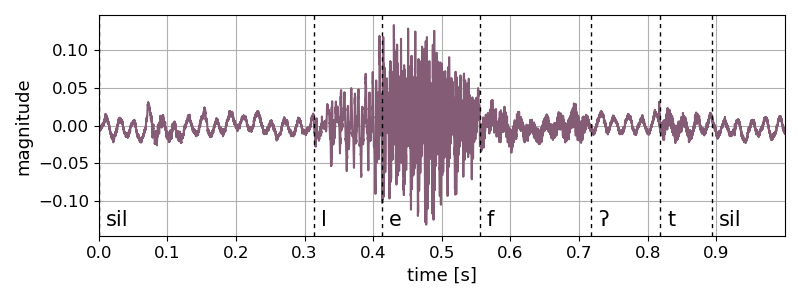
\includegraphics[width=0.45\textwidth]{./3_signal/figs/signal_raw_showcase_left0}}
    \subfigure[right]{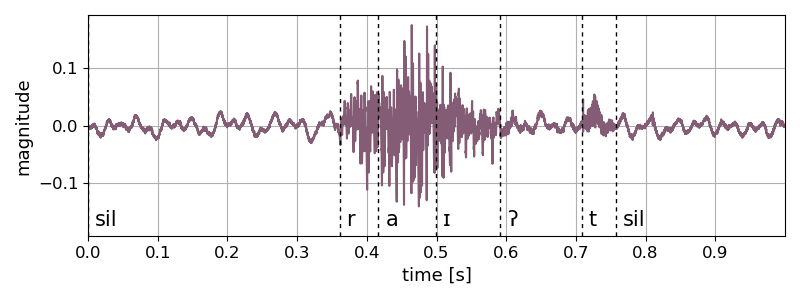
\includegraphics[width=0.45\textwidth]{./3_signal/figs/signal_raw_showcase_right0}}
    \subfigure[up]{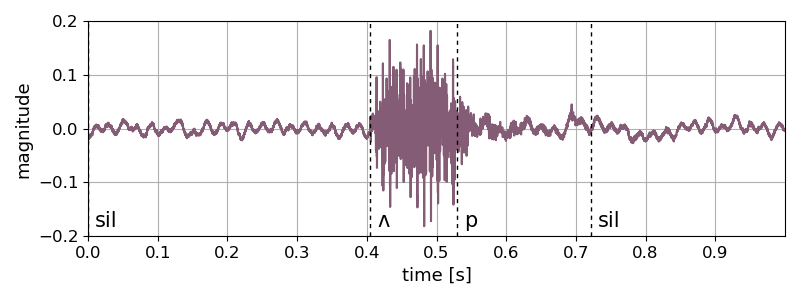
\includegraphics[width=0.45\textwidth]{./3_signal/figs/signal_raw_showcase_up0}}
    \subfigure[down]{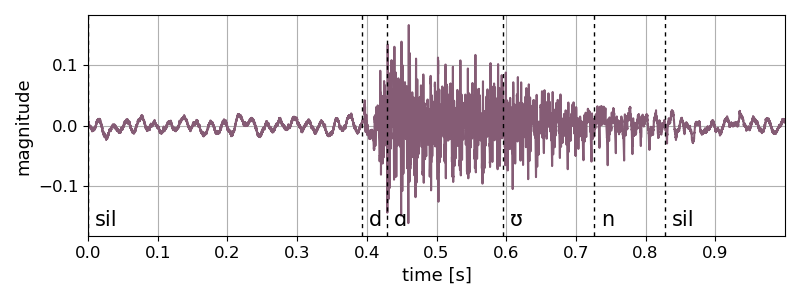
\includegraphics[width=0.45\textwidth]{./3_signal/figs/signal_raw_showcase_down0}}
    \subfigure[go]{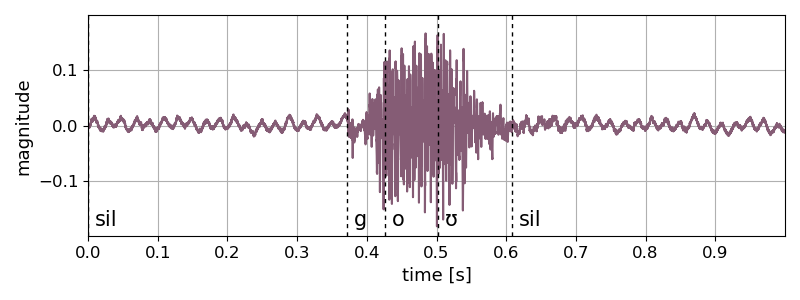
\includegraphics[width=0.45\textwidth]{./3_signal/figs/signal_raw_showcase_go0}}
  \caption{Self recorded raw audio waveform examples with phoneme onsets marked as vertical dashed lines.}
  \label{fig:signal_raw_showcase}
\end{figure}
\FloatBarrier
\noindent
From the shown raw audio files, it can be estimated how long a speech command may take in terms of duration and observed that usually \SI{1}{\second} is too much for a single speech command.
The pronunciation of words can of course deviate strongly in duration, but usually when commanding something it is preferred to speak short and well pronounced.
If a time interval of \SI{500}{\milli\second} is used to capture a speech command (this time interval is used in the feature extraction), it might happen that not every phoneme of the spoken words are captured. 
Often this might occur for words with glottal stops before consonants, for example the phoneme \enquote{t} in \enquote{left} or \enquote{right}, therefore the input features may only contain information of the first phonemes \enquote{lef} or \enquote{righ}.
But since Key Word Spotting (KWS) is restricted in its vocabulary and no similar words are contained within, it should be no problem in distinguishing those.

Another important aspect, when using limited time intervals for key words, is to detect an appropriate onset position (beginning of the key word) on the time axis of the signal.
It is easy to see in \rfig{signal_raw_showcase} where the spoken words are beginning and ending, but usually not all recordings are as clean as those.
There might be a large noise floor level, imminent background noise or cut off signals, so that the detection of the right onset position for the \SI{500}{\milli\second} time interval within the \SI{1}{\second} recordings is not always appropriate.
The onset detection is described separately in \rsec{signal_onset}.

At last it should be noted, that the value range in the y-axis of audio recordings strongly depends on the microphone, amplifiers and post processing.
It is therefore strongly recommended to normalize all recordings to a defined value range, achieved with for instance the infinity norm:
\begin{equation}
  \bm{x} \gets \frac{\bm{x}}{\norm{\bm{x}}_\infty}
\end{equation}
so that the maximum or minimum value of $\bm{x}$ corresponds to either $+1$ or $-1$ and the signal range is defined between $[-1, 1]$.
% --
% spectrogram

\section{Spectral Features}\label{sec:signal_spec}
\thesisStateRevised
Spectral features, such as a spectrogram, are the most intuitive form to represent audio waveforms. 
It is possible to observe active energy regions of certain frequency bands that are active at consecutive time chunks.
Methodically this is done by shifting an \emph{analytic window} of time span $t_N$, on the time axis.
The time shifting has also a fixed time interval, denoted as \emph{hop time} $t_{h}$.
Both time parameters $t_N$ and $t_h$ can also be presented in samples through a multiplication with the sampling frequency $f_s$:
% --
% samples
\begin{equation}
  \begin{split}
    N &= t_N \, f_s, \\
    h &= t_h \, f_s.
  \end{split}
\end{equation}
Note that by shifting an analytic window of size $N$ with hop size $h$ will create a new resolution on the time axis, denoted as \emph{frames}.
The audio samples contained by the analytic window of size $N$, are transformed with the Discrete Fourier Transform (DFT):
% --
% DTFT
\begin{equation}\label{eq:signal_spec_dtft}
  \hat{x}[k] = \sum_{n=0}^{N-1} x[n] \, e^{-j\frac{2 \pi n}{N}k}
\end{equation}
into the frequency space $\hat{x}[k] \in \C$ with frequency index $k$ and discrete audio samples $x[n]$ with sample index $n$.
More conveniently, \req{signal_spec_dtft} can be written in matrix notation with the DFT operator denoted as $\mathcal{F} \in \C^{K \times N}$ with a total number of $N$ samples of the input signal $\bm{x} \in \R^N$ and $K$ Fourier coefficients:
%--
% DFT matrix
\begin{equation}\label{eq:signal_spec_dtft_matrix}
  \hat{\bm{x}} = \mathcal{F} \bm{x} \quad \mathrm{with} 
  \quad \mathcal{F}[k, n] = e^{-j\frac{2 \pi n}{N} k},
  \quad n,\, k = (0, 1, \dots, N-1),\, (0, 1 \dots, K-1)
\end{equation}
where $k$ and $n$ are row and column indices in the transformation matrix $\mathcal{F}$, which gives an output dimension of the DFT transformed signal $\hat{\bm{x}} \in \C^K$.

The length of the analytic window in samples $N$ is crucial for the frequency resolution and the lowest frequency that can be represented.
For example, the periodic time of a sound with $f=\SI{20}{\hertz}$ is $t=\frac{1}{f} = \SI{50}{\milli\second}$.
To represent a waveform it is necessary to have at least a quarter of its wavelength captured.
Within this thesis, the length of the analytic window is selected to \SI{25}{\milli\second}, which is enough for speech signals.

The \emph{hop size} $h$ in samples of the hop time $t_h$, by which the analytical window is shifted on the time axis, indicates the resolution in time and is especially important for sequential changes within the audio data.
In applications like speech processing the hop time should be selected, so that the fastest pronounced phone and its transitions to other phones is captured with sufficient resolution.
Usually a hop time of $t_{h}=\SI{10}{\milli\second}$ is chosen for speech recognition tasks (also used within this thesis), but it could be extended to $t_{h}=\SI{20}{\milli\second}$, applied in \cite{Peter2020} to save computations.

With the hop size $h$ in samples and $N$ the length of the analytical window, the Short-Time Fourier Transform (STFT) for discrete time signals, can be computed as:
% --
% stft
\begin{equation}\label{eq:signal_spec_stft}
    \tilde{X}[m, k] = \sum_{n=0}^{N-1} x[n + m h] \, w[n] \, e^{-j\frac{2 \pi n}{N}k}, \qquad m = 0, 1, \dots, M
\end{equation}
so that $\tilde{X}[m, k] \in \C$ is the STFT coefficient of frame $m$ and DFT coefficient $k$, where $n$ is denoted here as summation index, $w$ as a window function, such as the \emph{Hanning} window, $m$ indicates the frame index shifted by the hop size $h$ and $M$ is the maximum number of frames.
% until the end of the signal is reached by shifting the analytical window of size $N$ by the hop size on the discrete time axis.
The maximum number of frames $M$ is the total number of shifts of an analytical window of size $N$ by the hop size $h$ and can therefore be computed as:
% --
% hop
\begin{equation}\label{eq:signal_spec_hop}
  M = \ceil*{\frac{n-N}{h}}
\end{equation}
where $n$ is here the length of the discrete time signal $x \in \R^n$.
The calculation of the STFT can be written in matrix notation if the input chunks from the shifting of the analytic window is denoted as vector:
\begin{equation}
  \bm{x}_m = [\, x_{m h}, \dots, x_{m h+N}]^T
\end{equation}
where each individual $\bm{x}_m \in \R^N$ can be concatenated in a matrix $X \in \R^{N \times M}$ denoted as:
\begin{equation}
  X = [\bm{x}_0,\, \bm{x}_1,\, \dots,\, \bm{x}_M]
  % X = 
  % \begin{bmatrix}
  %   \bar{x}_1^T \\
  %   \vdots\\
  %   \bar{x}_M^T \\
  % \end{bmatrix}
\end{equation}
so that the STFT $\tilde{X} \in \C^{K \times M}$ can be conveniently written as:
% --
% stft matrix
\begin{equation}\label{eq:signal_spec_stft_matrix}
  \tilde{X} = \mathcal{F} \, \diag{\bm{w}} \, X
\end{equation}
where $\diag{\bm{w}}$ is a diagonal matrix of weight vectors with a realization of a window function $\bm{w} \in \R^N$ in vector notation.
The matrix $\tilde{X} \in \C^{K \times M}$ represents the whole STFT where the rows represent the shifts of the analytical window on the time axis and the columns the Fourier coefficients of each DFT.
The used STFT parameters for this thesis are shown in \rtab{signal_spec_stft}.
% --
% stft params
% --
% stft params
\begin{table}[ht!]
\begin{center}
\caption{Parameters used for the STFT computation.}
\begin{tabular}{ M{4cm}  M{4cm}}
\toprule
\textbf{Parameter} & \textbf{Value} \\
\midrule
Sampling Frequency & \SI{16}{\kilo\hertz}\\
Analytic window size & \SI{25}{\milli\second}\\
Hop size & \SI{10}{\milli\second}\\
Window Function & Hanning\\
\bottomrule
\label{tab:signal_spec_stft}
\end{tabular}
\end{center}
\vspace{-4mm}
\end{table}
\FloatBarrier
\noindent
A spectrogram $P \in \R^{K \times M}$ is simply the power spectrum of the STFT $\tilde{X} \in \C^{K \times M}$ computed as:
% --
% spec
\begin{equation}\label{eq:signal_spec_spec}
  P = \abs{\tilde{X}}^2.
\end{equation}
Note that $P$ has now real values instead of complex ones.
The recorded examples transformed to a spectrogram with linear representation is shown in \rfig{signal_spec_lin_showcase}.
\begin{figure}[!ht]
  \centering
    \subfigure[left]{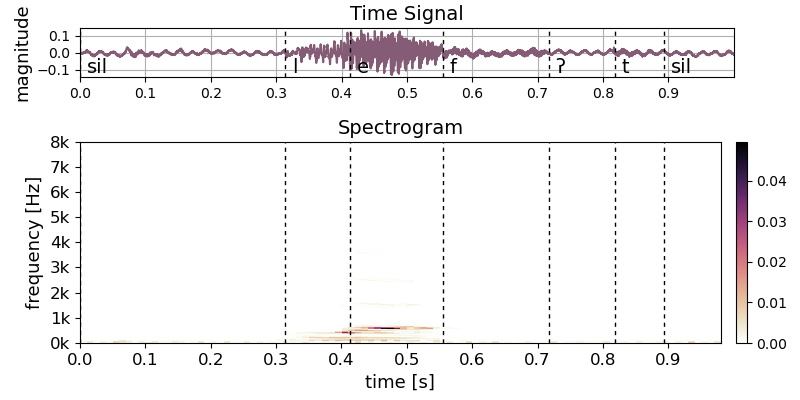
\includegraphics[width=0.45\textwidth]{./3_signal/figs/signal_spec-lin_showcase_left0}}
    \subfigure[right]{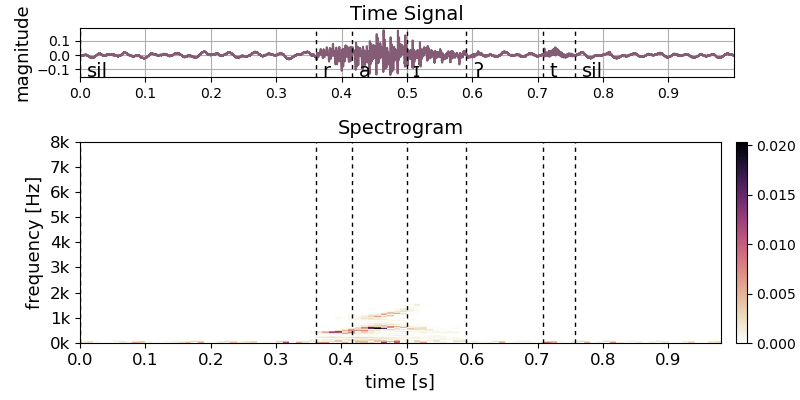
\includegraphics[width=0.45\textwidth]{./3_signal/figs/signal_spec-lin_showcase_right0}}
    \subfigure[up]{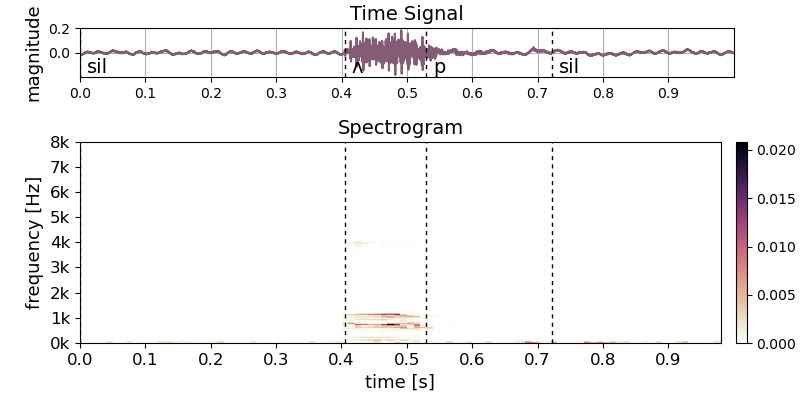
\includegraphics[width=0.45\textwidth]{./3_signal/figs/signal_spec-lin_showcase_up0}}
    \subfigure[down]{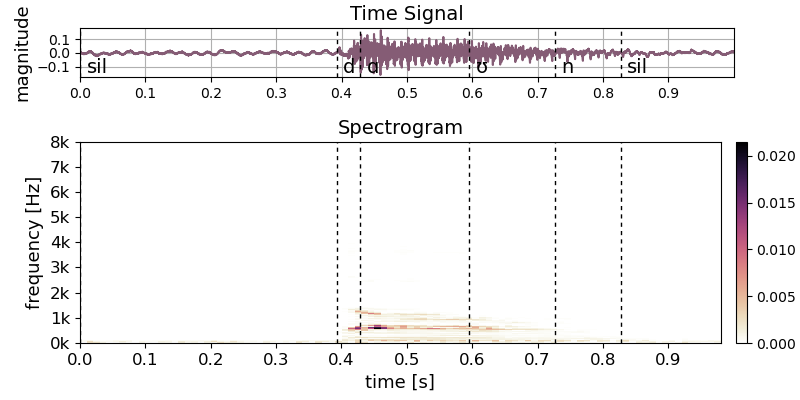
\includegraphics[width=0.45\textwidth]{./3_signal/figs/signal_spec-lin_showcase_down0}}
    \subfigure[go]{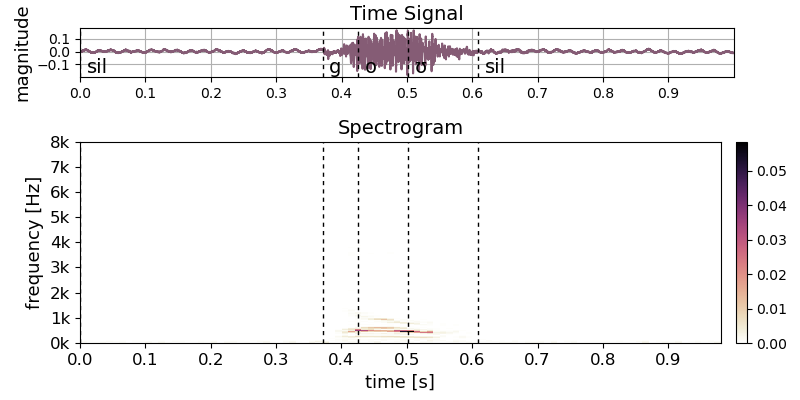
\includegraphics[width=0.45\textwidth]{./3_signal/figs/signal_spec-lin_showcase_go0}}
  \caption{Spectrogram linear scaled.}
  \label{fig:signal_spec_lin_showcase}
\end{figure}
\FloatBarrier
\noindent
It can be observed, that most of the signals energy is in the lower frequency regions of under approximately \SI{1}{\kilo\hertz}, therefore it is more appealing to transform the spectrogram into the log scale of its value space, achieved by:
% --
% log
\begin{equation}\label{eq:signal_spec_log}
  P_{DB} = 10 \cdot \log{P}
\end{equation}
so that small energies are more emphasized with $P_{DB} \in \R^{K \times M}$. 
The same examples with log scaling in the value space visualized with log scaling of the frequency space in the plots are shown in \rfig{signal_spec_log_showcase}.
\begin{figure}[!ht]
  \centering
    \subfigure[left]{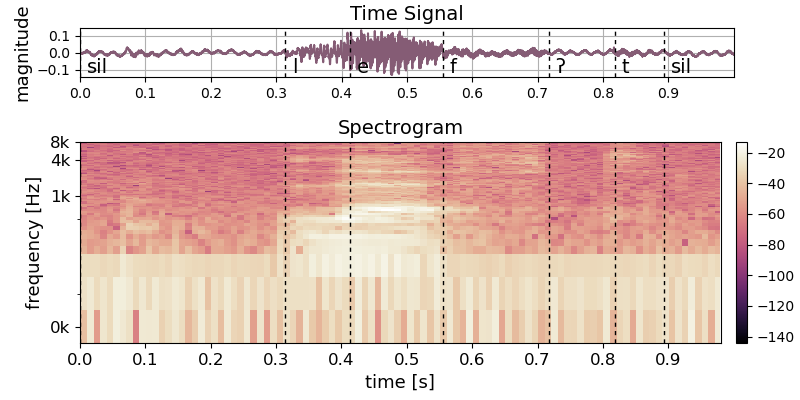
\includegraphics[width=0.45\textwidth]{./3_signal/figs/signal_spec-log_showcase_left0}}
    \subfigure[right]{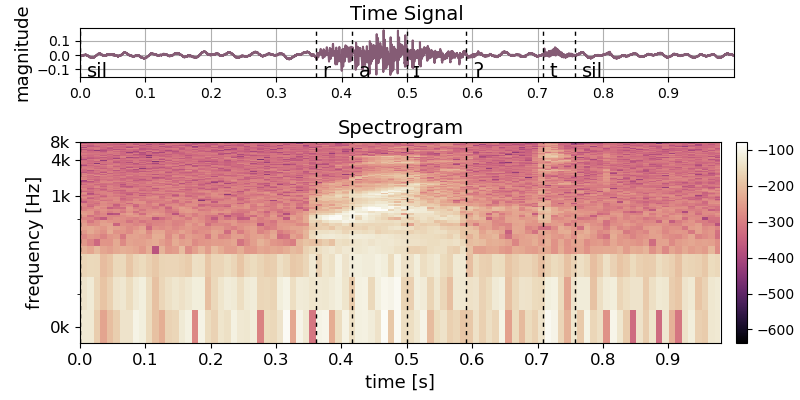
\includegraphics[width=0.45\textwidth]{./3_signal/figs/signal_spec-log_showcase_right0}}
    \subfigure[up]{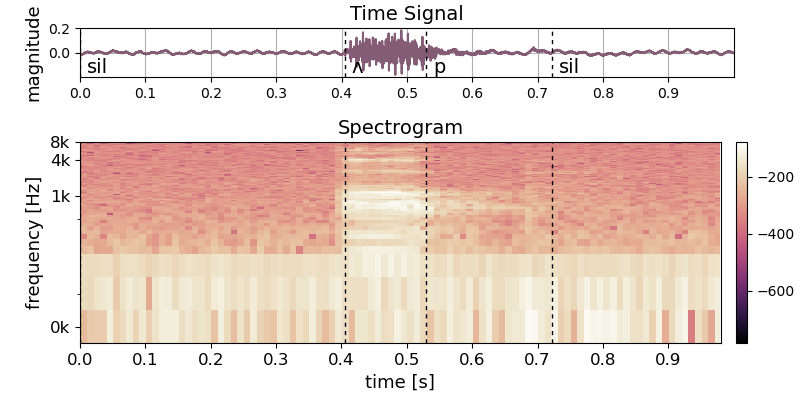
\includegraphics[width=0.45\textwidth]{./3_signal/figs/signal_spec-log_showcase_up0}}
    \subfigure[down]{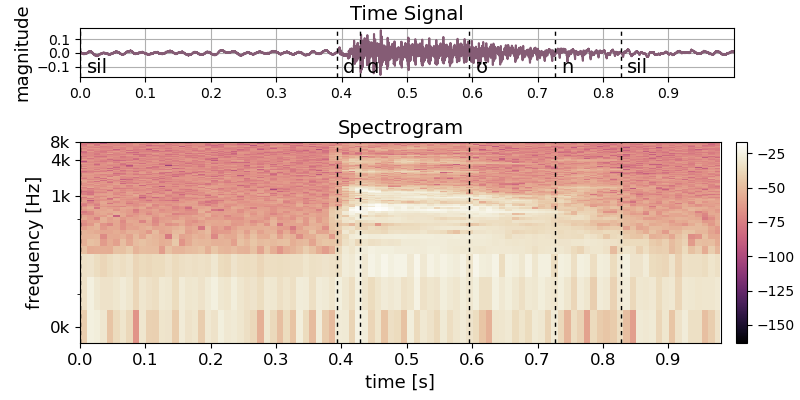
\includegraphics[width=0.45\textwidth]{./3_signal/figs/signal_spec-log_showcase_down0}}
    \subfigure[go]{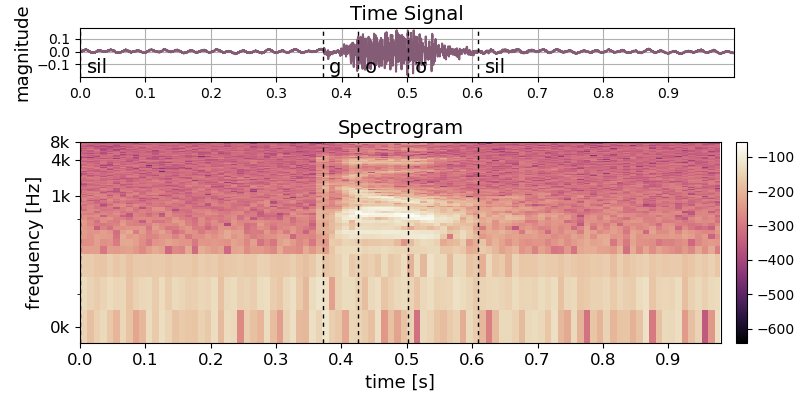
\includegraphics[width=0.45\textwidth]{./3_signal/figs/signal_spec-log_showcase_go0}}
  \caption{Spectrogram logarithmic scaled.}
  \label{fig:signal_spec_log_showcase}
\end{figure}
\FloatBarrier
\noindent
It is now possible to observe some interesting structures and movements in certain frequency bands over time.
A compression scheme, such as the Mel Frequency Cepstral Coefficients (MFCC) explained in the next section, reduces the high dimensional frequency feature vectors of the STFT to more compact feature vectors and further improves the visualization of the spoken command words.
% --
% mfcc

\section{Mel Frequency Cepstral Coefficients}\label{sec:signal_mfcc}
\thesisStateRevised
Very commonly Mel Frequency Cepstral Coefficients (MFCC) are used as input features for neural network classifications tasks in speech recognition.
It is described why MFCCs are good features for speech signals, how they are calculated in detail, how they can be enhanced and in which way they can be visualized to understand them better.


% --
% idea

\subsection{The Idea}
The processing scheme of MFCCs \cite{Mermelstein1980} is as following:
Raw audio samples are transformed into the frequency domain with the Short-Time Fourier Transform (STFT).
Afterwards the power spectrum of the STFT is segmented in frequency bands (along the frequency dimension) done by a filter bank.
The filter bands are spaced in equidistant Mel frequencies, where Mel frequencies represent the non-linear relationship between the Mel and frequency scale.
The Mel scale was developed in psycho-acoustic experiments, where researchers found out, that high frequency sounds (above approximately \SI{500}{\hertz}) are perceived lower than they actual are in the musical sense of pitch.
In the musical sense, a pitch interval of an octave is the doubling of the frequency of a fundamental frequency, but human hearing is different in the perception and frequency doubling does not necessarily double the perceived pitch.
As conclusion the Mel scale is suited human hearing perception of pitch and taking equidistant Mel bands is a reasonable approach.

Another important processing step is the logarithmic scaling of the power spectrum's value space, because humans perceive loudness in the logarithmic scale.
The last step is not that straight forward, but is a technique widely used in image processing called the Discrete Cosine Transform (DCT).
Note that the DCT is some kind of decorrelation process to mix filter bands in different constellations together.

This processing steps seem rather complicated, but are in fact nothing else but consecutive steps of appropriate scaling and data compression.
In fact neural networks are able to handle large amounts of input features, but it is always preferable to minimize the input size, hence the model size and training time are decreased and therefore computations saved.


% --
% processing pipeline

\subsection{Processing Pipeline in detail}\label{sec:signal_mfcc_pipeline}
The frequency spectrum is separated into filter bands through triangular window functions.
Those window functions are equidistantly placed onto the Mel scale and therefore give a varying number of frequency bins in the frequency scale of each window.
The lower frequency bands receive less frequency bins than the high frequency bands.
Sometimes the height of the triangular windows are scaled down so that the effect of unequal amounts frequency bin numbers is equalized, however high frequencies carry less energy and therefore this scaling is in most cases not needed, therefore all the triangular windows have their peak at the value $1$.
The Mel - Frequency relation can be approximated with:
% mel
\begin{equation}\label{eq:signal_mfcc_mel}
  m(f) = 2595 \cdot \log_{10} \left(1 + \frac{f}{700} \right) 
\end{equation}
where $m$ is the result in Mel scale as function of the frequency $f$.
The Mel scale plotted against the frequency scale is illustrated in \rfig{signal_mfcc_mel_scale}.
% mel fig
\begin{figure}[!ht]
  \centering
  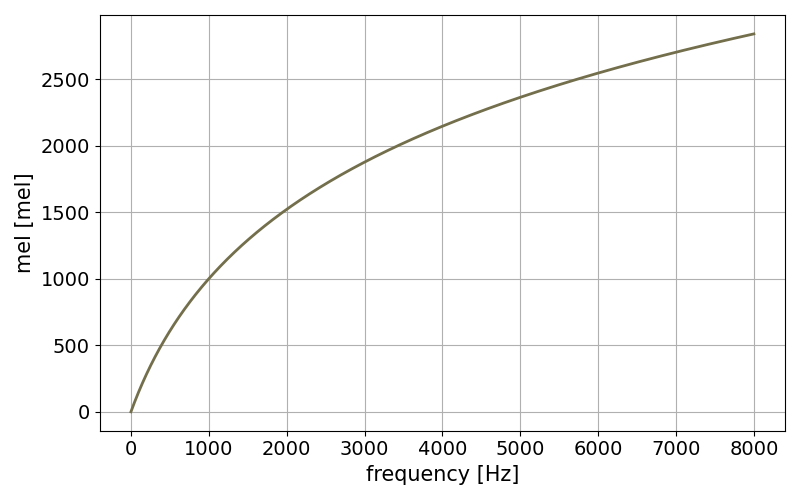
\includegraphics[width=0.40\textwidth]{./3_signal/figs/signal_mfcc_mel_scale}
  \caption{Mel scale as function of the frequency in a range of [0, \SI{16}{\kilo\hertz}].}
  \label{fig:signal_mfcc_mel_scale}
\end{figure}
\FloatBarrier
\noindent
The Mel and frequency window functions or equidistant Mel filter bands are shown in \rfig{filter_bands}.
\begin{figure}[!ht]
  \centering
  \subfigure[mel space]{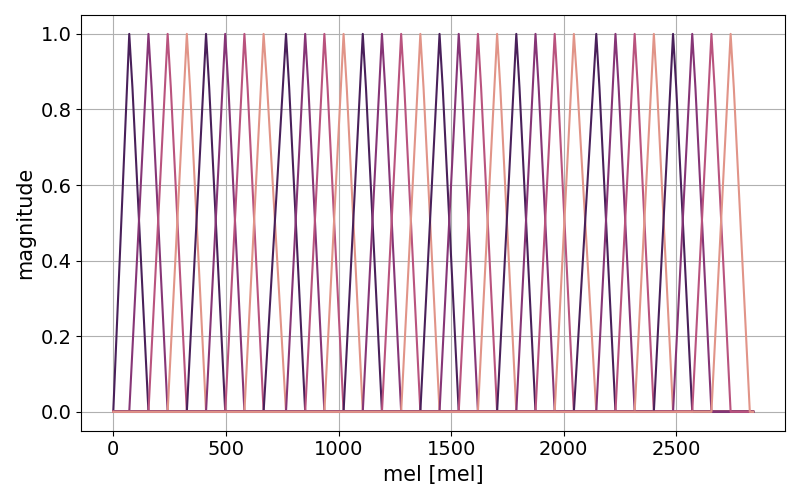
\includegraphics[width=0.40\textwidth]{./3_signal/figs/signal_mfcc_weights_mel}}
  \quad
  \subfigure[frequency space]{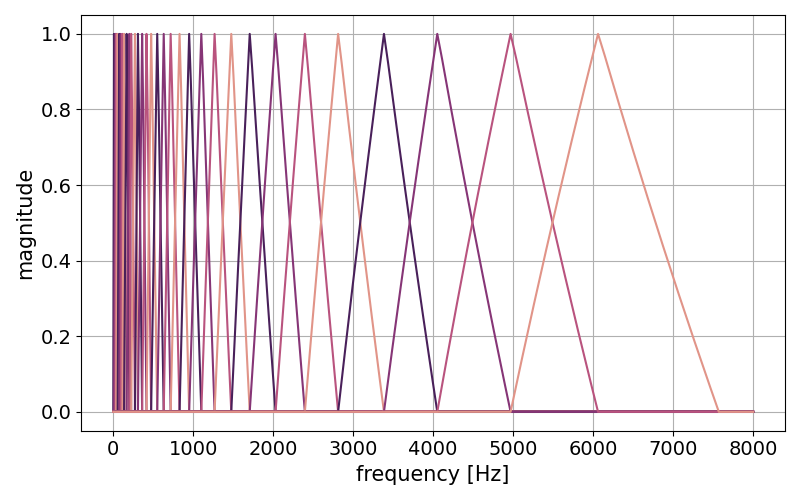
\includegraphics[width=0.40\textwidth]{./3_signal/figs/signal_mfcc_weights_f}}
  \caption{Equidistant Mel filter bands with a total number of 32 bands.}
  \label{fig:filter_bands}
\end{figure}
\FloatBarrier
\noindent
The creation of those filter bands is not described mathematically, because the graphical showcase is much more intuitive and easier to understand.
For further calculations, those filter bands are notated in a weight matrix called $W_m \in \R^{B \times N}$, where $B$ are the amount of used filter bands as rows in the matrix and $N$ the amount of frequency bins of the DFT transformed input signal as columns.

% dct
The DCT is very similar to the Fourier transform and projects the input signal to a set of orthogonal basis functions, however the transformed signal is real valued only instead of complex valued.
Different types of DCTs formulations exists, but most commonly the \enquote{type 2} DCT is used and can be calculated as:
% dct
\begin{equation}\label{eq:signal_mfcc_dct}
  X[c] = \sum_{n=0}^{N-1} x[n] \, \cos{\left[ \frac{\pi}{N} \left( n + \frac{1}{2} \right) c \right]}
\end{equation}
with $c$ as DCT coefficient index and $n$ as sample index of a signal with total length of $N$.
This can be conveniently written in matrix notation with a total number of $C$ DCT coefficients:
% dct matrix
\begin{equation}\label{eq:signal_mfcc_dct_matrix}
  X =  x^T \, \mathcal{D} \quad \mathrm{with} \quad \mathcal{D}[n, c] = \cos{\left[ \frac{\pi}{N} \left( n + \frac{1}{2} \right) c  \right]}, 
  \quad n, c = (0, 1 \dots N - 1), (0, 1 \dots C) 
\end{equation}
with $\mathcal{D} \in \R^{N \times C}$ as DCT matrix and input signal $x \in \R^N$ which gives the transformed signal $X \in \R^C$
The DCT basis functions illustrated in a matrix in two different color schemes are shown in \rfig{signal_mfcc_dct}.
\begin{figure}[!ht]
  \centering
  \subfigure[DCT with continuous color scheme]{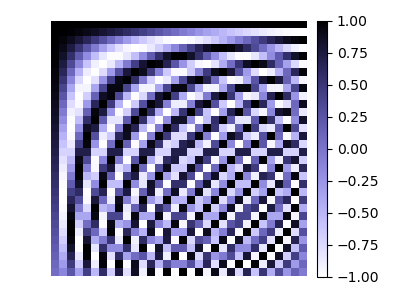
\includegraphics[width=0.35\textwidth]{./3_signal/figs/signal_mfcc_dct}}
  \quad
  \subfigure[DCT with diverging color scheme]{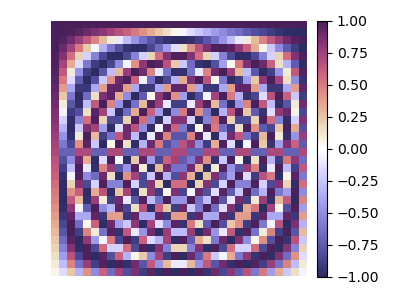
\includegraphics[width=0.35\textwidth]{./3_signal/figs/signal_mfcc_dct-div}}
  \caption{DCT matrix with 32 basis functions illustrated with a continuous and a diverging color scheme.}
  \label{fig:signal_mfcc_dct}
\end{figure}
\FloatBarrier
\noindent
The MFCCs $U \in \R^{M \times C}$ are calculated from the log scaled power spectrum of the STFT $\tilde{X} \in \C^{M \times K}$ computed in \req{signal_spec_stft_matrix}, the filter band weights collected in the matrix $W_m \in \R^{B \times K}$ and transformed with the DCT matrix $\mathcal{D} \in \R^{B \times C}$ as following:
\begin{equation}\label{eq:signal_mfcc_mfcc}
    U = \log{ \left[ \, \abs{\tilde{X}}^2 \, W_m^T \, \right] } \, \mathcal{D}.
\end{equation}
Note that the rows represent all shifts with the hop size and the columns are the individual cepstral coefficients of $U$.
The parameters to choose from are therefore the amount of filter bands $B$ and the amount of cepstral coefficients $C$.

Another important aspect is the visualization of MFCC features.
MFCCs computed as shown above, are not well intended for visualizations, because their individual coefficients value space differs strongly from each other.
For example the first coefficient equals a summation of all filter bands of the spectrogram and is therefore some kind of energy measure, while the other coefficients are different weighted sum combinations of the filter bands.
Further the most of the signal energy is located in the lower frequency bands, which impacts the value space of the coefficients with strongly weighted low frequency bands.
The differences in the value space leads to a problem in the visualization with a linear color scheme, so that some coefficients changes cannot be shown appropriately.
A solution to this problem is to normalize the feature vectors over each frame dimension with the infinity norm as:
% frame based normalization
\begin{equation}\label{eq:signal_mfcc_norm}
  \hat{U}[m, c] = \frac{U[m, c]}{\norm{u_c[m]}_\infty} \quad \forall \, m, c = (1, \dots, M), (1, \dots, C)
\end{equation}
where $m$ is again the frame (time) index, $c$ the individual MFCC coefficient and $u_c[m]$ the individual MFCC coefficient vector over all frames.
This equation gives a value space between $[0, 1]$ for each feature vector $u_c[m]$.

A visualization of MFCC features with 32 filter bands and 32 cepstral coefficients with frame based normalization of each coefficient is shown in \rfig{signal_mfcc_showcase_mfcc32}.
\begin{figure}[!ht]
  \centering
    \subfigure[left]{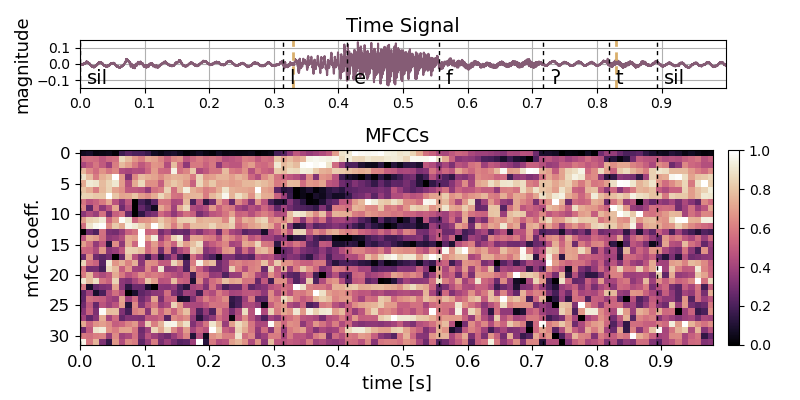
\includegraphics[width=0.45\textwidth]{./3_signal/figs/signal_mfcc_showcase_mfcc32_left0}}
    \subfigure[right]{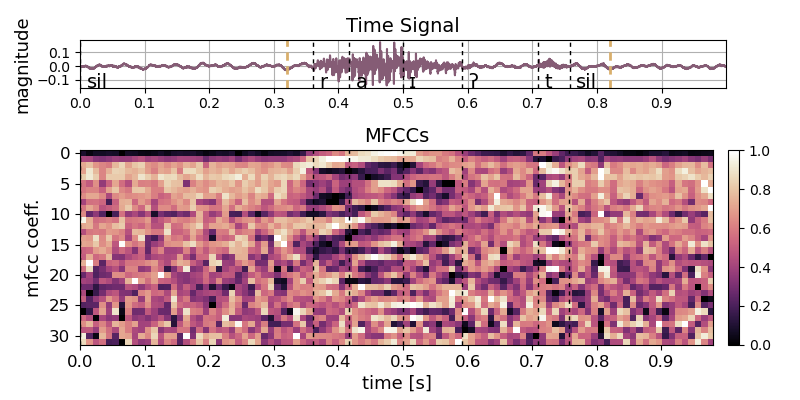
\includegraphics[width=0.45\textwidth]{./3_signal/figs/signal_mfcc_showcase_mfcc32_right0}}
    \subfigure[up]{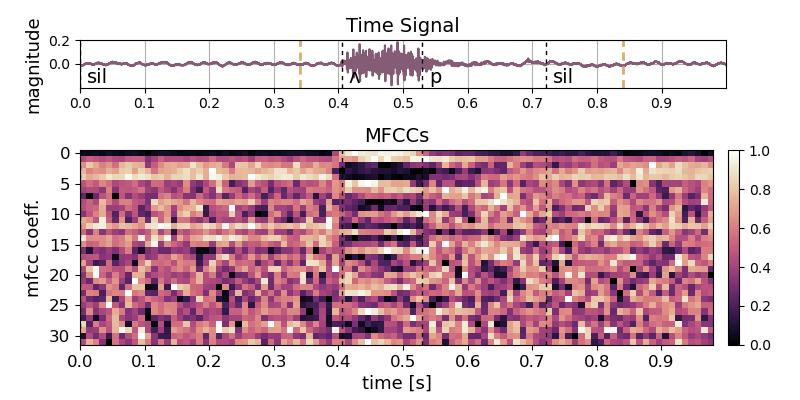
\includegraphics[width=0.45\textwidth]{./3_signal/figs/signal_mfcc_showcase_mfcc32_up0}}
    \subfigure[down]{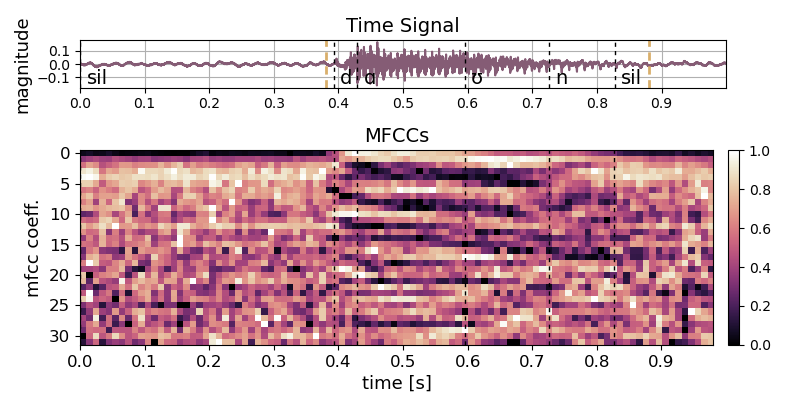
\includegraphics[width=0.45\textwidth]{./3_signal/figs/signal_mfcc_showcase_mfcc32_down0}}
    \subfigure[go]{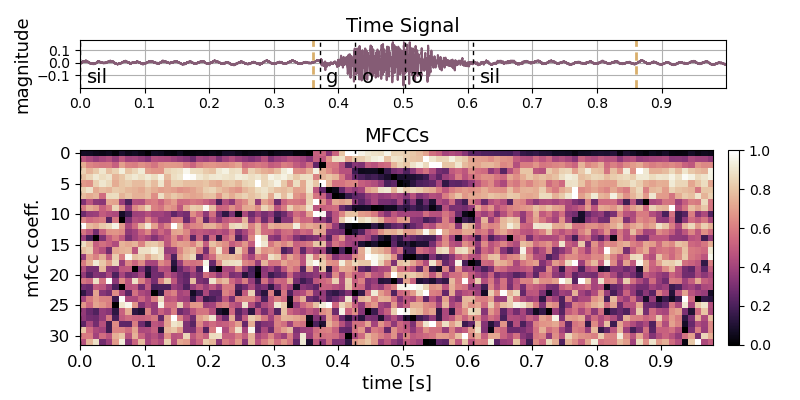
\includegraphics[width=0.45\textwidth]{./3_signal/figs/signal_mfcc_showcase_mfcc32_go0}}
  \caption{MFCC with 32 filter bands and 32 cepstral coefficients visualized with frame-based normalization.}
  \label{fig:signal_mfcc_showcase_mfcc32}
\end{figure}
\FloatBarrier
\noindent
The frame based normalization is an interesting aspect to improve the visualization of the MFCC features, however it can be critical. 
A normalization that operates only in one dimension changes important structures within the feature space and it cannot be answered yet if this is a problem for neural networks or degrades the classification performance.
One more research question arises here: Is it possible to use frame based normalized MFCC features as inputs to neural networks and what are the results to the accuracy and training of the models.


% --
% enhancement

\subsection{MFCC Feature Usage and Enhancement}\label{sec:signal_mfcc_enhancement}
After the MFCCs are computed with the choice of filter bands $B$ and cepstral coefficients $C$, they can already be used as input features for neural networks.
The question arises, whether feature enhancement can improve the performance in classification.
The best practice, applied in many papers, is to use $B=32$, $C=12$, compute derivatives of those 12 MFCC coefficients named as deltas (first derivative regarding the frame dimension) and double deltas (second derivative) and add energy vectors of the 12 coefficients and each one of the deltas.
The deltas are simply computed as frame $m$ difference of the MFCCs with:
\begin{equation}\label{eq:signal_mfcc_delta}
  \Delta u_i[m] = \frac{u_i[m - 1] + u_i[m + 1]}{2}
\end{equation}
where $u_i \in \R^M$ is the i-th MFCC coefficient vector and $m$ the frame index.
Note that the computation of the deltas at the edges $m=0$ and $m=M$ is not possible and the same value is obtained from the neighbor at this specific locations.
The second derivative of MFCC features, known as double deltas, are the frame differences of the deltas and in the same way computed as in \req{signal_mfcc_delta}.
Another enhancement is the computation of an energy feature vector of the MFCCs with:
\begin{equation}
  e[m] = u[m]^T \, u[m] 
\end{equation}
where $u[m] \in \R^C$ is the MFCC feature vector of frame $m$.
The same energy computation may also be applied to the deltas and double deltas each.
The MFCCs, their deltas, double deltas and energy vectors can simply be stacked at top of each other and used as enhanced feature inputs to neural networks.
In this thesis the feature vectors are stacked as following:
\begin{enumerate}
    \item 12 MFCCs
    \item 1 Energy feature of the 12 MFCCs
    \item 12 Deltas
    \item 1 Energy feature of the 12 Deltas
    \item 12 Double Deltas
    \item 1 Energy feature of the 12 Double Deltas
\end{enumerate}
which sums up to a 39-dimensional feature vector, very commonly used in the literature.
Many papers do not explicitly explain how the 39 MFCCs are calculated in detail, in most cases however this constellation is applied.
The computation of 39 MFCCs are shown in \rfig{signal_mfcc_showcase_mfcc39}
\begin{figure}[!ht]
  \centering
    \subfigure[left]{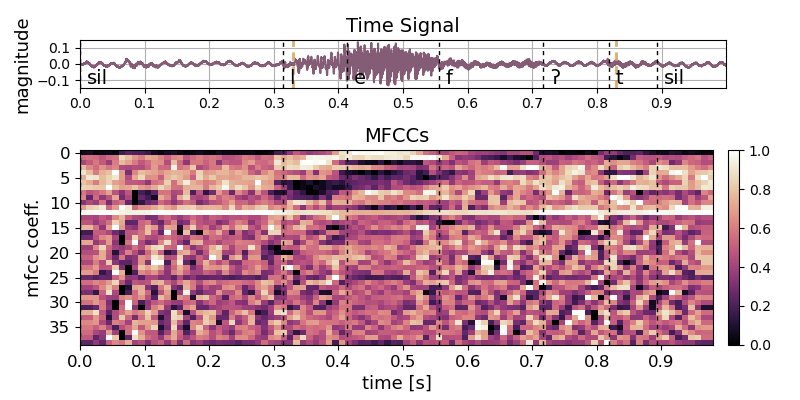
\includegraphics[width=0.45\textwidth]{./3_signal/figs/signal_mfcc_showcase_mfcc39_left0}}
    \subfigure[right]{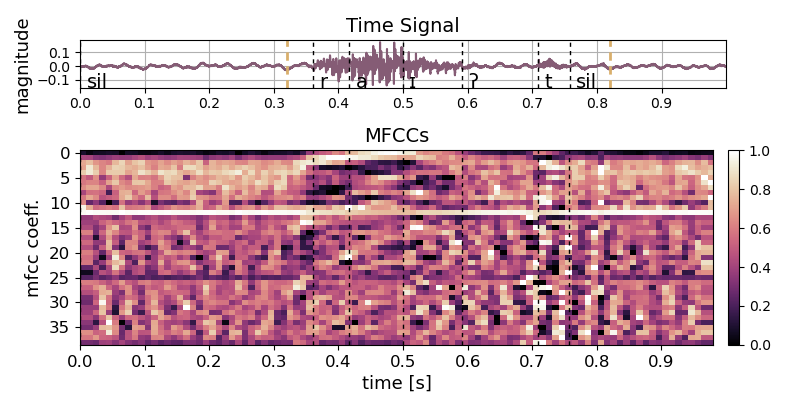
\includegraphics[width=0.45\textwidth]{./3_signal/figs/signal_mfcc_showcase_mfcc39_right0}}
    \subfigure[up]{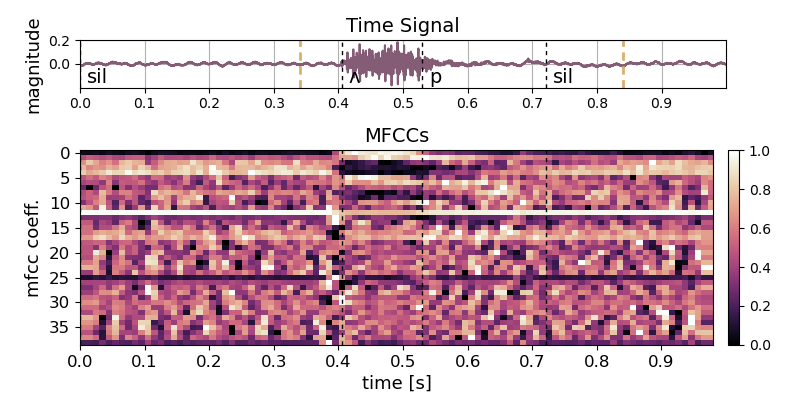
\includegraphics[width=0.45\textwidth]{./3_signal/figs/signal_mfcc_showcase_mfcc39_up0}}
    \subfigure[down]{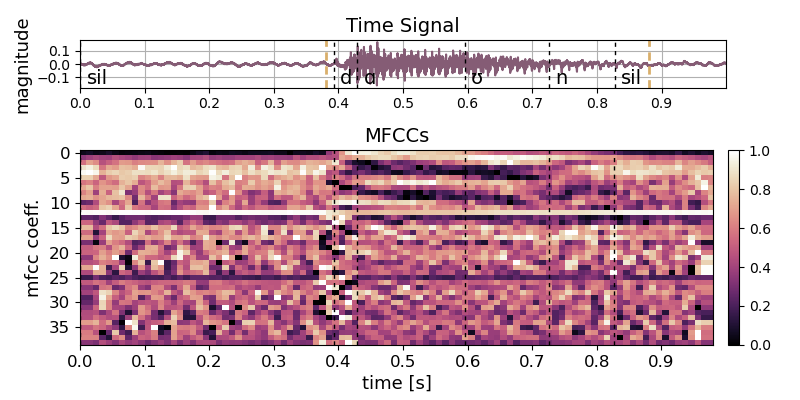
\includegraphics[width=0.45\textwidth]{./3_signal/figs/signal_mfcc_showcase_mfcc39_down0}}
    \subfigure[go]{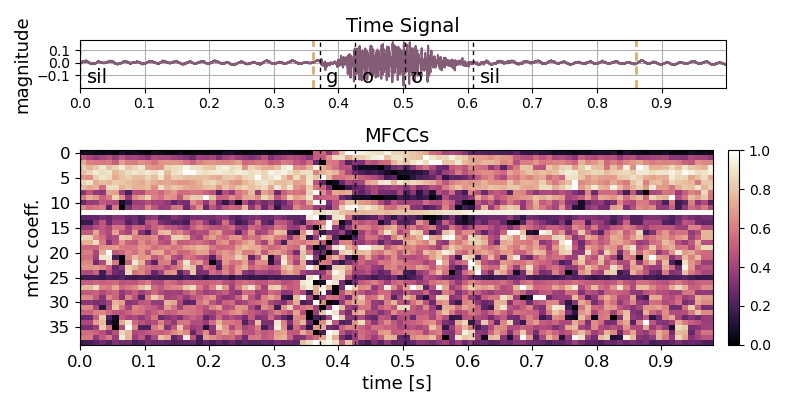
\includegraphics[width=0.45\textwidth]{./3_signal/figs/signal_mfcc_showcase_mfcc39_go0}}
  \caption{MFCC with 32 filter bands and 12 cepstral coefficients, deltas, double deltas and energy vector visualized with frame-based normalization.}
  \label{fig:signal_mfcc_showcase_mfcc39}
\end{figure}
\FloatBarrier
\noindent


% --
% energy consumption

\subsection{Computational Complexity}
The computational complexity is evaluated on the total amount of operations needed for a specific computation task, such as the feature extraction task of MFCCs.
The energy consumption is related to the computational complexity, but it is much harder to define and depends on many small parameters and actual hardware implementations, which is especially important for handheld devices.
The count of operations is sufficient for this thesis and provides a comparison to the benchmark models mentioned in \rsec{prev_kws_benchmark}.
The computational complexity for the computation of MFCC features are the amount of operations needed to process a \SI{1}{\second} time signal sampled with $f_s = \SI{16}{\kilo\hertz}$.
All MFCC specific extraction details are collected in \rtab{signal_mfcc_extraction_params}.
\begin{table}[ht!]
\small
\begin{center}
\caption{Parameters for determining the computational complexity of the MFCC feature extraction process.}
\begin{tabular}{ M{7cm}  M{2.5cm} M{2.5cm}}
\toprule
\textbf{Parameter} & \textbf{Value} & \textbf{Sample Length} \\
\midrule
Length of a signal $n$ & \SI{1}{\second} & 16000 \\
Analytic window size $N$ & \SI{25}{\milli\second} & 400 \\
Hop size $h$ & \SI{10}{\milli\second} & 160\\
\midrule
Fourier coefficients $K$ & 400  & - \\
Number of filter bands $B$ & 32 & -\\
Number of cepstral coefficients $C$ & 12 & -\\
\bottomrule
\label{tab:signal_mfcc_extraction_params}
\end{tabular}
\end{center}
\vspace{-4mm}
\end{table}
\FloatBarrier
\noindent
The amount of operations are the total number of additions and multiplications necessary to fulfill the process.
The major components of the MFCC are, as described in \rsec{signal_mfcc_pipeline} and summarized in \req{signal_mfcc_mfcc}, the transformation to the STFT, the weighting with the filter bands and the DCT transform.
The most costly component is of course the STFT, which again is composed of DFTs.
Note that the DFT uses complex multiplications and additions.
One complex multiplication equals to 4 real multiplication and 2 additions, so one complex multiplication consists of 6 operations.
For one complex addition, two real additions are necessary and equals therefore to 2 operations.
A general matrix multiplication with a vector $y = Ax$ where $A \in \R^{m \times n}$ and $x \in \R^n$ is composed of $m \cdot n$ multiplications and $m \cdot (n - 1)$ additions, where for simplicity the amount of additions is also assumed to be $m \cdot n$.

The amount of operations, denoted as $\mathcal{T(.)}$, for a trivial DFT transform with operator $\mathcal{F} \in \C^{N \times K}$ with $K$ Fourier coefficients on a windowed signal $x \in \R^N$ with sample length $N$ is:
% \begin{equation}
%   \mathcal{O}(x\mathcal{F}) = N \times K
% \end{equation}
\begin{equation}
  \mathcal{T}(x^T \mathcal{F}) = 6 (N K) + 2 (N K)
\end{equation}
and give for $N = K = 400$ the amount of operations $\mathcal{T}(x\mathcal{F}) = \SI{1.28}{\mega\ops}$ for a single DFT.
This of course are a lot of operations, luckily a more sophisticated Fourier transform can be applied with the Fast Fourier Transform (FFT) method, which gives a linear complexity and operations are calculated as:
\begin{equation}
  \mathcal{T}(x^T \mathcal{F}) = 6 (\mathcal{O}(N \cdot \log N)) + 2 (\mathcal{O}(N \cdot \log N))
\end{equation}
with $N = K = 400$.
The FFT has therefore roughly $\mathcal{T}(x^T \mathcal{F}) = \SI{20}{\kilo\ops}$ and is a huge improvement to the trivial method.
Further the interesting part of a DFT or FFT is only the half-band, because of the mirroring effect, which likewise may decrease the operations by half, so let the calculations be continued with Fourier coefficients of $K = 201$ of a half band and roughly $\SI{10}{\kilo\ops}$ per FFT.
The DFT is computed $M$ times, where $M$ is the total number of possible shifts calculated in \req{signal_spec_hop}, which gives with the evaluated parameters $M = 98$ frames.
So for the whole STFT $M$ is multiplied with the number of operations of each DFT, which give approximately $\mathcal{T}(\tilde{X}) = \SI{1}{\mega\ops}$.

The computation to the power spectrum and the log scaling are disregarded, so that two matrix multiplications remain:
$\abs{\tilde{X}}^2 \, W_m^T$ is a matrix multiplication of $\R^{M \times K}$ and $\R^{K \times B}$ which has $M K B$ real multiplications and approximately $M K B$ real additions, which give about $2 M K B = 2 \cdot 98 \cdot 201 \cdot 32 =  \SI{1.26}{\mega\ops}$.
The resulting band weighted STFT matrix $\R^{M \times B}$ is further multiplied with the DCT operator representing a matrix of $\R^{B \times C}$, that gives $2 M B C = 2 \cdot 98 \cdot 32 \cdot 12 = \SI{75}{\kilo\ops}$.
Altogether the matrix multiplications are approximately $\SI{1.26}{\mega\ops} + \SI{75}{\kilo\ops} = \SI{1.34}{\mega\ops}$.

The summary of the estimated operations are listed in \rtab{signal_mfcc_operations}.
% --
% mfcc operations
\begin{table}[ht!]
\begin{center}
\caption{Approximated number operations needed to transform a \SI{1}{s} time signal to MFCCs with parameters listed in \rtab{signal_mfcc_extraction_params}.}
\begin{tabular}{ M{6cm}  M{4cm}}
\toprule
\textbf{Process} & \textbf{Approximated Number of Operations} \\
\midrule
Power spectrum & \SI{2.71}{\mega\ops}\\
Weighting with equidistant Mel bands & \SI{1.26}{\mega\ops}\\
DCT transform of the weighted power spectrum & \SI{75}{\kilo\ops}\\
\midrule
\textbf{Sum} & \SI{4.05}{\mega\ops}\\
\bottomrule
\label{tab:signal_mfcc_operations}
\end{tabular}
\end{center}
\vspace{-4mm}
\end{table}
\FloatBarrier
\noindent


% --
% critism

\subsection{Criticism}
\thesisStateNew
MFCC are widely used for speech recognition tasks and perform very well, however the processing pipeline of MFCC has some disadvantages.
One disadvantage is, as already mentioned, that MFCCs are not intended for visualization, because of their broad value space of individual MFCC coefficients.
Another disadvantage is, that MFCC are not directly invertible to raw audio samples, because of the computation of the spectrogram.
Some inversion techniques exist \cite{Boucheron2008}, but it is still a rough approximation.
The inversion of MFCC would have been very interesting, when applied to generative neural networks, such as Generative Adversarial Neural Networks (GAN).



% --
% visualization

%\subsection{Visualization of MFCC features}\label{sec:signal_mfcc_visualization}


%To show this difference in value space in a negative example in practice, the MFCCs of the self-recorded speech command waveform \enquote{left0.wav} is shown in \rfig{left0_mfcc_only}.
% useless
% \begin{figure}[!ht]
%   \centering
%     \includegraphics[width=0.75\textwidth]{./3_signal/figs/signal_mfcc_left0_mfcc_only.png}
%   \caption{Bad visualisation of the 12 MFCCs features extracted from \enquote{left0.wav}.}
%   \label{fig:left0_mfcc_only}
% \end{figure}
% \FloatBarrier
% \noindent
% Not much structure of the MFCCs can be seen here, due to the vast value difference of the first coefficient. At least the first coefficient shows, where the center of signal energy is placed on the time scale, but other than that, this visualisation is worthless.
% Another very bad visualisation is shown by computing the 39 MFCC feature vectors (with Deltas, Double Deltas and Energies) in \rfig{left0_no_order}.

% \begin{figure}[!ht]
%   \centering
%     \includegraphics[width=0.75\textwidth]{./3_signal/figs/signal_mfcc_left0_no_order_norm0.png}
%   \caption{Very bad visualisation of 39 MFCC features extracted from \enquote{left0.wav}.}
%   \label{fig:left0_no_order}
% \end{figure}
% \FloatBarrier
% \noindent
% There appears an even greater gap of different value spaces and even less is seen.

% One solution is to show the features in different value groups. 
% For instance putting the first coefficient and its deltas is in one group, the other coefficients in another and their deltas and energies as well in own groups. 
% Now it is possible to observe some structure in the visualizations, with an example shown in \rfig{left0_order}.

% \begin{figure}[!ht]
%   \centering
%     \includegraphics[width=0.75\textwidth]{./3_signal/figs/signal_mfcc_left0_norm0.png}
%   \caption{Good visualisation of 39 MFCC features extracted from \enquote{left0.wav} with own value groupings.}
%   \label{fig:left0_order}
% \end{figure}
% \FloatBarrier
% \noindent
% Another way to improve the visualization is to normalize the feature vectors over each frame dimension with the infinity norm as:

% % frame normalisation
% \begin{equation}\label{eq:signal_mfcc_norm}
%   \hat{U}[m, l] = \frac{U[m, l]}{\norm{u_l[m]}_\infty}
% \end{equation}
% where $m$ is again the variable in frames, $l$ the individual MFCC coefficient and $u_l[m]$ the individual MFCC coefficient vector over all frames.
% This equation gives a value space between $[0, 1]$ for each feature vector $u_l[m]$.

% A visualization with frame normalization of the 39 MFCC feature vectors of \enquote{left0.wav} is shown in \rfig{left0_order},

% \begin{figure}[!ht]
%   \centering
%     \includegraphics[width=0.75\textwidth]{./3_signal/figs/signal_mfcc_left0_no_order_norm1.png}
%   \caption{Normalization of 39 MFCC features extracted from \enquote{left0.wav}.}
%   \label{fig:left0_no_order_norm1}
% \end{figure}
% \FloatBarrier
% \noindent
% or in an even better one shown in \rfig{left0_order_norm1}.

% \begin{figure}[!ht]
%   \centering
%     \includegraphics[width=0.75\textwidth]{./3_signal/figs/signal_mfcc_left0_order_norm1.png}
%   \caption{Normalisation of 39 MFCC features extracted from \enquote{left0.wav} with groups.}
%   \label{fig:left0_order_norm1}
% \end{figure}
% \FloatBarrier
% \noindent

% --
% onset

\section{Onset Detection}\label{sec:signal_onset}
\thesisStateReady
\thesisStateNew
Onset detection of key words is an essential part in Key Word Spotting (KWS) systems and describes the starting time of an actual key word.
In this thesis the onset detection is separated into:
\begin{itemize}
  \item key word onset detection (within a fixed time span)
  \item online onset detection
\end{itemize}
the key word onset detection is performed on already extracted time signals, such as raw data examples from the dataset, where the time interval of those signals are limited to \SI{1}{\second}.
The online onset detection runs during the recording of potential key words from a microphone input in a real time system.
Note that onset detection can be quite challenging and is of some sorts an own research subject.
For this thesis, however it is enough to use trivial methods, that do not use much computational effort.


% --
% key word onset detection

\subsection{Key Word Onset Detection}\label{sec:signal_onset_kw}
An intuitive method to detect the onsets of key words in a fixed time signal, is to simply use the signal energy.
Consider a fixed time signal $\bm{x} \in \R^n$ with a total number of $n$ samples, that is windowed with a striding frame of sample length $N$ corresponding to a time duration of \SI{500}{\milli\second}, the energy of each windowed signal is calculated as:
\begin{equation}\label{eq:e_win}
  e[m] = \sum_{i=0}^{N-1} \abs{x[m + i]}^2
\end{equation}
with shift index $m \in \mathcal{M} = \{0, 1, \dots, n - N + 1\}$.
The onset sample number $o \in \mathcal{M}$ with the highest energy region can be determined by
\begin{equation}\label{eq:onset}
  o = \underset{m \in \mathcal{M}}{\arg \max} \, e[m]
\end{equation}
for all windowed signal energies $e[m]$.
Note that it is assumed, that most of the key word in each signal is captured by the window length $N$ and that no noise peaks are present before and after the key word, otherwise the onset $o$ is shifted to either the left or right-hand side of the actual key word onset.
It is for sure, that this onset detection is not the most reliable one, but it is the simplest and most energy efficient method performed on raw audio data.

A better approach is to use energy values from the frequency response of the signal.
Since the Mel Frequency Cepstral Coefficients (MFCC) are extracted to obtain features for neural networks, it is straight forward to use them for onset detection as well.
The first cepstral coefficient $\bm{u}_0 \in \R^M$ of the MFCCs is actually an energy value, that is the sum of all equidistant mel filter bands.
The equivalent of \req{e_win} for MFCCs in the cepstral and frame space is therefore:
\begin{equation}
  e[m] = \sum_{i=0}^{N-1} \bm{u}_0[m + i]
\end{equation}
where $m$ and $N$ are in the frame space instead of the sample space.
A conversion from sample to frame space can simply be done by dividing the sample variable with the hop size $h$ in samples and rounding it to an integer number.
The onset frame $o$, using the first MFCC coefficient, is determined in the same way as formulated in \req{onset}.
An illustration of the onset detection with the fixed window of size \SI{500}{\milli\second} is shown in \rfig{signal_onset_window}, where
the start of the striding window with the highest energy value contained in this window, is the onset.
\begin{figure}[!ht]
  \centering
    
\includegraphics[width=0.55\textwidth]{./3_signal/figs/signal_onset_window}
  \caption{Striding window length of \SI{500}{\milli\second} used for energy calculation in onset detection.}
  \label{fig:signal_onset_window}
\end{figure}
\FloatBarrier
\noindent
A showcase on the performance of both energy onset detection methods are shown in \rfig{signal_onset_showcase}.
\begin{figure}[!ht]
  \centering
    \subfigure[left]{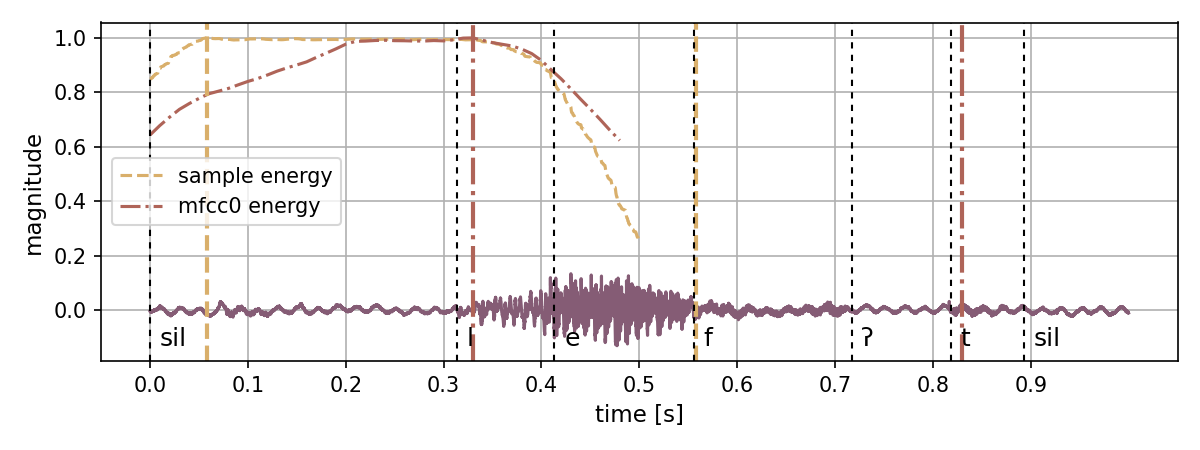
\includegraphics[width=0.45\textwidth]{./3_signal/figs/signal_onset_showcase_left0}}
    \subfigure[right]{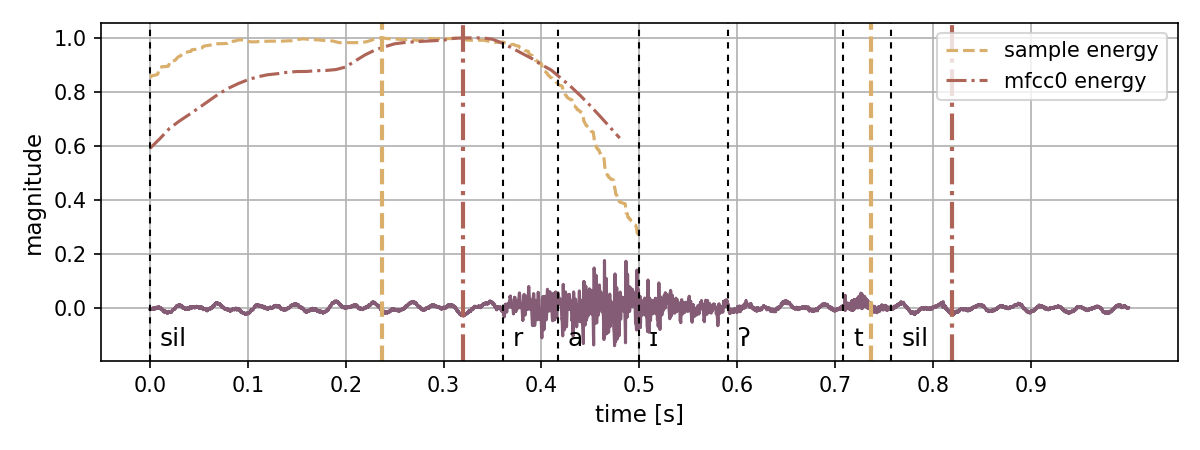
\includegraphics[width=0.45\textwidth]{./3_signal/figs/signal_onset_showcase_right0}}
    \subfigure[up]{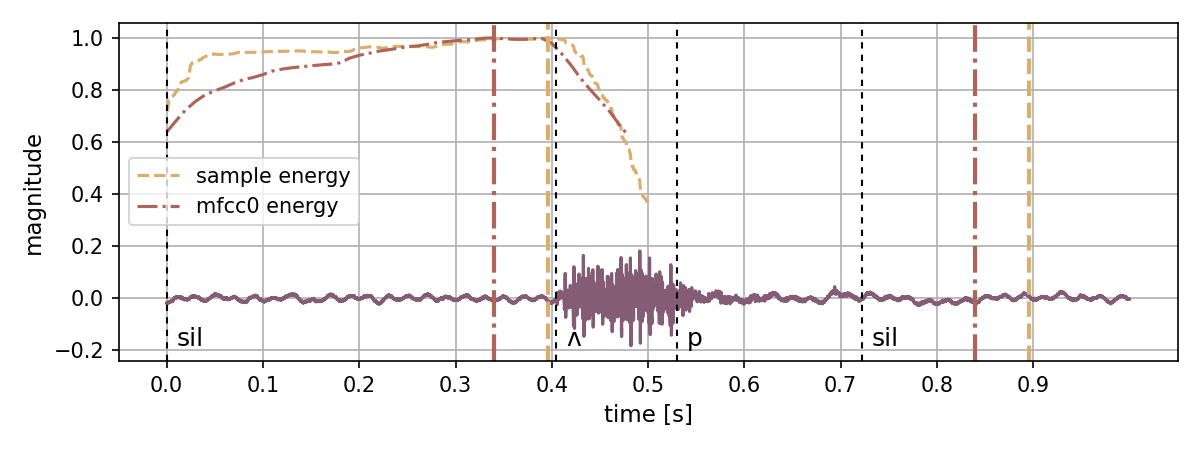
\includegraphics[width=0.45\textwidth]{./3_signal/figs/signal_onset_showcase_up0}}
    \subfigure[down]{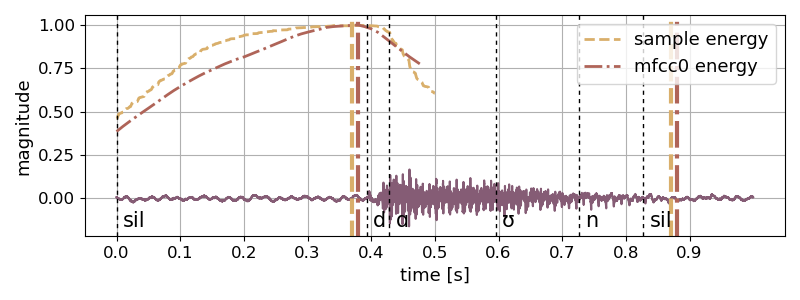
\includegraphics[width=0.45\textwidth]{./3_signal/figs/signal_onset_showcase_down0}}
    \subfigure[go]{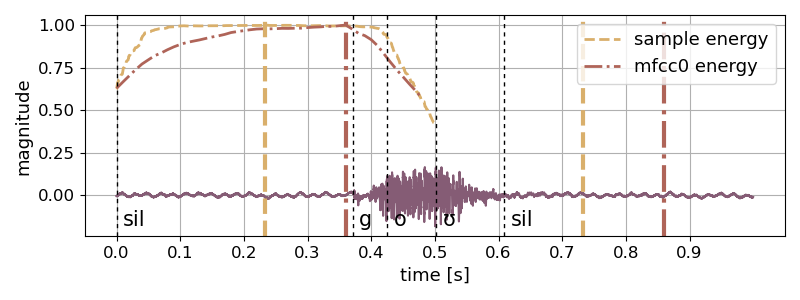
\includegraphics[width=0.45\textwidth]{./3_signal/figs/signal_onset_showcase_go0}}
  \caption{Onsets (vertical colored lines) obtained from the maximum of either the sample energy or first MFCC coefficient energy, with an analytical window length of \SI{500}{\milli\second}.}
  \label{fig:signal_onset_showcase}
\end{figure}
\FloatBarrier
\noindent
It can be observed that the MFCC onset method works much better, especially for the \enquote{left} example, where a little noise peak shifts the sample energy onset too far to the left so that the whole word is not captured.
For all MFCC extractions from the datasets during the experiments, the MFCC onset method is used. 
For raw audio extraction, applied in Wavenets, the sample energy method is applied.


% --
% key word onset detection

\subsection{Online Onset Detection}\label{sec:signal_onset_online}
The onset detection of online speech signals received from a microphone input stream, is processed by evaluating consecutive input chunks, that are stored in an input buffer.
From those input chunks the energy level can be computed and compared with an energy threshold, that should indicate the presence of an onset.
It is not the purpose to detect key word onsets by its correct starting time, but to signalize that a signal with enough energy is available for a potential key word classification.
Mathematically the onset $o(\bm{x}) \in \{0, 1\}$ of an input chunk $\bm{x} \in \R^n$ from an actual microphone input stream, can be obtained by:
\begin{equation}
  o(\bm{x}) = 
  \begin{cases}
    1, & \text{if } \frac{1}{n} \bm{x}^T \bm{x} > \alpha\\
    0, & \text{otherwise} 
  \end{cases}
\end{equation}
where the output value of $1$ represents the occurance of an onset, $n$ is the total sample number of the input chunk and $\alpha$ the energy threshold.
The energy threshold should be adjustable to the users microphone and ampliefier setup. 
This can be done for instance in the video game option menu as described in \rsec{game_interactables_menu}.
If an online onset is detected, the whole buffer is filled up first, then read and MFCC features extracted.
From those MFCCs the exact key word onset is calculated as described in \rsec{signal_onset_kw} and the \SI{500}{\milli\second} long feature vectors are sent to the classification system.

% --
% Neural Network

\chapter{Neural Networks}\label{sec:nn}
This chapter contains theoretical foundations to understand the structure of the used neural networks architectures applied to the Key Word Spotting (KWS) task of speech commands.
Each used neural network architecture is described in detail.
Special focus is lied on energy efficiency and therefore each networks energy footprint is evaluated.
Strategies for adversarial training are shown.

% theory
% --
% theory

\section{Theory}\label{sec:nn_theory}
\thesisStateNotReady
The theory provided in this sections merely focuses on the used neural network architectures and some basic theory elements in neural networks.
The most basic element in neural networks is described here as node, an abstract element, usually illustrated as circle, that defines input and output connections from and to other nodes within the network.
The connections from and to a node are multiplications with scalar values, denoted as weight.
Each node usually incorporates an additive term, denoted as bias term.
All weights and bias terms are forming the parameters of a network and can be trained through back-propagation.
The output of a node is a scalar computed from all inputs and mapped with a non-linear function denoted as activation function.
A neural network can consist of thousand of nodes in each possible constellation of connections.
In this thesis, the focus is only on single directional connections (no bidirectional connections).
The structure of a neural network is defined by its layers, where a layer is a set of nodes with specific connection properties that receive inputs from the previous layer and output connections to the next layer.
For example, a neural network consists one convolutional layer followed by three fully connected layers.
The last layer of a neural network represents for instance the class labels of a classification tasks.
A loss function computes the difference between the predicted and the actual class label during training and is essential for the backpropagation algorithm that updates each parameter in the network through the gradients of the obtained error.


% --
% activation functions

\subsection{Activation Functions}\label{sec:nn_theory_acti}
Activation functions for neural networks of a node in a current layer are non-linear functions that usually maps the sum of the weighted inputs from nodes in a previous layer to a single output value $z$ as following:
\begin{equation}\label{eq:nn_theory_acti}
  z = h(w \, x^T)
\end{equation}
where $h$ is the activation function, $w \in \R^n$ is an weight vector and $x \in \R^n$ an input vector for one specific node.
The output of each node in a current layer is further connected to other nodes in the next layer and builds up the neural network.
The constraint of an activation function is, that an easy computable derivative of this function exist, in order to backpropagate gradients.

The most famous activation function nowadays is the RELU function:
\begin{equation}\label{eq:nn_theory_relu}
  z = \max{(0, a)}
\end{equation}
with $a \in \R$ as input to the activation function.
The big advantage is that this function and its subgradients are very easy and fast to compute.
The two other activation functions that are used in wavenets are the sigmoid function:
\begin{equation}\label{eq:nn_theory_sigmoid}
  z = \frac{1}{1 + \exp{-x}}
\end{equation}
and the tanh functions:
\begin{equation}\label{eq:nn_theory_tanh}
  z = \frac{\exp{x} - \exp{-x}}{\exp{x} + \exp{-x}}
\end{equation}


% --
% fully connected

\subsection{Fully Connected Layer}
A fully connected (FC) layer is the simplest layer type in neural networks.
Each node from the previous layer is connected in forward direction to all nodes in the FC layer and each node in the FC layer is further connected to all nodes in the next layer.
Further each connection has one trainable weight and each node has a bias term.
A simple FC layer is illustrated in \rfig{nn_theory_fc}.
% fc
\begin{figure}[!ht]
  \centering
    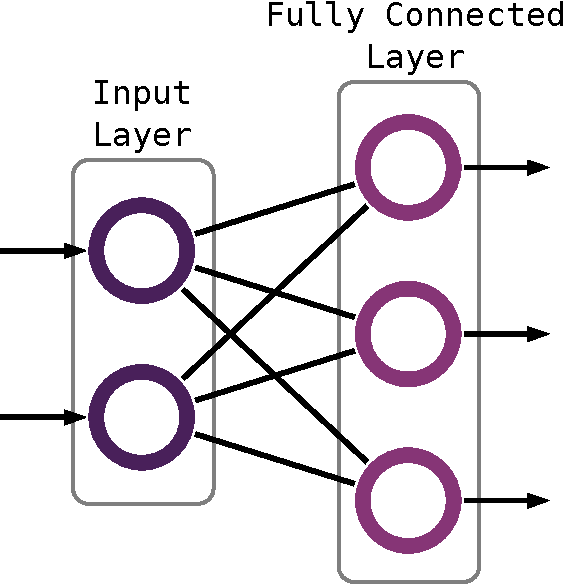
\includegraphics[width=0.30\textwidth]{./4_nn/figs/nn_theory_fc.eps}
  \caption{Basic fully connected layer with 3 nodes, receiving connections from 2 input nodes and outputing connections to 2 output nodes.}
  \label{fig:nn_theory_fc}
\end{figure}
\FloatBarrier
\noindent
In one node usually following computation is processed:
\begin{equation}
  z = h(w \, x^T + b)
\end{equation}
with the same notations as in \req{nn_theory_acti} and an additional bias term $b \in \R$.


% --
% cnn

\subsection{Convolutional Layers}\label{sec:nn_theory_cnn}
Convolutional layers are the fundament of every Covolutional Neural Networks (CNN) as already discussed in \rsec{prev_nn_cnn}.
They use convolutional filters on small areas of the input data, so that spatial information is retrieved.
Those convolutional filters are also called kernels and illustrated in case of images as rectangle in 2D space with kernel width $k_w$ and height $k_h$.
The kernel is shifted over its input map in each axis with an operation called \emph{stride}, denoted as $s$, and produce a output map through convolution.
The output dimension $o_d$ for striding along this axis with $s_d$ and kernel size for that axis $k_d$ over the input dimension $i_d$ can be computed as:
\begin{equation}\label{eq:nn_theory_cnn_}
  o_d = \floor*{\frac{i_d + p_d - k_d}{s_d} + 1}
\end{equation}
where $p_d$ is additionally a \emph{padding} term, where for instance for in zero-padding, zeros are added on both sides of the input dimension.
For example if a $16 \times 16$ image is convoluted by a $5 \times 5$ kernel with stride $1$ in each direction and no padding, the output image is $12 \times 12$.
The padding operation has usually the purpose to keep a the output and input dimension the same.
This is used for instance in residual neural networks, where the input to convolutional layers of a block, is bypassed and added to the output of this block again.
Being able to compute the addition operation from input and output of the residual block, their dimensions must be the same.
However in most convolutional network applications without residual blocks, it is preferred not to pad the image, so that dimensions are reduced hence parameters and multiplications saved.
Further there exist some special convolutional layers designed to reduce the dimensions (subsampling), such as a Max-Pooling layer. 

As already mentioned above CNNs are defined with the amount of input and output channels (feature maps), the kernel size, the stride of the kernel and some other specialties like dilation.
However it is not immediately clear from those parameter, how many convolutional filters are applied and what how the output feature maps are calculated exactly.
The amount of convolutional filters is in most practical examples always:
\begin{equation}\label{eq:nn_theory_n_filters}
  \#k = i \cdot j
\end{equation}
where $i$ and $j$ is the amount of input and output channels respectively.
Each kernel produces an output map, but the idea is to constraint the number of output maps $\#k$ to the defined output channels $j$.
This is usually done by summing up all output maps of input channels $i$ for one output channel $j$:
\begin{equation}
  o_j = \sum_{i} k_{i, j} * x_i
\end{equation}
where $o_j$ is the j-th feature map, $k_{i, j}$ the kernel of $i$ and $j$ and $x_i$ the i-th input channel.
A gaphical example of this procedure is shown in \rfig{nn_theory_cnn_basics}.
% cnn basics
\begin{figure}[!ht]
  \centering
    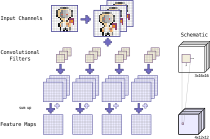
\includegraphics[width=0.6\textwidth]{./4_nn/figs/nn_theory_cnn_basics.eps}
  \caption{Basic CNN layer with a $16 \times 16$ input image, decomposed in 3 channels (CYM) and 4 output feature maps. Kernel size is $5 \times 5$ and the stride is $1$.}
  \label{fig:nn_theory_cnn_basics}
\end{figure}
\FloatBarrier
\noindent


% --
% loss functions

\subsection{Loss Functions and Softmax}
Loss functions or also called cost functions are used to calculate the difference between the predicted labels $\hat{y}$ compared to the actual or ground truth labels $y$.
The predicted labels are usually presented by the output nodes in the last layer of a neural network.
Therefore $\hat{y} = [\hat{y_1}, \, \hat{y_2}, \dots, \hat{y_c}]^T$ has the dimension of the number of labels or classes $c$.
Often it is preferred that $\hat{y} \in R^c$ provides a probability distribution such that:
\begin{equation}
  \sum_{i=0}^c \hat{y}_i = 1
\end{equation}
which can be achieved with the softmax function:
\begin{equation}\label{eq:nn_theory_softmax}
  \hat{y}_i = \frac{\exp{x_i}}{\sum_{j=0}^{c}\exp{x_j}}
\end{equation}
where $c$ is the amount of nodes in this layer, if it is the last layer as usual for the softmax, $c$ is the amount of classes and $\hat{y}_i$ the probability value of the corresponding class $i$.


% --
% dropout

\subsection{Dropout}
Dropout is a method to improve generalization and training of neural network.
The idea is to set the output of randomly selected nodes within a layer and for one training step to zero, so that only the other nodes are updated.
This can be simply done by multiplying all outputs of a current layer with a vector containing a number of zeros and ones places at random positions within the vector.
The amount of zeros compared to ones can be determined by a probability value, for instance $p=0.2$ means that there are 20\% zeros and 80\% ones within the vector.


% --
% training

\subsection{Training of a Neural Network}
The training process of a neural network is usually done with backpropagation of gradients from a loss function at the output nodes.
The backpropagation algorithm is not described here, because there exists many books and papers such as ... with good formulations, further it does not add any value to this thesis as the algorithm is run in the background of all neural network frameworks.
The interesting elements are therefore only the neural network architecture and the loss functions.


% architectures
% --
% Neural Network Architectures

\section{Neural Network Architectures}\label{sec:nn_arch}
\thesisStateRevised
All neural network architectures evaluated on the KWS task of speech commands are presented here.
The fundamental neural network architecture types were:
\begin{enumerate}
	\item CNNs
	\item GANs
	\item Wavenets
\end{enumerate}
CNNs were used for the classification of  MFCC features and are therefore the main architecture type within this thesis.
Generative models, such as GANs, were evaluated in regards of their ability to generate samples from the data distribution.
Further the trained weights from the convolutional layers were applied as pre-trained weights for initialization purpose of a CNN networks with the same convolutional layer structure.
A completely different approach, to the KWS task, was the evaluation of Wavenets operating on raw audio samples as input features.
Deployed in an online system, the Wavenet architecture has no need to extract MFCC features, however it will be shown, that the overall computations are not reduced, because the complexity of Wavenets require many operations.

The amount of parameters and operations are provided for each architecture, to give a comparison between the used models in regards of their computational footprint.


% --
% CNNs

\subsection{Convolutional Neural Networks}\label{sec:nn_arch_cnn}
Three different CNN designs were evaluated, with focus on the striding (shifting) properties of the convolutional filters.
The \texttt{conv-fstride} model has a kernel size adjusted to the length of the frame (time) dimension of the input features and is therefore striding only in the cepstral (frequency) dimension.
In contrast the \texttt{conv-jim} model has a kernel size adjusted to the feature dimension and therefore strides only in the frame (time) dimension.
Also one traditional model named \texttt{conv-trad} is used, that does the striding of convolutional filters in both dimensions.
The summary of the models is presented as follows:
\begin{itemize}
	\item \texttt{conv-trad}: from \cite{Sainath2015} a traditional CNN network, striding in both dimensions.
	\item \texttt{conv-fstride}: from \cite{Sainath2015} (fstride4), striding only in frequency dimension.
	\item \texttt{conv-jim}: self designed model, striding only in frame dimension.
\end{itemize}
The naming of the \texttt{conv-trad} and \texttt{conv-fstride} comes from their original papers, the self defined network \texttt{conv-jim} was named bluntly after the astronaut avatar, that is used for the deployed video game.
The network architecture of the traditional network (\texttt{conv-trad}) is shown in \rfig{nn_arch_cnn_trad}.
% conv-trad
\begin{figure}[!ht]
  \centering
    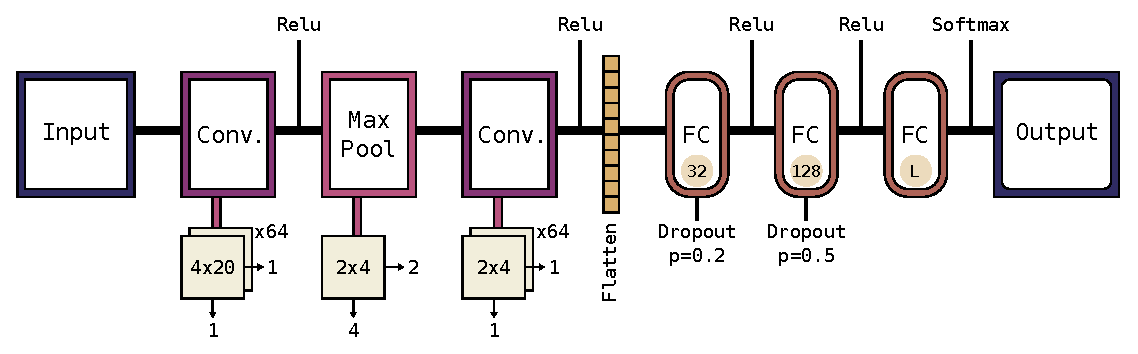
\includegraphics[height=0.2\textwidth]{./4_nn/figs/nn_arch_cnn_trad.eps}
  \caption{Traditional CNN network design from \cite{Sainath2015} named \texttt{conv-trad}.}
  \label{fig:nn_arch_cnn_trad}
\end{figure}
\FloatBarrier
\noindent
The \texttt{conv-trad} network consists of 2 convolutional layers and one max pooling layer in between.
The architecture was adapted from \cite{Sainath2015} as a baseline network and modified a bit in the kernel sizes, so that also reduced input features, for instance 12 MFCCs instead of 39 MFCC (including deltas and energies), can be computed with the same model.
The length of 20 frames in the first convolutional layer is reasonable and corresponds approximately to the length of a vowel sound.
Note that the \enquote{Flatten} layer simply flattens the output tensor of the last convolutional layers to 1-dimension, so that consecutive fully-connected (FC) layers can be appended.
Dropout was used in the first two FC layers to improve generalization.
The last FC layer has $L$ nodes corresponding to $L$ output class labels, depending on the amount of chosen key words in the vocabulary.
Assuming that the input will be of shape $d_x = (1 \times 12 \times 50)$, the following dimensions, amount of parameters and operations for each layer are listed in \rtab{nn_arch_cnn_trad}.
\begin{table}[ht!]
\small
\begin{center}
\caption{Network footprint of \texttt{conv-trad} with 12 output labels.}
\begin{tabular}{ M{1.5cm} M{1.4cm} M{1.2cm} M{1.2cm} M{2cm} M{1.8cm} M{2.3cm} }
\toprule
 \textbf{layer types} & \textbf{number of feature maps} & \textbf{kernel size} & \textbf{stride} & \textbf{output dimension} & \textbf{number of parameters} & \textbf{number of operations}\\
\midrule
input & - & - & - & $1 \times 12 \times 50$ & - & -\\
conv. & 64 & $(4 \times 20)$ & $(1, 1)$ & $64 \times 9 \times 31$ & \num{5184} & \SI{2874.82}{\kilo\ops}\\
max pool & - & $(2 \times 4)$ & $(2, 4)$ & $64 \times 4 \times 7$ & - & -\\
conv. & 64 & $(2 \times 4)$ & $(1, 1)$ & $64 \times 3 \times 4$ & \num{32832} & \SI{835.58}{\kilo\ops}\\
flatten & - & - & - & $1 \times 768$ & - & - \\
fc & - & - & - & $1 \times 32$ & \num{24608} & \SI{49.18}{\kilo\ops} \\
fc & - & - & - & $1 \times 128$ & \num{4224} & \SI{8.32}{\kilo\ops} \\
fc & - & - & - & $1 \times 12$ & \num{1548} & \SI{3.08}{\kilo\ops} \\
\midrule
\textbf{sum} & - & - & - & - & \textbf{\num{68396}} & \textbf{\SI{3770.98}{\kilo\ops}} \\ 
\bottomrule
\label{tab:nn_arch_cnn_trad}
\end{tabular}
\end{center}
\vspace{-4mm}
\end{table}
\FloatBarrier
\noindent

The \texttt{conv-fstride} has the kernel size adapted to the input frame size and is therefore striding only in the frequency dimension.
The kernel height of 8 with vertical stride of 4 creates only two dimensions in the vertical direction for an input size of $(1 \times 12 \times 50)$, which is very energy efficient.
The model is shown in \rfig{nn_arch_cnn_fstride} and its footprint is listed in \rtab{nn_arch_cnn_fstride}
\begin{figure}[!ht]
  \centering
    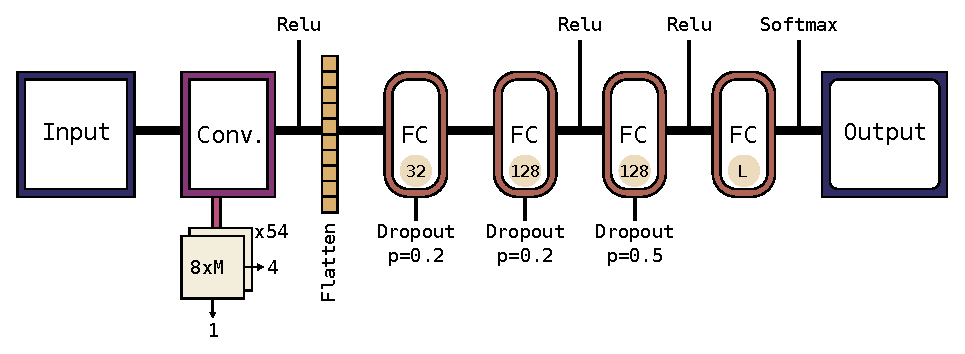
\includegraphics[height=0.2\textwidth]{./4_nn/figs/nn_arch_cnn_fstride.eps}
  \caption{Frequency striding CNN design from \cite{Sainath2015} named \texttt{conv-fstride}.}
  \label{fig:nn_arch_cnn_fstride}
\end{figure}
\FloatBarrier
\noindent
\begin{table}[ht!]
\small
\begin{center}
\caption{Network footprint of \texttt{conv-fstride} with 12 output labels.}
\begin{tabular}{ M{1.5cm} M{1.4cm} M{1.2cm} M{1.2cm} M{2cm} M{1.8cm} M{2.3cm} }
\toprule
 \textbf{Layer Types} & \textbf{Number of Feature Maps} & \textbf{Kernel Size} & \textbf{Stride} & \textbf{Output Dimension} & \textbf{Number of Parameters} & \textbf{Number of Operations}\\
\midrule
input & - & - & - & $1 \times 12 \times 50$ & - & -\\
conv. & 54 & $(8 \times 50)$ & $(4, 1)$ & $54 \times 2 \times 1 $ & \num{21654} & \SI{86.51}{\kilo\ops}\\
flatten & - & - & - & $1 \times 108$ & - & - \\
fc & - & - & - & $1 \times 32$& \num{3488} & \SI{6.94}{\kilo\ops} \\
fc & - & - & - & $1 \times 128$& \num{4224} & \SI{8.32}{\kilo\ops} \\
fc & - & - & - & $1 \times 128$& \num{16512} & \SI{32.90}{\kilo\ops} \\
fc & - & - & - & $1 \times 12$& \num{1548} & \SI{3.08}{\kilo\ops} \\
\midrule
\textbf{sum} & - & - & - & - & \textbf{\num{47426}} & \textbf{\SI{137.75}{\kilo\ops}} \\ 
\bottomrule
\label{tab:nn_arch_cnn_fstride}
\end{tabular}
\end{center}
\vspace{-4mm}
\end{table}
\FloatBarrier
\noindent

The self designed \texttt{conv-jim} consists of two convolutional layers, where the first has an adaptive kernel size in the feature (frequency) dimension and is therefore striding only in frame (time) dimension.
The kernel width of the first convolutional filters is set to $20$, which illustrates much of the learned data structure in the feature maps after the training.
The second convolutional filter has a width of $5$ intended for temporal variations.
The \texttt{conv-jim} model is shown in \rfig{nn_arch_cnn_conv-jim} with footprint in \rtab{nn_arch_cnn_jim}.
\begin{figure}[!ht]
  \centering
    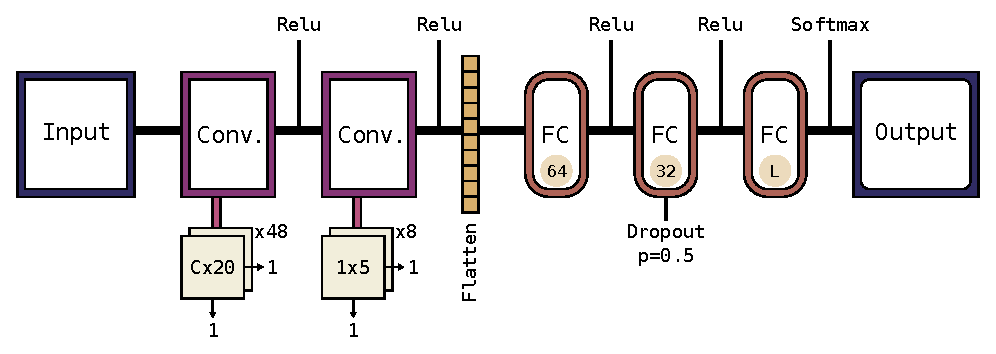
\includegraphics[height=0.2\textwidth]{./4_nn/figs/nn_arch_cnn_conv-jim.eps}
  \caption{Self designed frame (time) striding CNN named \texttt{conv-jim}.}
  \label{fig:nn_arch_cnn_conv-jim}
\end{figure}
\FloatBarrier
\noindent
\begin{table}[ht!]
\small
\begin{center}
\caption{Network footprint of \texttt{conv-jim} with 12 output labels.}
\begin{tabular}{ M{1.5cm} M{1.4cm} M{1.2cm} M{1.2cm} M{2cm} M{1.8cm} M{2.3cm} }
\toprule
 \textbf{layer types} & \textbf{number of feature maps} & \textbf{kernel size} & \textbf{stride} & \textbf{output dimension} & \textbf{number of parameters} & \textbf{number of operations}\\
\midrule
input & - & - & - & $1 \times 12 \times 50$ & -\\
conv. & 48 & $(8 \times 50)$ & $(1, 1)$ & $48 \times 1 \times 31 $ & \num{11520} & \SI{715.73}{\kilo\ops}\\
conv. & 8 & $(8 \times 50)$ & $(1, 1)$ & $8 \times 1 \times 27 $ & \num{1920} & \SI{114.05}{\kilo\ops}\\
flatten & - & - & - & $1 \times 216$ & - \\
fc & - & - & - & $1 \times 64$ & \num{13888} & \SI{27.71}{\kilo\ops} \\
fc & - & - & - & $1 \times 32$ & \num{2080} & \SI{4.13}{\kilo\ops} \\
fc & - & - & - & $1 \times 12$ & \num{396} & \SI{0.78}{\kilo\ops} \\
\midrule
\textbf{sum} & - & - & - & - & \textbf{\num{29804}} & \textbf{\SI{862.40}{\kilo\ops}} \\ 
\bottomrule
\label{tab:nn_arch_cnn_jim}
\end{tabular}
\end{center}
\vspace{-4mm}
\end{table}
\FloatBarrier
\noindent

Note that computational footprint of all three CNN models are different.
The model with the lowest amount of computations, is the \texttt{conv-fstride} model, because of its stride of 4.
The second lowest footprint is given by the \texttt{conv-jim} model.
The \texttt{conv-trad} model requires the highest amount of computations.


% --
% GANs

\subsection{Generative Adversarial Neural Networks}\label{sec:nn_arch_adv}
GANs, as already mentioned in \rsec{prev_nn_adv} and \rsec{nn_theory_gan} are consisting of two separate neural network architectures, denoted as Discriminator (D) and Generator (G) network.
Being able to transfer the obtained weights from the training of the adversarial models, the target layer parameters of the receiving network must coincide with the adversarial network layer parameters.
This implies, that the kernel size of the filters must be equal for each layer, the amount of feature maps must not necessarily be the same.
The convolutional layer parameters of both D and G can be applied for transferring its weights, even if G performs a convolutional upsampling (transposed convolution) instead of a usual convolution, however it is preferred to use a normalization technique, such as frame-based normalization for the G network, otherwise the transferring of weights might be disadvantageous for the classification network.

The only GAN model used for adversarial pre-training has the same convolutional layer structure as the \texttt{conv-jim} network and is therefore denoted as \texttt{adv-d-jim} for the Discriminator model and \texttt{adv-g-jim} for the Generator model, both are shown in \rfig{nn_arch_adv_d_jim} and \rfig{nn_arch_adv_g_jim} respectively.
\begin{figure}[!ht]
  \centering
    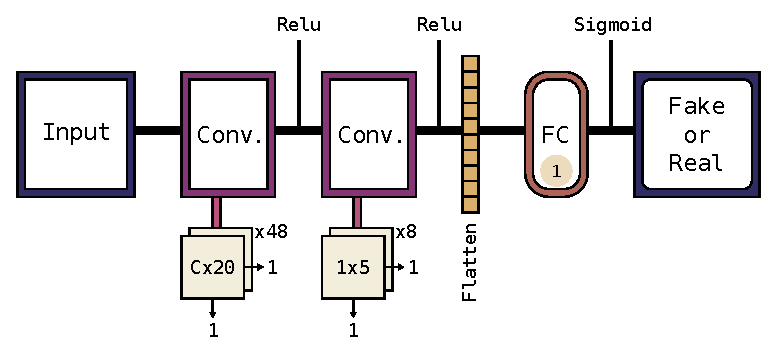
\includegraphics[height=0.2\textwidth]{./4_nn/figs/nn_arch_adv_d_jim.eps}
  \caption{Discriminator model named \texttt{adv-d-jim}.}
  \label{fig:nn_arch_adv_d_jim}
\end{figure}
\FloatBarrier
\noindent
\begin{figure}[!ht]
  \centering
    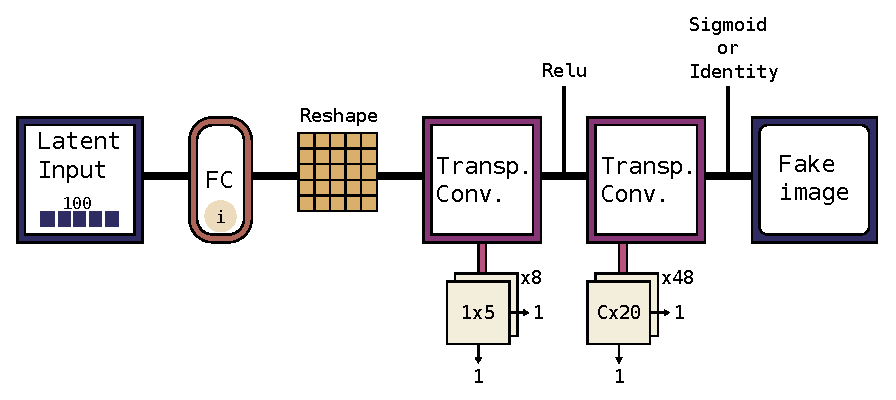
\includegraphics[height=0.23\textwidth]{./4_nn/figs/nn_arch_adv_g_jim.eps}
  \caption{Generator model named \texttt{adv-g-jim}.}
  \label{fig:nn_arch_adv_g_jim}
\end{figure}
\FloatBarrier
\noindent
Note that the number of operations are the same as in \rtab{nn_arch_cnn_jim}, except for the fully-connected layers.
The \texttt{adv-g-jim} model uses either the sigmoid or an identity (same output as input) activation function, depending whether the MFCC are frame-based normalized or not.
If the MFCCs are frame-based normalized, the sigmoid activation function is used to produce outputs in the range of $[0, 1]$, which enhances the model training speed, since the Generator model is able to produce convincing fakes sooner.


% --
% wavenets

\subsection{Wavenets}\label{sec:nn_arch_wavenet}
Wavenets, as introduced in \cite{Oord2016}, were intended for speech generation due to the processing of raw audio data.
In the paper it is mentioned, that Wavenets can be used for ASR tasks as well, though it is very sparsely described.
An implementation of a Wavenet can be found in \cite{Herrmann2018} (without class predictions) and motivated the following model structure.
A Wavenet residual block with an extension for class prediction is illustrated in \rfig{nn_arch_wavenet_block}.
\begin{figure}[!ht]
  \centering
    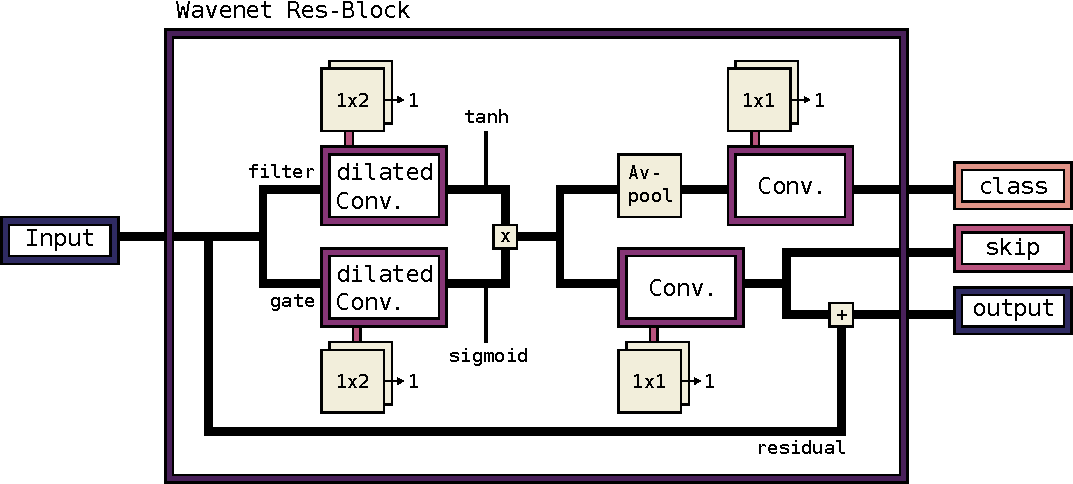
\includegraphics[width=0.7\textwidth]{./4_nn/figs/nn_arch_wavenet_block.eps}
  \caption{Wavenet residual block \cite{Oord2016} with an extension of class prediction layers.}
  \label{fig:nn_arch_wavenet_block}
\end{figure}
\FloatBarrier
\noindent
It is important to note, that the convolutional layers in the residual blocks should not use a bias term, where bias terms led to bad training results in the experiments.
The average filter has a window size of 160 samples and a stride of 80 samples.
One residual block incorporates few parameters, but a huge amount of operations as listed in \rtab{nn_arch_wavenet_block}.
\begin{table}[ht!]
\begin{center}
\caption{Residual block of a Wavenet architecture with extension of class predictions and input sample length of 8000.}
\begin{tabular}{ M{1.5cm} M{1.5cm} M{1.4cm} M{1.4cm} M{2cm} M{2.5cm} M{2.5cm} }
\toprule
 \textbf{layer types} & \textbf{number of feature maps} & \textbf{kernel size} & \textbf{stride} & \textbf{output dimension} & \textbf{number of operations}\\
\midrule
input & - & - & - & $1 \times 8000$ & -\\
conv. gate & 16 & $(1 \times 2)$ & $(1, 1)$ & $16 \times 1 \times 8000 $ & \SI{715.73}{\kilo\ops}\\
conv. filter & 16 & $(1 \times 2)$ & $(1, 1)$ & $16 \times 1 \times 8000 $ & \SI{715.73}{\kilo\ops}\\

\midrule
\textbf{sum} & - & - & - & - & \textbf{\SI{862.40}{\kilo\ops}} \\ 
\bottomrule
\label{tab:nn_arch_wavenet_block}
\end{tabular}
\end{center}
\vspace{-4mm}
\end{table}
\FloatBarrier
\noindent
Note that the dilated convolutional filters have a filter size of two with adjustable dilation parameter and that strides are merely done in the time dimension, because the input is a one-dimensional time signal.
The $1 \times 1$ convolutions are a special type of convolutional filters and work in the same manner as usual convolutions, just with a filter size of one. 
The whole Wavenet architecture is composed of several consecutive Wavenet residual blocks with increasing dilation parameters for the first two convolutional layers (filter and gate) in the blocks.
The whole Wavenet architecture adaption with class prediction is shown in \rfig{nn_arch_wavenet_all}.
\begin{figure}[!ht]
  \centering
    \includegraphics[width=0.9\textwidth]{./4_nn/figs/nn_arch_wavenet_all.eps}
  \caption{Whole Wavenet architecture with class prediction extension.}
  \label{fig:nn_arch_wavenet_all}
\end{figure}
\FloatBarrier
\noindent
Note that the last convolutional layer for the sample prediction has a total amount of feature maps ($1 \times 256$) selected to the quantized audio representation of 256 possible values.
More details about the used quantization technique is described in \cite{Oord2016}.
The computational footprint of the whole Wavenet model is listed in \rtab{nn_arch_wavenet_whole}.
\begin{table}[ht!]
\small
\begin{center}
\caption{Whole Wavenet architecture with extension of a class predictions of 12 output labels and input sample length of \num{8000}.}
%\begin{tabular}{ M{2cm} M{1.5cm} M{1.2cm} M{1.2cm} M{2cm} M{1.5cm} M{2.3cm} }
\begin{tabular}{ M{1.5cm} M{1.4cm} M{1.1cm} M{1.1cm} M{2cm} M{1.5cm} M{2.6cm} }
\toprule
 \textbf{Layer Types} & \textbf{Number of Feature Maps} & \textbf{Kernel Size} & \textbf{Stride} & \textbf{Output Dimension} & \textbf{Number of Parameters} & \textbf{Number of Operations}\\
\midrule
input & - & - & - & $1 \times 8000$ & - & -\\
7 res. blocks & - & - & - & - & \num{14896} & \SI{19453.98}{\kilo\ops}\\
conv. s1 & 2 & $(1 \times 1)$ & $(1, 1)$ & $1 \times 1 \times 8000$ & \num{4} & \SI{48.00}{\kilo\ops} \\
conv. s2 & 256 & $(1 \times 1)$ & $(1, 1)$ & $256 \times 1 \times 8000$ & \num{768} & \SI{12288.00}{\kilo\ops} \\
conv. c1 & 128 & $(1 \times 1)$ & $(1, 1)$ & $1 \times 1 \times 99$ & \num{16512} & \SI{4866.05}{\kilo\ops} \\
conv. c2 & 1 & $(1 \times 1)$ & $(1, 1)$ & $1 \times 1 \times 99$ & \num{129} & \SI{38.02}{\kilo\ops} \\
fc & - & - & - & $1 \times 12$ & \num{1200} & \SI{2.39}{\kilo\ops} \\
\midrule
\textbf{sum} & - & - & - & - & \textbf{\num{33509}} & \textbf{\SI{36695.02}{\kilo\ops}} \\
\bottomrule
\label{tab:nn_arch_wavenet_whole}
\end{tabular}
\end{center}
\vspace{-4mm}
\end{table}
\FloatBarrier
\noindent
The amount of operations are quite large, because the convolutional filters have to be applied on each sample of the audio signal and no concatenation is used apart from the added class prediction layers with an average filter.

% adversarial
% --
% adversarial

\section{Adversarial Pre-Training}\label{sec:nn_adv}
\thesisStateRevised
In adversarial neural network training, two separate neural networks are competing against each other in an adversary task.
This competition of the two networks motivates them to improve their performance and beat the other network.
The application of GANs, as already explained in \rsec{prev_nn_adv} and \rsec{nn_theory_gan}, is an interesting subject in research and the questions whether the obtained weights from the training of the Generator (G) and Discriminator (D) network can contribute to better the performances in equivalent models, arises.
In the following the training algorithms are explained in more detail, such as the loss functions used for G and D.
The transfer of weights can be done for training instances on small subsets of labels or the whole network by regarding all labels at once in a single training instance.
%The transferring technique of the whole network is denoted as adversarial dual train and the training of separate labels is named adversarial label train.
The transferring technique of training instances on small subsets of labels is denoted as adversarial label train and the transfer of weights from a whole network with all labels is named as adversarial dual train.
In the following those training techniques are further explained, except of the adversarial dual train, because it is straight forward if the adversarial label train is explained.

% --
% training GANs

\subsection{Training Generative Adversarial Neural Networks}
The interesting part in training GANs is how the Generator (G) and Discriminator (D) models are updated in each training step and which loss functions were used.
In \req{nn_theory_gan} the game is notated as min-max game, from which the loss of D $l_D$ can be described for one specific training example $i$ of a batch as:
\begin{equation}
  l_D(x_i, z_i, G) = l(D(x_i), y_r) + l(D(G(z_i)), y_f)
\end{equation}
where $l$ is the binary cross-entropy loss described in \req{nn_theory_binary_cross_entropy}, $D: \mathcal{X} \mapsto [0, 1]$ and $G: \mathcal{Z} \mapsto \mathcal{X}$, $x_i \in \mathcal{X}$ is the data example, $z_i \in \mathcal{Z}$ is a randomly sampled latent variable, $y_r = 1$ is the real label and $y_f = 0$ the fake label for that specific example $i$.
In contrast the loss of the Generators $l_G$ is:
\begin{equation}
  l_G(z_i, D) =  l(D(G(z_i)), y_r)
\end{equation}
with $y_r$ as real label to perform maximization of $\log D(G(\bm{z}))$ as described in \rsec{nn_theory_gan}.
An extended approach, so that G produces samples specifically similar to the data distribution and does not drift off into creating unrealistic fakes of noisy samples to fake D, is to incorporate a similarity term with the \emph{cosine similarity}:
\begin{equation}
  s(\bm{x_1}, \bm{x_2}) = \frac{\bm{x_1}^T \bm{x_2}}{\norm{\bm{x_1}}_2 \cdot \norm{\bm{x_2}}_2 + \epsilon} 
\end{equation}
where $s : (\mathcal{X}, \mathcal{X}) \mapsto [0, 1]$ is the cosine similarity function, $\bm{x_1}$ and $\bm{x_2}$ are two vectors for similarity measure and $\epsilon$ is a small number, such that no division by zero is possible.
With the similarity loss incorporated, $l_G$ gets:
\begin{equation}
  %l_G(x_i, z_i, D) =  l(D(G(z_i)), y_r) + \lambda (1 - \E \left[ s(x_i \bm{e}, G(z_i)) \right])
  l_G(x_i, z_i, D) =  l(D(G(z_i)), y_r) + \lambda \left(1 - \frac{1}{C} \sum_{c=0}^{C} s(\hat{\bm{e}}_c^T x_i , \hat{\bm{e}}_c^T G(z_i)) \right)
\end{equation}
where $\hat{\bm{e}}_c \in \{1, 0\}^C$ is a unit vector representing one cepstral coefficient of the Mel Frequency Cepstral Coefficient (MFCC) data $x_i \in \mathcal{X} = \R^{C \times M}$ with a total number of $C$ MFCC coefficients and $M$ frames.
Further $\lambda$ is a trade-off factor between data similarity and fake loss from D.
For the experiments in \rsec{exp_adv}, $\lambda = 5$ was chosen.

The update of D and G can be done for each training step by backpropagating the obtained losses.
However it is more appealing if D is updated for a certain numbers of training steps with no update of G and then alternating to updates of G without updating D.
This will give either D or G some update steps to improve in their specific adversarial task of either discriminating or generating.
In this thesis the training steps for updating either D or G was selected to 2 epochs.
Note that an epoch consists of several training steps depending on the batch size and amount of data, this can vary for the experiments, however it does not influence that much on the overall end results.


% --
% label train

\subsection{Adversarial Label Train}
Adversarial label train, is the transfer of weights from feature maps trained on multiple GAN training instances on subsets of all labels.
For instance if the total amount of labels are \{\enquote{left}, \enquote{right}\} then an own training instance can focus on the label \enquote{left} and another on the label \enquote{right}.
It is important to assign a specific number of feature maps to each label train instance, for example each label train gets 8 feature maps of the first convolutional layers.
The label train scheme is illustrated in \rfig{nn_adv_label_scheme} and applies 6 label train instances, such as used for the experiments in \rsec{exp_adv}.
\begin{figure}[!ht]
  \centering
    \includegraphics[width=0.7\textwidth]{./4_nn/figs/nn_adv_label_scheme}
  \caption{Label train scheme of 6 training instances, trained with 100 epochs for each label subset.}
  \label{fig:nn_adv_label_scheme}
\end{figure}
\FloatBarrier
\noindent
An actual GAN training for the labels \enquote{left} and \enquote{go} is shown in \rfig{nn_adv_loss_label}.
Note that the update of either the Discriminator (D) or Generator (G) model is done alternating for 2 training epochs.
\begin{figure}[!ht]
  \centering
  \subfigure[it-100]{\includegraphics[width=0.45\textwidth]{./4_nn/figs/nn_adv_loss_label_it-100}}
  \subfigure[it-1000]{\includegraphics[width=0.45\textwidth]{./4_nn/figs/nn_adv_loss_label_it-1000}}
  \caption{Adversarial training loss of the labels \enquote{left} and \enquote{go} with 8 feature maps.}
  \label{fig:nn_adv_loss_label}
\end{figure}
\FloatBarrier
\noindent
The creation of fake images from G is shown in \rfig{nn_adv_fakes_label} of the same training instances.
\begin{figure}[!ht]
  \centering
  \subfigure[it-100]{\includegraphics[width=0.45\textwidth]{./4_nn/figs/nn_adv_fakes_label_it-100}}
  \subfigure[it-1000]{\includegraphics[width=0.45\textwidth]{./4_nn/figs/nn_adv_fakes_label_it-1000}}
  \caption{Generation of fake images of the labels \enquote{left} and \enquote{go} with 8 feature maps for the GAN training.}
  \label{fig:nn_adv_fakes_label}
\end{figure}
\FloatBarrier
\noindent

As showcase example, some concatenated adversarial label train weights used for weight transfer, are shown for D and G with different amounts of training epochs in \rfig{nn_adv_label_weights_d} and \rfig{nn_adv_label_weights_g}.
\begin{figure}[!ht]
  \centering
  \subfigure[d-100]{\includegraphics[width=0.45\textwidth]{./4_nn/figs/nn_adv_label_weights_d-100}}
  \subfigure[d-1000]{\includegraphics[width=0.45\textwidth]{./4_nn/figs/nn_adv_label_weights_d-1000}}
  \caption{Concatenated label weights of the first convolutional layer from the Discriminator model with different amounts of epochs.}
  \label{fig:nn_adv_label_weights_d}
\end{figure}
\FloatBarrier
\noindent
\begin{figure}[!ht]
  \centering
  \subfigure[g-100]{\includegraphics[width=0.45\textwidth]{./4_nn/figs/nn_adv_label_weights_g-100}}
  \subfigure[g-1000]{\includegraphics[width=0.45\textwidth]{./4_nn/figs/nn_adv_label_weights_g-1000}}
  \caption{Concatenated label weights of the first convolutional layer from the Generator model with different amounts of epochs.}
  \label{fig:nn_adv_label_weights_g}
\end{figure}
\FloatBarrier
\noindent
The amounts of epochs are important, because they determine how much the models are learning in their adversarial task.
With 100 epochs the Generator creates similar feature maps for each label train instance, because it does not need to be that accurate in creating different looking fakes, however the Discriminator gets better as well and the need of generating different looking fakes are necessary to match up.
With 1000 epochs the Generator produces already different fakes as already shown in \rfig{nn_adv_fakes_label} however it is not recommended to train for too long.
Note that a second convolutional layer for the \texttt{adv-d-jim} and \texttt{adv-g-jim} exist as well, the corresponding weights are shown only for the 100 epoch examples in \rfig{nn_adv_label_weights_conv1}.
\begin{figure}[!ht]
  \centering
  \subfigure[d-100]{\includegraphics[width=0.25\textwidth]{./4_nn/figs/nn_adv_label_weights_conv1_d-100}}
  \qquad \qquad
  \subfigure[g-100]{\includegraphics[width=0.25\textwidth]{./4_nn/figs/nn_adv_label_weights_conv1_g-100}}
  \caption{Concatenated label weights of the second convolutional layer from the Discriminator and Generator model with trained with 100 epochs.}
  \label{fig:nn_adv_label_weights_conv1}
\end{figure}
\FloatBarrier
\noindent
From the second convolutional layer each row corresponds to a single feature map and therefore 8 rows to one adversarial label training instance.
% \subsection{Questions that arise}
% There are several questions that arise regarding Adversarial Training:
% \begin{enumerate}[label={Q.\textgoth{A}.\arabic*)}, leftmargin=1.4cm]
%   \item Does the Network Architecture of G and D have to be the same but transposed?
%   \item Does the value space of in and outputs, for D and G respectively, have to be limited between a range of [0, 1] done by for instance the frame normalization, or sigmoid output?
%   \item What loss function works well for training?
%   \item How long should be trained?
%   \item When transfering weights to another network, should the weights from G or D be transfered?
%   \item Does the classification network has to adapt the parameters from the transfered weights?
%   \item Whats the benefit of all this?
% \end{enumerate}

% To illustrate the idea an example is shown of the labels L5 (left, right, up, down, go).

% The convolutional layer weights from the adversarial training of the individual labels, 
% can be stacked together an used to initialize another network.
% An example of this method is shown in \rfig{nn_adv_example}, where the initialization pattern changes to more elaborate structures and patterns to form good classification outputs. 
% However the Basic Pattern from the adversarial training stays the same, which is a good sign, because then the network is accepting those trained weights and adapts them.

% \begin{figure}[!ht]
%   \centering
%     \subfigure[c1 trained]{\includegraphics[width=0.45\textwidth]{./4_nn/figs/nn_adv_example_c0}}
%     \subfigure[c1 init]{\includegraphics[width=0.45\textwidth]{./4_nn/figs/nn_adv_example_c0_init}}
%     \subfigure[c2 trained]{\includegraphics[height=0.45\textwidth]{./4_nn/figs/nn_adv_example_c1}}
%     \quad
%     \subfigure[c2 init]{\includegraphics[height=0.45\textwidth]{./4_nn/figs/nn_adv_example_c1_init}}
%   \caption{Adversarial Training Example: Convolutional layers pretrained with adversarial training on each label separately.}
%   \label{fig:nn_adv_example}
% \end{figure}
% \FloatBarrier
% \noindent

% For this example in adversarial training, 8 feature maps of the first layer were used for each label, also they belong to the Generator Network G or decoder (dec). In Convolutional Networks, each previous layers feature map creates a new set of feature maps in the next layer.
% An example of this label training is shown in \rfig{nn_adv_example_label} with feature maps [(1, 8), (8, 8)] of the convolutional layers

% \begin{figure}[!ht]
%   \centering
%     \subfigure[\enquote{left} c1 from D]{\includegraphics[width=0.45\textwidth]{./4_nn/figs/nn_adv_example_label_left_c0_enc}}
%     \subfigure[\enquote{left} c1 from G]{\includegraphics[width=0.45\textwidth]{./4_nn/figs/nn_adv_example_label_left_c0_dec}}
%     \subfigure[\enquote{left} c2 from D]{\includegraphics[width=0.3\textwidth]{./4_nn/figs/nn_adv_example_label_left_c1_enc}}
%     \subfigure[\enquote{left} c2 from G]{\includegraphics[width=0.3\textwidth]{./4_nn/figs/nn_adv_example_label_left_c1_dec}}
%   \caption{Adversarial Training example of Generator (G) and Discriminator (D) of label \enquote{left} captured with 8 feature maps of the first convolutional layer.}
%   \label{fig:nn_adv_example_label}
% \end{figure}
% \FloatBarrier
% \noindent

% Those trained weights from each label can then simply be put into the feature maps of a classification network.
% This is shown in \rfig{nn_adv_example} where c1 from G and c2 from G in \rfig{nn_adv_example_label} were transfered to the first row(s).
% When doing the transferring of feature maps, it is important that the layers are not mixed up so that the trained connections are still correct.
% Also of course the weights of the feature maps must have the same dimension, so that transferring is possible.


% \subsection{Observing the Generators output}
% While the output of the Discriminator is rather uninteresting (one-dimensional probability value), the output of the Generator is a good indicator of how well the training between D and G has gone.
% Optimally the output of the Generator look like real data samples.
% An example of a trained Generator Network with fake outputs compared to real ones is shown in \rfig{nn_adv_gen}.

% \begin{figure}[!ht]
%   \centering
%     \subfigure[\enquote{left} real examples]{\includegraphics[width=0.45\textwidth]{./4_nn/figs/nn_adv_gen_left_real}}
%     \subfigure[\enquote{left} fakes from G]{\includegraphics[width=0.45\textwidth]{./4_nn/figs/nn_adv_gen_left_fake}}
%   \caption{Real samples of \enquote{left} from the Speech Commands dataset compared to fake samples from a trained Generator Network.}
%   \label{fig:nn_adv_gen}
% \end{figure}
% \FloatBarrier
% \noindent

% If the fake example of the Generator Network do not look similar to real ones, then something might have gone wrong in the training between the Generator and Discriminator Network.
% Further it can be evaluated if a certain network architecture is able to produce a label in a sufficient representation, therefore this method might be a good start in finding a suitable network architecture for the problem to be solved.




% --
% Experiments

\chapter{Experiments}\label{sec:exp}
All experiments performed on the speech command datasets with their obtained results are presented in this chapter.
The speech command datasets are described and analyzed in detail.
Samples from those datasets with their feature extracted representation are shown and the quality and diversity of the recordings is discussed.
The experiments were run on the neural network architectures presented in \rsec{nn_arch}.
In detail the experiments include the feature selection of Mel Frequency Cepstral Coefficients (MFCC) evaluated on Convolutional Neural Network (CNN) architectures, to observe the impact of feature reduction and a frame-based normalization.
Further the transfer of weights from trained Generative Adversarial Neural Networks (GAN) to CNN networks is evaluated.
The performance of a Wavenet architecture operating on raw audio samples is examined.

% dataset
% --
% dataset

\section{Dataset}\label{sec:exp_dataset}
This thesis uses two datasets, one is the second version of the speech commands dataset \cite{Warden2018} and the other is self made consisting of only 5 labels (speech commands) that are especially valuable for movement in video games.
The self made dataset is referred to as \enquote{my dataset} and is used as additional evaluation set.
The training, validation, and testing of the neural network architectures performs on the speech commands dataset.
Both datasets consists of raw waveform files in the \texttt{.wav} format without any feature extraction done beforehand.
As already mentioned in \rsec{prev_kws_benchmark}, the direct comparisons between different neural network approaches is difficult, if the feature extraction is left alone to the user.
Some datasets provide feature extraction beforehand so that the comparability of individual neural network architectures performances is not influenced on it.
The speech commands dataset does not explicitly separate each \texttt{.wav} file into train, test, and validation sets, but provides file lists that refer to distinct waveform files that should be used for testing and validation. 
That means, when the same test and validation sets are used in different research projects, it provides means for comparison to the individual researchers.


% --
% speech commands dataset

\subsection{Speech Commands Dataset}\label{sec:exp_dataset_speech_cmd}
The speech command dataset \cite{Warden2018} consists of \SI{1}{\second} speech recordings, done by over thousands of individual speakers and exists in two versions (\texttt{v0.01} and \texttt{v0.02}).
The first version was published in 2017 with a total number of 30 keywords.
In 2018 the second version extended the first version with 5 additional keywords \{\enquote{backward}, \enquote{forward}, \enquote{follow}, \enquote{learn}, \enquote{visual}\}.
Further, more class examples were added and a better quality check was implemented in order to remove poor quality recordings.

In this thesis, the experiments are solely performed on the second version \texttt{v0.02} of the dataset with hard-facts listed in \rtab{exp_dataset_hard_facts}.
\begin{table}[ht!]
\begin{center}
\caption{Hard facts of the speech commands dataset \texttt{v0.02}.}
\begin{tabular}{ M{5cm}  M{2cm} }
\toprule
%\textbf{label} & \textbf{train} \\
%\midrule
Total number of key words & 35\\
Total number of examples & 105886\\
Total number of speakers & 2618\\
\midrule
%Number of core key words & 20\\
%Number of auxiliary key words & 15\\
Recording duration & 0.4 - \SI{1}{\second}\\
Channels & Mono\\
Bit depth of audio files & \SI{32}{\bit}\\
Sampling frequency & \SI{16}{\kilo\hertz}\\
\bottomrule
\label{tab:exp_dataset_hard_facts}
\end{tabular}
\end{center}
\end{table}
\FloatBarrier
\noindent


All available speech command keywords with their separation in training, test, and validation set are shown in \rtab{exp_dataset_all_labels} located in the appendix.
Some keywords have a significantly higher number of examples per class than others.
This inconsistency of examples per classes emerged from the recording settings, as described in \cite{Warden2018}, where the main keywords were recorded with a higher number of examples from the same speaker.
For instance, the same speaker produces five examples of \enquote{go} and two of \enquote{marvin}.
This makes the keywords separable into so called \emph{core keywords} and \emph{auxiliary keywords}.
The core keywords are the main classification objective and each core keyword should correspond to one individual class label.
Therefore the core keywords have the higher count of samples with about 3700 to 4000 examples each.
In detail the core keywords are \{\enquote{yes}, \enquote{no}, \enquote{up}, \enquote{down}, \enquote{left}, \enquote{right}, \enquote{on}, \enquote{off}, \enquote{stop}, \enquote{go}, \enquote{zero}, \enquote{one}, ..., \enquote{nine} \}.

The auxiliary keywords have the purpose to disturb the classification of the core keywords.
Therefore the auxiliary keywords should be labeled separately with one single class label.
In many papers those auxiliary keywords are labeled as \enquote{unknown}.
In this thesis, the label \enquote{\_mixed} presents a mixture of all auxiliary keywords and the core keywords that were not used for classification.
The \enquote{\_mixed} keywords represent all unknown words that an user might speak and are therefore a very important element in the KWS task for the identification of words that are not in the class dictionary.
Note that the \enquote{\_mixed} label makes the classification task much more challenging because the network has to be more accurate in modeling each core keywords against the other core keywords and additionally to the auxiliary keywords.
In the creation of the examples for the \enquote{\_mixed} label, it is preferable to have an equal number of examples per individual auxiliary keyword and unused core keywords.
This was done by placing all unused core keywords and auxiliary words into a separate folder and reading them into an ordered list.
This list is ordered such that one example per keyword is placed consecutively to the next and repeated until all examples were added.
The auxiliary keyword examples picked for training are referenced by the entries of the ordered list, starting from index 0 to the number of training examples per class.

To examine the recorded examples from the speech command dataset, \rfig{exp_dataset_speech_cmd_wav_grid} shows one example from all available speech commands and presents them in raw audio format, where vertical lines indicate the onset detection and end of a \SI{500}{\milli\second} window.
\begin{figure}[!ht]
  \centering
    \includegraphics[width=0.65\textwidth]{./5_exp/figs/exp_dataset_speech_cmd_wav_grid.png}
  \caption{One random sample of each individual speech command in the speech command dataset presented in normalized audio waveform.}
  \label{fig:exp_dataset_speech_cmd_wav_grid}
\end{figure}
\FloatBarrier
\noindent


% --
% statistics

\subsubsection{Observations of all available Examples in the Dataset}
Two histograms were created to observe the quality of all recorded files in the dataset.
Those histograms present an energy measure and a count of the sample length for each file.
The energy of a recorded file provides information about a recordings amplification setting and is an indicator for too silent or too loud (overdrive distortions) samples.
In the first version of the speech command dataset, namely \texttt{v0.01}, the silent files were a problem.
This had been fixed in the second version by rejecting those files.
Therefore, the version \texttt{v0.01} is slightly more unclean than \texttt{v0.02}.
The energy value $e \in \R$ can be computed by
\begin{equation}\label{eq:exp_dataset_energy}
  e = \frac{1}{n} \left( \bm{x}^T \bm{x} \right),
\end{equation}
where $\bm{x} \in \R^n$ represents a single recorded file with a total number of $n$ samples.
The division through the sample length $n$ of each individual audio recording is required because not every file has a duration of \SI{1}{\second} (16000 samples).
For an unknown reason, many of the recordings consist of less than 16000 samples, which would be problematic if the sample length is too short to fully capture a keyword.
So the minimum duration of all examples was determined and found to last about \SI{0.4}{\second}.
This however, is adequate for words like \enquote{go}, where the reduced samples length often shows up.
\rfig{exp_dataset_hist} shows the mentioned histograms of all available examples in the dataset.
\begin{figure}[!ht]
  \centering
    \subfigure[energy measure]{\includegraphics[width=0.42\textwidth]{./5_exp/figs/exp_dataset_hist_energy_overall.png}}
    \qquad
    \subfigure[count of sample length]{\includegraphics[width=0.42\textwidth]{./5_exp/figs/exp_dataset_hist_sample_overall.png}}
  \caption{Histograms of all available examples in the speech commands dataset \texttt{v0.02}, where one histogram shows an energy measure in log-log scale and the other a count of the sample length in log scale.}
  \label{fig:exp_dataset_hist}
\end{figure}
\FloatBarrier
\noindent
The histogram of the energy measure has one main lobe, which implies that there are no clusters of extremely silent or loud files.
For comparison, if silent files were extracted from the given background files, the energy of some of those would be in a range of $10^{-7} \dots 10^{-6}$ indicating that those files are too silent.
The sample length histogram shows that most of the files consist of 16000 samples but many others have a smaller number of samples. 
This is relevant and has to be considered in the pre-processing of audio files because inputs to neural networks often have to be prepared to fixed size inputs if no sequential neural networks, such as RNNs, are used.


% --
% recording quality

\subsubsection{Recording Quality and Personal Experience}
The examples of the speech commands dataset \cite{Warden2018} were not recorded by professionals with high-end recording equipment.
In fact the recordings had been done in an amateur kind of fashion so that the dataset is more suited to realistic environments intended for user applications.
This is also noted in the paper \cite{Warden2018}:
\begin{quote}
...This meant that the use of studio-captured samples seemed unrealistic, since that audio would lack background noise, would be captured with high-quality microphones, and in a formal setting. 
Successful models would need to cope with noisy environments, poor quality recording equipment, and people talking in a natural, chatty way...
\end{quote}
The recording devices of the speakers, who contributed examples to the dataset, were in most cases consumer microphones, as for instance, embedded microphones in laptops or mobile phones.

The conclusions drawn from listening to the examples in the dataset are as follows:
\begin{itemize}
  \item The quality of the examples in the dataset are ranging from excellent and perfectly recognizable to very poor, noisy, unrecognizable, and cut off. Although most of the examples are provided with sufficient quality.
  \item Different accents had been perceived, which suggests that people from several nationalities were involved.
  However, the bias was laid on American English, as noted in the paper.
  \item No children speakers had been found.
\end{itemize}
Due to data privacy issues the information of individual speakers is not displayed.
Therefore, it is not clear whether the dataset consists of an equal amount of male and female speakers and whether there are any children speakers included.
The last would be especially interesting for a video games intended for children.

In many recordings the background noise is imminent, such as traffic noise, chattering people, office sounds, and many more.
A quality check of the recorded files in the dataset had been done beforehand to ensure that poor quality examples are rejected.
Nevertheless, there are still some existing flaws, such as extremely loud or silent recordings, examples with inconsistent sample numbers, recordings that include too much noise or in the worst case noise only (very rarely), and cut off signals capturing only half of a word.
Those quality issues in the dataset can for most cases be neglected or fixed, such as inconsistent sample numbers. 
Other more problematic cases, like noise-only examples, should ideally be removed.
But since their occurrence is very rare it is not worth the effort.
Besides, it is usually not a problem for neural networks to cope with noisy datasets.
In many cases it is favorable when a dataset contains many noisy samples so that neural networks can learn invariance against noise, loudness differences, and other nuisances during training.
Moreover, if the training dataset is sufficiently large, and the test and validation sets do not contain very poor examples, there should be no problem in the training and evaluation of different models.
Finally, it has to be acknowledged that the dataset is published under the creative common license, hence it is freely available to everyone, which is simply fabulous.


% --
% dataset structure

\subsubsection{Dataset Structure}\label{sec:exp_dataset_structure}
The speech command examples are stored in separate folders named after each individual keyword.
The folder named as \texttt{\_background\_noise\_} contains six different background noise files, such as \texttt{white\_noise.wav} or \texttt{doing\_the\_dishes.wav}, with a duration of more than one minute each and altogether summing up to a duration of about \SI{400}{s}.
To extract noise examples from those files with a sufficient number of examples of over 3500, those noise files have to be extracted by a striding window of \SI{1}{\second} length shifted by \SI{0.110}{\second}.
The noise examples were assigned to the label \enquote{\_noise}.

Each waveform file from the keyword folders is named by an 8-digit hexadecimal hash code for the speaker identification and followed by the utterance number, for instance \texttt{3b4f8f24\_nohash\_0.wav}.
With the speaker identification code known it is possible to distinguish between different speakers.
However, as mentioned above, no further information about the speakers is provided due to data privacy issues.

Moreover, the dataset contains a testing file list called \texttt{testing\_list.txt} and a validation file list \texttt{validation\_list.txt}, where each row entry in the text file refers to a file in the dataset, as for example \texttt{right/bb05582b\_nohash\_3.wav}.
Those file lists should ensure the comparability between different neural network approaches from individual researchers.
The testing and validation file lists are applied in this thesis and the separation into sets are shown in \rtab{exp_dataset_all_labels}.


% --
% extracted examples

\subsubsection{Samples from the Feature Extraction}
The feature extracted data examples are stored to separate files before using them for training.
This has the practicability that features do not have to be extracted each time a new training instance of a neural network is performed.
Samples from the extracted MFCCs with frame-based normalization, as explained in \rsec{signal_mfcc}, are shown in \rfig{exp_dataset_speech_cmd_mfcc}.
\begin{figure}[!ht]
  \centering
    \subfigure[left]{\includegraphics[width=0.48\textwidth]{./5_exp/figs/exp_dataset_speech_cmd_mfcc_left.png}}
    \subfigure[right]{\includegraphics[width=0.48\textwidth]{./5_exp/figs/exp_dataset_speech_cmd_mfcc_right.png}}
    \subfigure[up]{\includegraphics[width=0.48\textwidth]{./5_exp/figs/exp_dataset_speech_cmd_mfcc_up.png}}
    \subfigure[down]{\includegraphics[width=0.48\textwidth]{./5_exp/figs/exp_dataset_speech_cmd_mfcc_down.png}}
    \subfigure[go]{\includegraphics[width=0.48\textwidth]{./5_exp/figs/exp_dataset_speech_cmd_mfcc_go.png}}
  \caption{MFCC extraction of randomly selected 30 samples per class label obtained from the training set of the speech commands dataset \texttt{v0.02}. The corresponding class labels are written below the plots.}
  \label{fig:exp_dataset_speech_cmd_mfcc}
\end{figure}
\FloatBarrier
\noindent


% --
% my dataset

\subsection{My Dataset}\label{sec:exp_dataset_my}
This dataset was created by the author of this thesis and contains five examples for each of the following keywords \{\enquote{left}, \enquote{right}, \enquote{up}, \enquote{down} and \enquote{go}\}.
The datasets purpose is mainly to have an additional test set for evaluating trained models on the authors own voice.
The examples per keyword are spoken with different emphasis and stress on individual phonemes for each keyword.
Also the prolongation of the words are different, for instance, in one example the word is spoken very hasty and in the other it is spoken slowly.
The emphasis and prolongation ensure the diversity of the dataset.
It is relevant to mention that none of the self recorded files were used within the training set so that the neural networks performance is evaluated on unseen data.
All examples of \enquote{my dataset} are illustrated in \rfig{exp_dataset_my_wav_grid} in raw audio format.
\begin{figure}[!ht]
  \centering
    \includegraphics[width=0.6\textwidth]{./5_exp/figs/exp_dataset_my_wav_grid.png}
  \caption{Self recorded files of the \enquote{my dataset} in raw audio format.}
  \label{fig:exp_dataset_my_wav_grid}
\end{figure}
\FloatBarrier
\noindent
The same examples extracted to MFCC features are shown in \rfig{exp_dataset_my_mfcc}.
\begin{figure}[!ht]
  \centering
    \includegraphics[width=0.65\textwidth]{./5_exp/figs/exp_dataset_my_mfcc.png}
  \caption{All MFCC extracted samples of the \enquote{my dataset} with the same ordering as shown in \rfig{exp_dataset_my_wav_grid}.}
  \label{fig:exp_dataset_my_mfcc}
\end{figure}
\FloatBarrier
\noindent
It turned out that it is a very hard task for neural networks to achieve a \SI{100}{\percent} classification score upon it, despite the fact that all examples correspond to the same speaker.
This is slightly worrying because acoustically each of the examples per word is perfectly distinguishable for humans.
For instance, in the classification of the five examples of \enquote{left} from the \enquote{my dataset}, the trained models may classify 4 examples as \enquote{left} and one as \enquote{right}.
It is difficult to examine why exactly this single example was wrongly classified.


% --
% preparation for neural networks

\subsection{Data Preparation for Neural Networks}\label{sec:exp_data_prep}
The neural network architectures are trained with supervised learning.
This implies that a class label $y_i \in \{0, 1, \dots, L\}$ correspondence to each data example $x_i \in \mathcal{X}$ exists, where $L$ is the total number of classes and $\mathcal{X}$ is the input space of the data example.
The input space for MFCC features is, for example, $\mathcal{X} = \R^{C \times M}$ with $C$ cepstral coefficients and $M$ frames.
Selected examples including their labels form a set $S$, for example for training or testing, which can be written as
\begin{equation}\label{eq:exp_dataset}
  S = \{ (x_i, y_i) \mid i = 0, 1, \dots, n \},
\end{equation}
where $n$ is the total number of examples within this set.
Class labels $y_i$ are usually translated to integer numbers that are referencing to indices in a class dictionary.
For instance, $y_1 = 0$ of example $i=1$ refers to the label \enquote{left} in the dictionary \{0: \enquote{left}, 1: \enquote{right}\}.
It is essential that the enumeration of class labels in the class dictionary starts from zero because they should correspond to the output nodes in the used neural network.

\rsec{signal_mfcc} already showed how to extract MFCC features.
Nevertheless, it is important that each individual $x_i$ for all $i$ has the same dimension $\mathcal{X}$ so that a data preparation for the training of neural networks is possible.
It could happen that the sample numbers of the waveform files are inconsistent, as described in \rsec{exp_dataset_speech_cmd}, and therefore different dimension of individual data examples may be obtained.
To ensure that all $x_i$ have the same dimension, the audio files were adjusted to the same fixed sample length of a duration of \SI{1}{\second} and sampling frequency \SI{16}{\kilo\hertz}.
This was achieved by zero-padding the signals to the desired fixed length of $n = 16000$ samples.
Furthermore, a dither noise was added so that neural networks are not confused when operating on pure zeros that emerge from the data examples.
Additive White Gaussian Noise (AWGN) ensures an appropriate dithering of the data examples by
\begin{equation}\label{eq:exp_dither}
  \bm{x} = \bm{\tilde{x}} + \bm{v}, \quad \bm{v} \sim \mathcal{N}(\mu=0, \sigma=0.5 \cdot \tilde{x}_{quant}),
\end{equation}
where $\bm{v} \in \R^n$ is sampled from the normal distribution $\mathcal{N}$ with standard deviation given by the quantization error $\tilde{x}_{quant} \in \R$, $\bm{\tilde{x}} \in \R^n$ is the zero-padded signal (only if the total sample number is less than 16000).
The quantization error $\tilde{x}_{quant}$ corresponds to the minimum of all absolute values from the samples of $\bm{\tilde{x}}$, except the pure zero entries added through zero-padding.
When the dithering is applied to the signal, the pure zeros are overwritten by the sampled dither noise while at the same time a minimal altering of the original signal is achieved.
This is because the maximum change is in range of a normal distribution of the quantization error from the original recording.

% training details
% --
% training details

\section{Implementation and Experiment Details}\label{sec:exp_details}
The implementation details describe the used software tools in the experiments, such as the programming language and packages for the source code.
The experiment details are separated into training details of the used neural networks and evaluation details of the trained models.
The training details provide the used sets of hyperparameters for the training of the neural networks on the speech commands dataset.
Note that the training details can vary in different experiments.
If they do so, they are usually noted in the description of the corresponding experiment, otherwise the parameters listed are used.
The evaluation details describe how the trained models are evaluated in regards of accuracy performance and noise and shift invariance.


% --
% implementation notes

\subsection{Implementation Notes}\label{sec:exp_details_implementation}
The source code for this thesis was written in \texttt{Python} with version $>3.8$ and tested on a Linux operating system.
Further, the source code is open source available in \cite{KWSGame}.
The operating system might be relevant if someone tries to run the python code on a \enquote{Windows} machine, where unexpected errors might occur (especially regarding path variables).
Note that the project does not explicitly download the speech commands dataset.
A path variable to the downloaded dataset has to be specified in the \texttt{config.yaml} file of the project, where users may also change several other useful parameters.
More information about how to run the project is described in the \texttt{README.txt} file.
The training and implementation of all used neural networks were done with the \texttt{Pytorch} \cite{Pytorch} framework of version $>1.7.0$. 
The feature extraction of MFCCs was self implemented but used already existing and efficient code for signal transformations, such as the STFT or DCT provided by the \texttt{Scipy} package.
All matrix-vector computations were processed with the well known \texttt{Numpy} package or with \texttt{Pytorch}.
Several other \texttt{Python} packages were used within the project but are not named explicitly.
They can be looked up in the open source repository of the project, if requested.


% --
% training details

\subsection{Neural Network Training Details}\label{sec:exp_details_training}
The training details and parameters of the used neural networks can be split into following components: Feature extraction, dataset, training, and pre-training.
The feature extraction parameters provide information about the extraction of MFCC features.
The dataset parameters are specified by the selected labels and the number of examples per labels for training.
The training part lists hyperparameters, such as the learning rate or the batch size.
Furthermore, the pre-training details describe a separate training of GANs to use the obtained weights for transfer learning on an equivalent CNN.


% --
% feature

\subsubsection{Feature Extraction Parameters}
The feature extraction parameters used in order to process MFCCs, are listed in \rtab{exp_details_params_feature}.
Note that some parameters can vary in the experiments.
% --
% feature extraction parameters
\begin{table}[ht!]
\begin{center}
\caption{Parameters for MFCC feature extraction.}
\begin{tabular}{ M{6cm}  M{2cm} M{2cm}}
\toprule
\textbf{Parameter} & \textbf{Value} & \textbf{Varying for experiments} \\
\midrule
Speech signal length & \SI{500}{\milli\second} & - \\
Analytic window size & \SI{25}{\milli\second} & -\\
Hop size & \SI{10}{\milli\second} & -\\
Window Function & Hanning & -\\
\midrule
Number of filter bands & 32 & -\\
Number of cepstral coefficients & 12 & yes\\
Delta features & no & yes \\
Double delta features & no & yes \\
Energy features & no 	& yes \\
Frame based normalization & yes & yes\\
\bottomrule
\label{tab:exp_details_params_feature}
\end{tabular}
\end{center}
\end{table}
\FloatBarrier
\noindent


% --
% dataset

\subsubsection{Dataset Parameters}
The labels for training are selected to the same 12 labels (L12) that were also used in the benchmark models in \rsec{prev_kws_benchmark}.
Therefore, the L12 labels ensure a valid comparison between the performed experiments in this section and the benchmark models.

The maximum number of examples per label for training and evaluation is given by the minimum examples of each selected label in each set.
This is provided by the label \enquote{go} with following amount of examples in the sets: \{train: 2948, test: 425, validation: 350 \} from \rtab{exp_dataset_all_labels}.
Hence, the validation set consists of 350 examples of the label \enquote{go}.
By considering a \SI{10}{\percent} split of both test and validation set, this gives a maximum amount of 3500 examples per label to represent the whole dataset.
Therefore, the number of examples per label should not exceed the value 3500, otherwise the equal amount of examples per label is not provided.
Note that in order to reduce computations in some experiments, the number of examples were reduced to only 500 per label.
\rtab{exp_details_params_dataset} lists the L12 labels and their number of examples per label used for training.
\begin{table}[ht!]
\small
\begin{center}
\caption{Parameters for the dataset extraction.}
\begin{tabular}{ M{7cm}  M{6cm}}
\toprule
\textbf{Parameter} & \textbf{Value} \\
\midrule
class dictionary with 12 labels (L12) & \{\enquote{left},  \enquote{right}, \enquote{up}, \enquote{down}, \enquote{go}, \enquote{stop}, \enquote{yes}, \enquote{no}, \enquote{on}, \enquote{off}, \enquote{\_mixed}, \enquote{\_noise}\}\\
action set used in the video game & \{\enquote{left},  \enquote{right}, \enquote{up}, \enquote{down}, \enquote{go}, \enquote{\_mixed}, \enquote{\_noise}\}\\
\midrule
number of examples per label & 500 or 3500 (whole dataset) \\ 
\bottomrule
\label{tab:exp_details_params_dataset}
\end{tabular}
\end{center}
\vspace{-4mm}
\end{table}
\FloatBarrier
\noindent
Note that the actions set of the deployed video game in \rsec{game} uses only a subset of the L12 labels, namely the set: \{\enquote{left},  \enquote{right}, \enquote{up}, \enquote{down}, \enquote{go}, \enquote{\_mixed}, \enquote{\_noise}\}.
Still the video game operates with the models trained on the L12 labels and thus might increase the chance in confusing keywords.


% --
% training hyperparameters

\subsubsection{Training Hyperparameters}
\rtab{exp_details_params_train} shows the hyperparameters for the training of the used CNNs models, described in \rsec{nn_arch}.
% --
% feature extraction parameters
\begin{table}[ht!]
\begin{center}
\caption{Parameters for training neural networks.}
\begin{tabular}{ M{6cm}  M{2cm} M{2cm}}
\toprule
\textbf{Parameter} & \textbf{Value} & \textbf{Varying for experiments} \\
\midrule
Number of epochs & 1000 & yes\\
Batch size & 32 & -\\
\midrule
Optimizer & Adam & -\\
Learning rate & 0.0001 & -\\
Momentum & 0.9 & -\\
\bottomrule
\label{tab:exp_details_params_train}
\end{tabular}
\end{center}
\vspace{-4mm}
\end{table}
\FloatBarrier
\noindent
From the following experiments, it can be observed that epochs of 2000 yield into small overfitting effects regarding certain models.
This might decrease the accuracy performance if the set of parameters is used at the last epoch and no early stopping mechanism is applied.
The batch size of 32 is selected to a low number because it worked well on the KWS task of speech commands.
Further, the amount of classes is at maximum 12 (L12 labels) and therefore a batch size of 32 would include most of the individual labels.
Note that the hyperparameters for the Wavenet model are described in the corresponding experiment section.


% --
% training parameters

\subsubsection{Pre-Training Details}
The pre-training parameters describe the training of the GANs with their models presented in \rsec{nn_arch_adv}.
The hyperparameters listed in \rtab{exp_details_params_pre_train}, are the same as for usual training but the Discriminator and Generator network can have each different values.
\begin{table}[ht!]
\begin{center}
\caption{Parameters for adversarial pre-training of a Generator and a Discriminator network.}
\begin{tabular}{ M{6cm}  M{2cm} M{2cm}}
\toprule
\textbf{Parameter} & \textbf{Value} & \textbf{Varying for experiments} \\
\midrule
Number of epochs & 1000 & yes\\
Batch size & 32 & -\\
\midrule
Optimizer & Adam & -\\
Learning rate Generator & 0.0001 & -\\
Learning rate Discriminator & 0.0001 & -\\
Momentum Generator & 0.9 & -\\
Momentum Discriminator & 0.9 & -\\
\bottomrule
\label{tab:exp_details_params_pre_train}
\end{tabular}
\end{center}
\vspace{-4mm}
\end{table}
\FloatBarrier
\noindent
The selection of the epochs is important, as it was already pointed out in \rsec{nn_adv}.


% --
% evaluation details

\subsection{Evaluation Details}\label{sec:exp_details_tb}
The main evaluation score of the trained models is the accuracy performance on the test sets.
The accuracy is obtained by counting all correct classifications and dividing it by the number of classified samples $n$.
A score function $c(\hat{y}_i, y_i)$ for the accuracy can be defined by
\begin{equation}
  c(\hat{y}_i, y_i) = 
  \begin{cases}
    1, & \text{if } \hat{y}_i = y_i\\
    0, & \text{otherwise} 
  \end{cases},
\end{equation}
where $\hat{y}_i \in \mathcal{L} = \{0, 1, \dots, L\} $ is the predicted label and $y_i \in \mathcal{L}$ the actual label of the sample $i$ with a total number of class labels $L$.
The accuracy $a \in [0, 1]$ therefore formulates as
\begin{equation}
  a = \frac{1}{n} \sum_{i=0}^n c(\hat{y}_i, y_i).
\end{equation}
Another, more unconventional evaluation technique, is the evaluation upon noise and shift invariance of dedicated test signals.
For this, one example of each class label was taken from the self recorded files of the \enquote{my dataset} and used as test signal.
The length of those audio files is cut such that by applying a fixed input frame of \SI{500}{\milli\second} both end positions consist of at least the half of the audio file's information.
This is especially relevant to the shift invariance test.
The evaluation results are plotted in figures of correct classification upon noise level and shift index changes of the test signals.
Note that the noise and shift invariance are tested on only 5 test signals.
Therefore, they are not a reliable measure for the trained models.
Yet it is interesting to observe how different models perform upon these tests.
In the following, the shift and noise invariance tests are explained in more detail.


% --
% shift invariance

\subsubsection{Shift Invariance}
Shift invariance is a very important property in speech recognition tasks. 
For instance, a waveform of a speech command should still be classified to the same label regardless of little shifts in time as long as the analytic window includes sufficiently valuable information of this speech command.
However, the analytical window size of merely \SI{500}{\milli\second} might increase the difficulty in this task.
Not all relevant information of the speech signals can be captured by the analytic window, like the \enquote{t} in \enquote{left} or \enquote{right} is often missed when the speaker prolongs those words.
An example of the application of the shift invariance test is shown in \rfig{exp_details_tb_shift_left} with a beginning, middle, and end frame shift.
\begin{figure}[!ht]
  \centering
    \subfigure[frame shift 0]{\includegraphics[width=0.48\textwidth]{./5_exp/figs/exp_details_tb_shift_left_frame0.png}}
    \quad
    \subfigure[frame shift 30]{\includegraphics[width=0.48\textwidth]{./5_exp/figs/exp_details_tb_shift_left_frame30.png}}
    \subfigure[frame shift 59]{\includegraphics[width=0.48\textwidth]{./5_exp/figs/exp_details_tb_shift_left_frame59.png}}
  \caption{Shifting a self recorded example of the label \enquote{left} with certain amounts of frame shifts. The classification results are provided in the title annotations.}
  \label{fig:exp_details_tb_shift_left}
\end{figure}
\FloatBarrier
\noindent
The figures in this section present a correct classification with a colored pixel and an incorrect with a white one.
\rfig{exp_details_tb_shift} provides one example of a shift invariance test.
\begin{figure}[!ht]
  \centering
    \includegraphics[width=0.65\textwidth]{./5_exp/figs/exp_fs_cepstral_tb_shift_conv-jim_mfcc12_norm0.png}
  \caption{Shift invariance test example selected from one of the trained models in the experiments.}
  \label{fig:exp_details_tb_shift}
\end{figure}
\FloatBarrier
\noindent
The purpose of the shift invariance test is not to achieve a full classification score upon each test example because this is hardly possible if not all of a keyword's information is captured within the shifted frame.
Conversely, the shift invariance test analyzes whether there are consecutive correct classifications within a certain region of shift indices.
Holes in this region are not a good indicator for the trained model.
If one example could not be classified at all, it does not necessarily imply that the trained model performs poorly but that this specific example is not recognized with this specific training instance of the model.
A well performing model usually has a wide region of correct classifications with no holes in it.


% --
% noise invariance

\subsubsection{Noise Invariance}
The classification of speech signals often requires noise invariance.
This is because a significant amount of noise added, for instance, through the use of poor microphones or recording set-ups, might disturb the classification accuracy.
To construct a test upon noise invariance, AWGN is added to the test signal $\bm{x} \in \R^n$ by
\begin{equation}
  \bm{\tilde{x}} = \bm{x} + \bm{v}, \quad \bm{v} \sim \mathcal{N}(\mu, \sigma),
\end{equation}
where $\bm{v} \in \R^n$ is the additive noise sampled from the normal distribution $\mathcal{N}(\mu, \sigma)$ with mean $\mu = 0$ and standard deviation $\sigma$.
The AWGN is parametrized through the standard deviation $\sigma$ to create a certain Signal to Noise Ratio (SNR), denoted as $S$.
Rewriting the formula of the SNR, the standard deviation can be obtained by
\begin{equation}
  \sigma = \sqrt{\frac{\frac{1}{n}\bm{x}^T \bm{x}}{10^{\frac{S}{10}}}}
\end{equation}
for requested SNR values $S$ in decibel (dB).
A SNR level of zero means that there is equal energy of the added noise $\bm{v}$ and the test signal $\bm{x}$, therefore, the resulting signal is already strong disturbed with noise.
\rfig{exp_details_tb_noise_left} provides an example of the noise invariance test with a low, middle, and high SNR value.
\begin{figure}[!ht]
  \centering
    \subfigure[\SI{16}{\dB}]{\includegraphics[width=0.48\textwidth]{./5_exp/figs/exp_details_tb_noise_left_snr16.png}}
    \quad
    \subfigure[\SI{0}{\dB}]{\includegraphics[width=0.48\textwidth]{./5_exp/figs/exp_details_tb_noise_left_snr0.png}}
    \subfigure[\SI{-16}{\dB}]{\includegraphics[width=0.48\textwidth]{./5_exp/figs/exp_details_tb_noise_left_snr-16.png}}
  \caption{Adding noise to a self recorded example of \enquote{left} with certain SNR values. The classification results are provided in the title annotations.}
  \label{fig:exp_details_tb_noise_left}
\end{figure}
\FloatBarrier
\noindent
The plots for the noise invariance test indicate the added noise through the SNR value on the x-axis.
\rfig{exp_details_tb_noise} shows an example of a noise invariance test.
\begin{figure}[!ht]
  \centering
    \includegraphics[width=0.35\textwidth]{./5_exp/figs/exp_fs_cepstral_tb_noise_conv-jim_mfcc12_norm0.png}
  \caption{Noise invariance test example selected from the trained models in the experiments.}
  \label{fig:exp_details_tb_noise}
\end{figure}
\FloatBarrier
\noindent
The same criteria, as described in the shift invariance, also applies to the noise invariance, where the region of consecutive correct classifications should start from low noise levels to high noise levels.

% experiments
% --
% feature selection

\section{Experiments on MFCC Feature Selection}\label{sec:exp_fs}
Feature selection is a very important step prior to neural network training.
A reduction of input features always means a reduction of computations, hence it is a crucial point to evaluate for finding energy efficient models.
Unfortunately it is not always clear which feature are contributing to good classification scores and which do not or even worsen them.
In this section only MFCCs and their enhancements, as described in \rsec{signal_mfcc}, are the focus in the experiments.
A feature selection for raw audio samples, such as used in the Wavenet architecture, would not make any sense because each sample is a feature itself.
Another important aspect in the feature selection experiments is the evaluation of the proposed frame-based normalization \req{signal_mfcc_norm} originally intended to improve the visualization of MFCCs and making the Generator network of GANs easier and faster to train.
However, frame-based normalization might be critical because this normalization applies only on the frame (time) dimension and disregards the frequency dimension.

Two experiments perform on the MFCC feature selection and evaluates:
\begin{enumerate}
    \item The impact on the amount of cepstral coefficients and
    \item the impact on the enhancements of MFCCs.
\end{enumerate}
For saving training time and computations, those experiments were done on a smaller training set than the whole speech commands dataset, described in \rsec{exp_dataset_speech_cmd}, by using 500 samples of each one of the L12 labels.
The filter bands of the MFCCs were fixed to a total number of 32 bands for all experiments.
Five consecutive training instances perform the training of one set of selected parameters on the same model to create better statistics for the evaluation scores.
The statistics present a mean value and the standard deviation (square root of the variance) of the accuracy scores from all training instances.
The experiments do not apply any early stopping mechanism and therefore use the model parameters from the last epoch for evaluation.
Note that the experiments in this sections are not meant for comparison to the benchmark networks, as described in \rsec{prev_kws_benchmark}, because not the whole dataset was used.


% --
% cepstral

\subsection{Impact on the Amount of Cepstral Coefficients}
The experiment on the impact of the amount of cepstral coefficients evaluates the accuracies of different neural network models using a number of either 12 or 32 cepstral coefficients from the extracted MFCCs.
Note that a number of 12 coefficients with enhancements is commonly applied in many papers.
The experiments were performed once with and once without frame-based normalization to observe its impact on the classification accuracy as well.
Further, the trained models were evaluated regarding their noise and shift invariance, as described in \rsec{exp_details_tb}.
The experiment uses the standard set of training hyperparameters, as listed in \rtab{exp_details_params_train}.
\rtab{exp_fs_cepstral_l12} shows the results of the experiment with 2000 training epochs performed on all three CNN models.
Note that the normalization is active if the table lists \enquote{1} in the \enquote{Norm.} column, otherwise the normalization is not applied and indicated with \enquote{0}.
\begin{table}[ht!]
\begin{center}
\caption{Experiment on the impact of the amount of cepstral coefficient of MFCC features with additional frame based normalization evaluation.}
\begin{tabular}{ M{3cm}  M{2cm}  M{2cm}  M{2.5cm}  M{2.5cm} }
\toprule
\textbf{arch} & \textbf{mfcc} & \textbf{norm} & \textbf{acc test} & \textbf{acc my} \\
\midrule
conv-trad & mfcc32-12 & 0 & $81.73 \pm 1.58$ & $80.80 \pm 5.88$ \\
conv-trad & mfcc32-12 & 1 & $75.97 \pm 1.15$ & $90.40 \pm 4.80$ \\
conv-trad & mfcc32-32 & 0 & $80.90 \pm 0.81$ & $81.60 \pm 7.84$ \\
conv-trad & mfcc32-32 & 1 & $74.93 \pm 1.09$ & $88.80 \pm 5.31$ \\
\midrule
conv-fstride & mfcc32-12 & 0 & $74.03 \pm 0.87$ & $73.60 \pm 8.62$ \\
conv-fstride & mfcc32-12 & 1 & $66.33 \pm 1.29$ & $79.20 \pm 6.40$ \\
conv-fstride & mfcc32-32 & 0 & $72.07 \pm 2.24$ & $72.80 \pm 8.54$ \\
conv-fstride & mfcc32-32 & 1 & $63.63 \pm 1.15$ & $91.20 \pm 1.60$ \\
\midrule
conv-jim & mfcc32-12 & 0 & $78.73 \pm 1.55$ & $76.00 \pm 6.69$ \\
conv-jim & mfcc32-12 & 1 & $71.77 \pm 1.77$ & $73.60 \pm 5.43$ \\
conv-jim & mfcc32-32 & 0 & $76.43 \pm 1.52$ & $83.20 \pm 2.99$ \\
conv-jim & mfcc32-32 & 1 & $65.73 \pm 1.94$ & $67.20 \pm 6.88$ \\
\bottomrule
\label{tab:exp_fs_cepstral_l12}
\end{tabular}
\end{center}
\end{table}
\FloatBarrier
\noindent
\rfig{exp_fs_cepstral_acc} shows the accuracies on the validation set of the best performing training instances for each model where the accuracies are smoothed by a striding average filter with a length of 10 epochs for better visualization.
\begin{figure}[!ht]
  \centering
  \subfigure[conv-trad]{\includegraphics[width=0.45\textwidth]{./5_exp/figs/exp_fs_cepstral_acc_conv-trad.png}}
  \subfigure[conv-fstride]{\includegraphics[width=0.45\textwidth]{./5_exp/figs/exp_fs_cepstral_acc_conv-fstride.png}}
  \subfigure[conv-jim]{\includegraphics[width=0.45\textwidth]{./5_exp/figs/exp_fs_cepstral_acc_conv-jim.png}}
  \caption{Accuracies on the validation set of all three CNN models of their best training instance with different amounts of cepstral coefficients and with and without frame-based normalization. Applied smoothing with a 10 epoch average filter.}
  \label{fig:exp_fs_cepstral_acc}
\end{figure}
\FloatBarrier
\noindent
From the provided results, it can be observed that the usage of 32 cepstral coefficients does not improve the accuracies compared to the 12 coefficients.
Also the overfitting effects are more prominent when 32 coefficients are applied.
Moreover, they show that frame-based normalization usually achieves a lower accuracy and requires more epochs until convergence is reached.

In the following, the shift and noise invariance of each model is evaluated.
The noise and shift invariance of the \texttt{conv-trad} model is shown in \rfig{exp_fs_cepstral_tb_noise_conv-trad} and \rfig{exp_fs_cepstral_tb_shift_conv-trad} respectively.
\begin{figure}[!ht]
  \centering
  \subfigure[mfcc12, norm0]{\includegraphics[width=0.35\textwidth]{./5_exp/figs/exp_fs_cepstral_tb_noise_conv-trad_mfcc12_norm0.png}}
  \subfigure[mfcc12, norm1]{\includegraphics[width=0.35\textwidth]{./5_exp/figs/exp_fs_cepstral_tb_noise_conv-trad_mfcc12_norm1.png}}
  \subfigure[mfcc32, norm0]{\includegraphics[width=0.35\textwidth]{./5_exp/figs/exp_fs_cepstral_tb_noise_conv-trad_mfcc32_norm0.png}}
  \subfigure[mfcc32, norm1]{\includegraphics[width=0.35\textwidth]{./5_exp/figs/exp_fs_cepstral_tb_noise_conv-trad_mfcc32_norm1.png}}
  \caption{Noise invariance of the \texttt{conv-trad} model with different amounts of cepstral coefficients and with and without frame-based normalization.}
  \label{fig:exp_fs_cepstral_tb_noise_conv-trad}
\end{figure}
\FloatBarrier
\noindent
\begin{figure}[!ht]
  \centering
  \subfigure[mfcc12, norm0]{\includegraphics[width=0.45\textwidth]{./5_exp/figs/exp_fs_cepstral_tb_shift_conv-trad_mfcc12_norm0.png}}
  \subfigure[mfcc12, norm1]{\includegraphics[width=0.45\textwidth]{./5_exp/figs/exp_fs_cepstral_tb_shift_conv-trad_mfcc12_norm1.png}}
  \subfigure[mfcc32, norm0]{\includegraphics[width=0.45\textwidth]{./5_exp/figs/exp_fs_cepstral_tb_shift_conv-trad_mfcc32_norm0.png}}
  \subfigure[mfcc32, norm1]{\includegraphics[width=0.45\textwidth]{./5_exp/figs/exp_fs_cepstral_tb_shift_conv-trad_mfcc32_norm1.png}}
  \caption{Shift invariance of the \texttt{conv-trad} model with different amounts of cepstral coefficients and with and without frame-based normalization.}
  \label{fig:exp_fs_cepstral_tb_shift_conv-trad}
\end{figure}
\FloatBarrier
\noindent
The noise and shift invariance of the \texttt{conv-fstride} model is shown in \rfig{exp_fs_cepstral_tb_noise_conv-fstride} and \rfig{exp_fs_cepstral_tb_shift_conv-fstride} respectively.
\begin{figure}[!ht]
  \centering
  \subfigure[mfcc12, norm0]{\includegraphics[width=0.35\textwidth]{./5_exp/figs/exp_fs_cepstral_tb_noise_conv-fstride_mfcc12_norm0.png}}
  \subfigure[mfcc12, norm1]{\includegraphics[width=0.35\textwidth]{./5_exp/figs/exp_fs_cepstral_tb_noise_conv-fstride_mfcc12_norm1.png}}
  \subfigure[mfcc32, norm0]{\includegraphics[width=0.35\textwidth]{./5_exp/figs/exp_fs_cepstral_tb_noise_conv-fstride_mfcc32_norm0.png}}
  \subfigure[mfcc32, norm1]{\includegraphics[width=0.35\textwidth]{./5_exp/figs/exp_fs_cepstral_tb_noise_conv-fstride_mfcc32_norm1.png}}
  \caption{Noise invariance of the \texttt{conv-fstride} model with different amounts of cepstral coefficients and with and without frame-based normalization.}
  \label{fig:exp_fs_cepstral_tb_noise_conv-fstride}
\end{figure}
\FloatBarrier
\noindent
\begin{figure}[!ht]
  \centering
  \subfigure[mfcc12, norm0]{\includegraphics[width=0.45\textwidth]{./5_exp/figs/exp_fs_cepstral_tb_shift_conv-fstride_mfcc12_norm0.png}}
  \subfigure[mfcc12, norm1]{\includegraphics[width=0.45\textwidth]{./5_exp/figs/exp_fs_cepstral_tb_shift_conv-fstride_mfcc12_norm1.png}}
  \subfigure[mfcc32, norm0]{\includegraphics[width=0.45\textwidth]{./5_exp/figs/exp_fs_cepstral_tb_shift_conv-fstride_mfcc32_norm0.png}}
  \subfigure[mfcc32, norm1]{\includegraphics[width=0.45\textwidth]{./5_exp/figs/exp_fs_cepstral_tb_shift_conv-fstride_mfcc32_norm1.png}}
  \caption{Shift invariance of the \texttt{conv-fstride} model with different amounts of cepstral coefficients and with and without frame-based normalization.}
  \label{fig:exp_fs_cepstral_tb_shift_conv-fstride}
\end{figure}
\FloatBarrier
\noindent
The noise and shift invariance of the \texttt{conv-jim} model is shown in \rfig{exp_fs_cepstral_tb_noise_conv-jim} and \rfig{exp_fs_cepstral_tb_shift_conv-jim} respectively.
\begin{figure}[!ht]
  \centering
  \subfigure[mfcc12, norm0]{\includegraphics[width=0.35\textwidth]{./5_exp/figs/exp_fs_cepstral_tb_noise_conv-jim_mfcc12_norm0.png}}
  \subfigure[mfcc12, norm1]{\includegraphics[width=0.35\textwidth]{./5_exp/figs/exp_fs_cepstral_tb_noise_conv-jim_mfcc12_norm1.png}}
  \subfigure[mfcc32, norm0]{\includegraphics[width=0.35\textwidth]{./5_exp/figs/exp_fs_cepstral_tb_noise_conv-jim_mfcc32_norm0.png}}
  \subfigure[mfcc32, norm1]{\includegraphics[width=0.35\textwidth]{./5_exp/figs/exp_fs_cepstral_tb_noise_conv-jim_mfcc32_norm1.png}}
  \caption{Noise invariance of the \texttt{conv-jim} model with different amounts of cepstral coefficients and with and without frame-based normalization.}
  \label{fig:exp_fs_cepstral_tb_noise_conv-jim}
\end{figure}
\FloatBarrier
\noindent
\begin{figure}[!ht]
  \centering
  \subfigure[mfcc12, norm0]{\includegraphics[width=0.45\textwidth]{./5_exp/figs/exp_fs_cepstral_tb_shift_conv-jim_mfcc12_norm0.png}}
  \subfigure[mfcc12, norm1]{\includegraphics[width=0.45\textwidth]{./5_exp/figs/exp_fs_cepstral_tb_shift_conv-jim_mfcc12_norm1.png}}
  \subfigure[mfcc32, norm0]{\includegraphics[width=0.45\textwidth]{./5_exp/figs/exp_fs_cepstral_tb_shift_conv-jim_mfcc32_norm0.png}}
  \subfigure[mfcc32, norm1]{\includegraphics[width=0.45\textwidth]{./5_exp/figs/exp_fs_cepstral_tb_shift_conv-jim_mfcc32_norm1.png}}
  \caption{Shift invariance of the \texttt{conv-jim} model with different amounts of cepstral coefficients and with and without frame-based normalization.}
  \label{fig:exp_fs_cepstral_tb_shift_conv-jim}
\end{figure}
\FloatBarrier
\noindent
While the results of the invariance tests do not allow a general conclusion, following patterns can be observed regardless:
The frame-based normalization does certainly increase the invariance in noise, which is logical because the model has to focus more on learning patterns of the individual key words and is less prone to overfitting.
The \texttt{conv-fstride} model does unexpectedly well upon the shift invariance test, even though its strides perform merely on the frequency axis.
Although it usually does not achieve that good shift invariance results compared to the other models and often holes appear in the classification with the shift invariance test.
The \texttt{conv-trad} model performs best on all tests yet also requires a higher computational footprint so that the preferred model is the \texttt{conv-jim} model by providing a good trade-off between computational footprint and classification results.
The usage of 32 MFCC coefficients does not improve the invariance against shift or noise and very often worsens the results.


% --
% enhancements

\subsection{Impact on the Enhancements of MFCCs}\label{sec:exp_fs_mfcc}
In this experiment the cepstral coefficients were selected to 12 and enhanced with deltas, double deltas and energy vectors, as described in \rsec{signal_mfcc_enhancement}.
\rtab{exp_fs_mfcc_l12} lists the results of the experiments with applied frame-based normalization, 2000 training epochs and the standard hyperparameters for CNN models.
Note that a \enquote{1} in the columns for the enhancements means that a specific enhancement is included, otherwise it is denoted as \enquote{0}. 
\begin{table}[ht!]
\small
\begin{center}
\caption{Experiment on the impact of feature enhancement of cepstral coefficients (c), deltas (d), double deltas (dd) and energy vectors (e) performed on the \texttt{conv-jim} model with frame-based normalization}
\begin{tabular}{ M{1cm}  M{1cm}  M{1cm}  M{1cm}  M{2.5cm}  M{2.5cm} }
\toprule
\textbf{c} & \textbf{d} & \textbf{dd} & \textbf{e} & \textbf{acc test} & \textbf{acc my} \\
\midrule
0 & 0 & 1 & 0 & $37.40 \pm 2.17$ & $34.40 \pm 11.20$ \\
0 & 0 & 1 & 1 & $46.63 \pm 2.87$ & $36.80 \pm 7.76$ \\
0 & 1 & 0 & 0 & $58.57 \pm 2.06$ & $64.80 \pm 4.66$ \\
0 & 1 & 0 & 1 & $62.00 \pm 1.82$ & $75.20 \pm 11.14$ \\
0 & 1 & 1 & 0 & $59.03 \pm 1.77$ & $56.00 \pm 9.47$ \\
0 & 1 & 1 & 1 & $61.60 \pm 2.28$ & $62.40 \pm 6.97$ \\
1 & 0 & 0 & 0 & $72.00 \pm 1.46$ & $85.60 \pm 1.96$ \\
1 & 0 & 0 & 1 & $72.83 \pm 1.22$ & $80.00 \pm 4.38$ \\
1 & 0 & 1 & 0 & $70.63 \pm 2.13$ & $84.00 \pm 8.76$ \\
1 & 0 & 1 & 1 & $72.36 \pm 2.27$ & $80.00 \pm 4.38$ \\
1 & 1 & 0 & 0 & $72.80 \pm 2.90$ & $88.80 \pm 6.88$ \\
1 & 1 & 0 & 1 & $75.30 \pm 1.38$ & $92.00 \pm 2.53$ \\
1 & 1 & 1 & 0 & $73.43 \pm 2.05$ & $84.80 \pm 5.88$ \\
1 & 1 & 1 & 1 & $73.73 \pm 1.66$ & $83.20 \pm 6.88$ \\
\bottomrule
\label{tab:exp_fs_mfcc_l12}
\end{tabular}
\end{center}
\vspace{-4mm}
\end{table}
\FloatBarrier
\noindent
The best two feature enhancements were the full MFCC-39 features (c1d1d1e1) and the (c1d1d0e1) features without double deltas.
Those were used for examining the accuracy on the validation set during training shown in \rfig{exp_fs_mfcc_tb_acc_conv-jim} and the noise and shift invariance in \rfig{exp_fs_mfcc_tb_noise_conv-jim} and \rfig{exp_fs_mfcc_tb_shift_conv-jim}.
\begin{figure}[!ht]
  \centering
  \includegraphics[width=0.45\textwidth]{./5_exp/figs/exp_fs_mfcc_acc_conv-jim.png}
  \caption{Accuracies of the \texttt{conv-jim} model with different feature enhancements and frame-based normalization.}
  \label{fig:exp_fs_mfcc_tb_acc_conv-jim}
\end{figure}
\FloatBarrier
\noindent
\begin{figure}[!ht]
  \centering
  \subfigure[c1d1d1e1]{\includegraphics[width=0.35\textwidth]{./5_exp/figs/exp_fs_mfcc_tb_noise_conv-jim_c1d1d1e1.png}}
  \subfigure[c1d1d0e1]{\includegraphics[width=0.35\textwidth]{./5_exp/figs/exp_fs_mfcc_tb_noise_conv-jim_c1d1d0e1.png}}
  \caption{Noise invariance of the \texttt{conv-jim} model with different feature enhancements and frame-based normalization.}
  \label{fig:exp_fs_mfcc_tb_noise_conv-jim}
\end{figure}
\FloatBarrier
\noindent
\begin{figure}[!ht]
  \centering
  \subfigure[c1d1d1e1]{\includegraphics[width=0.45\textwidth]{./5_exp/figs/exp_fs_mfcc_tb_shift_conv-jim_c1d1d1e1.png}}
  \subfigure[c1d1d0e1]{\includegraphics[width=0.45\textwidth]{./5_exp/figs/exp_fs_mfcc_tb_shift_conv-jim_c1d1d0e1.png}}
  \caption{Shift invariance of the \texttt{conv-jim} model with different feature enhancements and frame-based normalization.}
  \label{fig:exp_fs_mfcc_tb_shift_conv-jim}
\end{figure}
\FloatBarrier
\noindent
The experiments show that the enhancements of the MFCC features can improve the classification results significantly yet also increases the amount of computations for each model.
% --
% adversarial training

\section{Experiments on Adversarial Pre-Training}\label{sec:exp_adv}
Adversarial pre-training, as already described in detail in \rsec{nn_adv}, is the transfer of learned weights obtained from an adversarial training between a Generator and a Discriminator network from a GAN.
The neural network architecture used for adversarial pre-training is the \texttt{conv-jim} model, as described in \rsec{nn_arch_cnn}.
The \texttt{conv-jim} model initializes its weights from pre-trained weights of its GAN versions, namely the \texttt{adv-d-jim} and \texttt{adv-g-jim}, which are described in \rsec{nn_arch_adv}.
Note that frame-based normalization was applied, which made the training of GANs considerably faster and the weights from G applicable.
Both adversarial pre-training methods, the adversarial label and dual train, were evaluated.

Note that the experiments in this section, like in the previous section, are not meant for comparison to the benchmark networks because of an usage of 500 examples per class instead of the whole dataset.
Also no overfitting mechanism was applied in this experiments.


% --
% label train

\subsection{Impact of Adversarial Label Train}\label{sec:exp_adv_label}
The adversarial label training experiments on the \texttt{conv-jim} architecture with obtained weights from either \texttt{adv-g-jim} or \texttt{adv-d-jim} are presented in \rtab{exp_adv_label_l12}.
\begin{table}[ht!]
\small
\begin{center}
\caption{Experiment with adversarial label pre-training, using either Generator \enquote{g} or Discriminator \enquote{d} weights.}
\begin{tabular}{ M{2cm}  M{2cm}  M{2.5cm}  M{2.5cm} }
\toprule
\textbf{adv iterations} & \textbf{adv model} & \textbf{acc test} & \textbf{acc my} \\
\midrule
100 & g & $75.80 \pm 2.17$ & $85.60 \pm 4.08$ \\
100 & d & $73.57 \pm 1.59$ & $83.20 \pm 6.40$ \\
1000 & g & $74.83 \pm 2.15$ & $85.60 \pm 4.08$ \\
1000 & d & $73.36 \pm 0.86$ & $84.00 \pm 5.06$ \\
\bottomrule
\label{tab:exp_adv_label_l12}
\end{tabular}
\end{center}
\vspace{-4mm}
\end{table}
\FloatBarrier
\noindent
It can be observed that the weights from the Generator network achieves better performances than the weights from the Discriminator network.
\rfig{exp_adv_label_acc_conv-jim} shows the best performing models in one single accuracy plot.
\begin{figure}[!ht]
  \centering
  \includegraphics[width=0.48\textwidth]{./5_exp/figs/exp_adv_label_acc_conv-jim.png}
  \caption{Accuracies of the \texttt{conv-jim} model with different adversarial label training and frame-based normalization. The results were smoothed with a 10 epoch average filter.}
  \label{fig:exp_adv_label_acc_conv-jim}
\end{figure}
\FloatBarrier
\noindent
The noise and shift invariance tests are provided in \rfig{exp_adv_label_tb_noise_conv-jim} and \rfig{exp_adv_label_tb_shift_conv-jim}, respectively.
\begin{figure}[!ht]
  \centering
  \subfigure[D]{\includegraphics[width=0.35\textwidth]{./5_exp/figs/exp_adv_label_tb_noise_conv-jim_d-100.png}}
  \qquad
  \subfigure[G]{\includegraphics[width=0.35\textwidth]{./5_exp/figs/exp_adv_label_tb_noise_conv-jim_g-100.png}}
  \caption{Noise invariance of the \texttt{conv-jim} model with adversarial label training of 100 epochs and using either the Generator or Discriminator weights.}
  \label{fig:exp_adv_label_tb_noise_conv-jim}
\end{figure}
\FloatBarrier
\noindent
\begin{figure}[!ht]
  \centering
  \subfigure[D]{\includegraphics[width=0.48\textwidth]{./5_exp/figs/exp_adv_label_tb_shift_conv-jim_d-100.png}}
  \quad
  \subfigure[G]{\includegraphics[width=0.48\textwidth]{./5_exp/figs/exp_adv_label_tb_shift_conv-jim_g-100.png}}
  \caption{Shift invariance of the \texttt{conv-jim} model with adversarial label training of 100 epochs and using either the Generator or Discriminator weights.}
  \label{fig:exp_adv_label_tb_shift_conv-jim}
\end{figure}
\FloatBarrier
\noindent
In many experiments the noise and shift invariance show improvements when adversarial pre-training is applied. 


% --
% adv dual train

\subsection{Impact of Adversarial Dual Train}
The adversarial dual training experiments were similar to the adversarial label train ones but without choosing subsets of labels and simply using the same convolutional layer structure for the Generator and Discriminator model like the CNN.
The experiments are presented in \rtab{exp_adv_dual_l12}.
\begin{table}[ht!]
\small
\begin{center}
\caption{Experiment with adversarial dual pre-training, using either Generator or Discriminator weights.}
\begin{tabular}{ M{2cm}  M{2cm}  M{2.5cm}  M{2.5cm} }
\toprule
\multicolumn{2}{c}{\textbf{Adversarial}} & \multicolumn{2}{c}{\textbf{Accuracy [\%]}}\\
Epochs & Model & Test set & My dataset\\
\midrule
100 & G & $73.53 \pm 1.75$ & $79.20 \pm 7.33$ \\
100 & D & $69.03 \pm 6.53$ & $72.80 \pm 15.88$ \\
1000 & G & $73.53 \pm 1.53$ & $84.00 \pm 4.38$ \\
1000 & D & $72.57 \pm 1.05$ & $83.20 \pm 2.99$ \\
\bottomrule
\label{tab:exp_adv_dual_l12}
\end{tabular}
\end{center}
\vspace{-4mm}
\end{table}
\FloatBarrier
\noindent
The dual experiments achieved worse accuracies for the transfer of Discriminator weights compared to the initializing of the target model with random weights.
The Generator weights however, could increase the average accuracy by at least \SI{1}{\percent}.
The dual training is not further evaluated regarding noise and shift invariance because the adv-label training performed better.
% --
% wavenets

\section{Experiments on Wavenets}\label{exp_wavenet}
Very few experiments were performed on the Wavenet architecture because of its complex model structure and heavy computational footprint, as already mentioned in \rsec{nn_arch_wavenet}.
The Wavenet model requires a generous amount of time and energy consumption for very few training epochs.
Furthermore, the experiments showed poor results on the accuracy of classifying speech commands.
This architecture is therefore left for future research.
Nevertheless, this section presents the best performing Wavenet model on the KWS task.
The training details for this model were 500 examples per each one of the L12 labels, 100 epochs, a learning rate of $0.001$ for 10 epochs that changes aftwerwards to $0.0001$, and a batch size of 32.
\rfig{exp_wavenet_acc} shows the accuracy score for the training and \rfig{exp_wavenet_confusion} provides the confusion matrix on the test set.
However, the best achieved accuracy on the test set was merely \SI{38.83}{\percent}.
\begin{figure}[!ht]
  \centering
  \includegraphics[width=0.45\textwidth]{./5_exp/figs/exp_wavenet_acc.png}
  \caption{Accuracies on the validation set during the training of the Wavenet model with classification extension.}
  \label{fig:exp_wavenet_acc}
\end{figure}
\begin{figure}[!ht]
  \centering
  \includegraphics[width=0.45\textwidth]{./5_exp/figs/exp_wavenet_confusion_test.png}
  \caption{Confusion matrix on the test set evaluated on the trained Wavenet model.}
  \label{fig:exp_wavenet_confusion}
\end{figure}
\FloatBarrier
\noindent
% --
% Experiments on whole dataset

\section{Experiments on whole dataset}\label{sec:exp_final}
The final experiments were performed on the whole dataset with 3500 examples per labels and are therefore used for comparison to the benchmark models listed in \rsec{prev_kws_benchmark}.
All CNN architectures were evaluated with 12 MFCC coefficients and the application of either frame-based normalization or no normalization.
A single run with 2000 epochs was performed for all experiments to save computational effort.
The evaluation on the adversarial pre-training, as described in \rsec{exp_adv}, was done for the \texttt{conv-jim} model in a separate run.
\rtab{exp_final_l12} shows the results of the experiments.
\begin{table}[ht!]
\small
\begin{center}
\caption{Experiment on the whole dataset with 3500 examples per label, 12 MFCC coefficients and 2000 epochs.}
\begin{tabular}{ M{3cm}  M{1.5cm}  M{2.5cm}  M{2.5cm}  M{2.5cm} }
\toprule
\multirow{2}{*}{\centering\textbf{Model Name}} & \multirow{2}{*}{\centering\textbf{Norm.}} & \multirow{2}{*}{\centering\textbf{Pre-Train}} & \multicolumn{2}{c}{\textbf{Accuracy}}\\
& & & Test set & My dataset\\
\midrule
conv-trad & 0 & - & $84.52$ & $92.00$ \\
conv-fstride & 0 & - & $79.76$ & $80.00$ \\
conv-jim & 0 & - & $87.14$ & $88.00$ \\
\midrule
conv-trad & 1 & - & $83.79$ & $88.00$ \\
conv-fstride & 1 & - & $78.71$ & $92.00$ \\
conv-jim & 1 & - & $82.36$ & $88.00$ \\
\midrule
conv-jim & 1 & adv-label-100 & $84.62$ & $92.00$ \\
\bottomrule
\label{tab:exp_final_l12}
\end{tabular}
\end{center}
\vspace{-4mm}
\end{table}
\FloatBarrier
\noindent
Note that there are some overfitting effects happening, especially showing up in the not normalized training of the \texttt{conv-trad} model in \rfig{exp_final_loss_conv-trad}.
It is therefore useful to use an early stopping technique for better generalization that obtains the model parameters at the best performing training epoch evaluated on the validation set.
\begin{figure}[!ht]
  \centering
  \subfigure[norm0]{\includegraphics[width=0.45\textwidth]{./5_exp/figs/exp_final_loss_norm0_conv-trad.png}}
  \subfigure[norm1]{\includegraphics[width=0.45\textwidth]{./5_exp/figs/exp_final_loss_norm1_conv-trad.png}}
  \caption{Training loss of the \texttt{conv-trad} model showing overfitting effects on the whole dataset.}
  \label{fig:exp_final_loss_conv-trad}
\end{figure}
\FloatBarrier
\noindent
The training of models with frame-based normalization usually had less problems with overfitting compared to when no normalization was applied.
The accuracy performance on the validation set of all models with and without frame-based normalization is shown in \rfig{exp_final_acc}.
\begin{figure}[!ht]
  \centering
  \subfigure[norm0]{\includegraphics[width=0.45\textwidth]{./5_exp/figs/exp_final_acc_norm0.png}}
  \subfigure[norm1]{\includegraphics[width=0.45\textwidth]{./5_exp/figs/exp_final_acc_norm1.png}}
  \caption{Training accuracies of all models with and without frame-based normalization performed on the whole dataset, averaged over 10 epochs for better visualization.}
  \label{fig:exp_final_acc}
\end{figure}
\FloatBarrier
\noindent
Note that the accuracy scores had been smoothed over the epochs and that usually some spikes in performances are present and should be avoided.
Therefore it is strongly recommended to use early stopping.
For instance, the \texttt{conv-trad} without frame-based normalization could have got a better score if early stopping would have been used.

There is a large gap between the evaluated models and the benchmark models in \rsec{prev_kws_benchmark}.
With \SI{84.62}{\percent} the \texttt{conv-jim} model with adversarial pre-training performs about \SI{10}{\percent} worse than the benchmark model (DS-CNN-S \cite{Zhang2017}) with \SI{94.4}{\percent}.
However it must be considered that the amount of operations for the \texttt{conv-jim} model are about 6 times less than the DS-CNN-S and that not the whole audio file of \SI{1}{\second} was processed, but a shorter time interval of \SI{500}{\milli\second}.
With this in mind, the results do not look that poorly.
To observe the problems in classification, a confusion matrix from the \texttt{conv-jim} model with adversarial label train on the Generator weights, is shown in \rfig{exp_final_confusion}.
\begin{figure}[!ht]
  \centering
  \includegraphics[width=0.45\textwidth]{./5_exp/figs/exp_final_confusion.png}
  \caption{Confusion matrix of the \texttt{conv-jim} model pre-trained with adversarial label train of 100 epochs using the Generator weights, and 2000 epochs of usual training, with frame-based normalization applied.}
  \label{fig:exp_final_confusion}
\end{figure}
\FloatBarrier
\noindent
From the confusion matrix it can be observed, that most classifications are done correctly and that misconceptions usually happens at similar words with the same used phonemes, like \enquote{go} and \enquote{no}.
The mixed labels also add more difficulty to the classification task and drags the scores down.

The weights of the first convolutional layers of the trained model weights are visualized in \rsec{appendix_weights}.
All in all the obtained scores should be sufficient for a video game application.
% --
% game

\chapter{Video Games with KWS}\label{sec:game}
This section presents the deployed video game with an integrated KWS system for speech commands.
The KWS system composes of an online and classification system and is described in detail.
Moreover, this section includes the overall game design, such as the game mechanics and the level design.
The reader is spared of the technical details about the creation of the game but is encouraged to look it up in the source code of the project \cite{KWSGame}.

% kws system integration
% --
% game kws integration

\section{Key Word Spotting System Integration}
The use of KWS in a video game requires the integration of a dedicated system within the game framework.
The KWS system deployed in this thesis consists of two essential parts:
\begin{itemize}
	\item online system
	\item classification system
\end{itemize}
where the online system captures the audio stream input from a microphone in real-time and stores it in a FIFO (First In First Out) buffer for subsequent calculations of features and key word prediction in the classification system.
The classification system consists of a feature extractor and the neural network architecture for the KWS task.
The video game interprets the commands from the classification systems and performs the resulting actions within the game.
More detailed descriptions of the individual sub systems are provided below.


% --
% online

\subsection{Online System}
The online system is mainly composed of a FIFO buffer for input data storage and an energy onset detection.
The length of the FIFO buffer must be at least as large as the sample length of the speech command examples used to train the neural networks for classification.
The recorded files in the speech command dataset have a time duration of \SI{1}{\second}. 
Using this time duration however would have made the classification of key words very slow and influenced the gaming experience.
In this thesis, the length of a key word was restricted to \SI{500}{\milli\second} or 8000 samples.
Further some buffer samples were added for an improved detection of the highest energy region within the speech signal.
Note that the input stream reads out the microphone data in chunks, where the length of each chunk had been chosen to be 160 samples, corresponding to exactly one frame with hop size of \SI{10}{\milli\second}.
Ideally these buffer frames should not be necessary, but due to shift invariance problems in some network architectures (especially for the \texttt{fstride} model), it can be advantageous and improve the key word predictions when buffer frames are added.

The buffer frames are located prior and posterior to the dedicated key word frames and had been selected to both 5 frames for the prior and posterior buffer.
The prior buffer consecutively collects the frames from the audio stream, but does not feed the output to the next buffer until a key word onset is detected. 
Each input chunk or frame is used for the detection of an online onset as described in \rsec{signal_onset_online}.
If an onset is detected from one of these frames, subsequently the FIFO will be filled up to its full size including the posterior buffer frames.
Afterwards the whole FIFO is read out and the obtained frames are passed to the feature extraction module already located in the classification system.
The scheme of the online system with integrated FIFO buffer is illustrated in \rfig{game_system_online}.
\begin{figure}[!ht]
  \centering
  \includegraphics[width=0.8\textwidth]{./6_game/figs/game_system_online.pdf}
  \caption{Scheme of the online system with FIFO structure.}
  \label{fig:game_system_online}
\end{figure}
\FloatBarrier
\noindent


% --
% classification

\subsection{Classification System}
The classification system consists of a feature extractor and a classifier, which further composes of a neural network architecture for the classification of the key words it was trained for.
The feature extractor computes the MFCCs according to its provided feature extraction parameters and determines the highest energy onset as described in \rsec{signal_onset_kw}.
The feature extraction parameters provide information about the exact constellation of features used during training, for instance 12 MFCC coefficients with frame-based normalization and no feature enhancements.
This ensures the application of the same feature extraction to new data frames from the online system.

The classifier requires the unique name of the trained neural network model (for example \texttt{conv-jim}), the parameters of this model and the class dictionary.
The trained weights of the  models are stored in the \texttt{.pth} format of the \texttt{Pytorch} framework and can simply be loaded to a corresponding model architecture.
The class dictionary describes which output node of the neural network corresponds to which speech command and is especially important for the video game to trigger correct actions.
After loading the parameters the classifier simply performs an inference to the most probable key word in its class dictionary.

A game action is elicited, once a key word is present from the classification system.
This can for example be implemented by using an input handler, similar to a keyboard input handler or event system, that is listening for new speech commands and triggers an action when one is available.
A simple scheme of the classification system is shown in \rfig{game_system_classification}.
\begin{figure}[!ht]
  \centering
  \includegraphics[width=0.9\textwidth]{./6_game/figs/game_system_classification.pdf}
  \caption{Scheme of the classification system.}
  \label{fig:game_system_classification}
\end{figure}
\FloatBarrier
\noindent



% game design
% --
% game design

\section{Game Design}\label{sec:game_design}
The game design includes essentially all considerations regarding rules, game mechanics, ideas, level and character designs, story, and many more. 
Prior to explaining the game and its rules, it is important to mention the game menu and its vital settings for the input microphone device.
The game rules explain the win and loose condition of the video game.
Game mechanics define how the player interacts in the world and how to create actions that change the states of dedicated game objects.
A level design describes and presents the actual levels of the game.

The background story of the game is that a spaceship crashed on a strange planet and the astronaut, named \emph{Jim}, has to find parts of the spaceship in order to repair it.
Strangely, Jim is able to move parts of walls within this world by the use of his voice.


% --
% menu

\subsection{Menu}\label{sec:game_design_menu}
The main menu is the first screen that appears when starting a video game. 
It usually consists of several selectable buttons that are referencing, for instance, to the start of the actual game, to the help menu, or the options menu for graphic and music settings of the game.
The main and help menu of the deployed video game is shown in \rfig{game_design_menu_mainhelp}.
\begin{figure}[!ht]
  \centering
  \subfigure[Main menu]{\includegraphics[width=0.45\textwidth]{./6_game/figs/game_design_menu_main.png}}
  \qquad
  \subfigure[Help menu]{\includegraphics[width=0.45\textwidth]{./6_game/figs/game_design_menu_help.png}}
  \caption{Main and help menu of the KWS game.}
  \label{fig:game_design_menu_mainhelp}
\end{figure}
\FloatBarrier
\noindent
The option menu has to be tailored to fit the requirements of a KWS system.
With speech input deployed in a video game, a screen for the settings of the recording input device is strongly recommended.
All available microphone input devices should be visualized in a list and being selectable in order to switch between the independent devices.
Furthermore, a small visualization bar of the input signal energy from the selected device is beneficial such that the user can verify its correct functionality.
An option for adjusting the energy threshold, by which the online system triggers the onset of a speech command, has to be added if this property is used within the video game.
Further, the threshold has to be adjustable because of varying recording amplification factors in different microphone set-ups.
Another useful screen in the option menu is the visualization of the class dictionary and the output of the actual KWS system.
This screen writes the identified key word onto the display once the onset detection triggers the beginning of a new key word.
All option menu screens are shown in \rfig{game_design_menu_options}.
\begin{figure}[!ht]
  \centering
  \subfigure[Speech Commands]{\includegraphics[width=0.45\textwidth]{./6_game/figs/game_design_menu_options_command.png}}
  \qquad
  \subfigure[Threshold]{\includegraphics[width=0.45\textwidth]{./6_game/figs/game_design_menu_options_thresh.png}}
  \qquad
  \subfigure[Device]{\includegraphics[width=0.45\textwidth]{./6_game/figs/game_design_menu_options_device.png}}
  \caption{Option menu with screens for the input device, the energy threshold, and the KWS system to classify speech commands.}
  \label{fig:game_design_menu_options}
\end{figure}
\FloatBarrier
\noindent


% --
% game rules

\subsection{Game Rules}\label{sec:game_design_rules}
The implemented video game uses a simple 2D-platformer view, where the movement of the players is limited to left, right, and jump, similar to the classical \enquote{Super Mario} games.
A win and loose condition describes the rules to either win or loose the game.
In an attempt to satisfy the win condition, the player has to collect a single object within each individual level.
Where the levels had been designed such that the player has to use speech commands in order to collect the desired object.
If all objects are successfully collected, the game ends and shows the credit screen.
Conversely, the player satisfies the loose condition by colliding with an enemy, which of course should be avoided by dodging them.
If the player runs into an enemy, a loose screen appears and the same level has to be restarted from its initial state.


% --
% game mechanics

\subsection{Game Mechanics}\label{sec:game_design_mechanics}
Game mechanics with KWS have to consider time delays because of the processing time speech signals require.
In this thesis the KWS system was used as augmented input control, where the game does not depend entirely on the processing of speech commands as inputs.
The controlling of the character is handled with standard keyboard keys for movement so that the player receives immediate feedback. 
The speech command control performs a two dimensional grid move upon a so called moveable block by speaking the command word for the intended direction, such as \enquote{left} and \enquote{right} or \enquote{up} and \enquote{down}.
A level can contain several moveable blocks and the switch between those is done through the command word \enquote{go} until the desired moveable block is selected.
The selected movable block is highlighted with a different color to distinguish it from the other moveable blocks.
Furthermore, all movable blocks share the same base color to distinguish them from ordinary walls.
At all times only one of all moveable block can be controlled by the player.
The moveable blocks, walls, and the collectable object are shown in \rfig{game_design_mechanic_thing} from a section of Level One.
\begin{figure}[!ht]
  \centering
  \includegraphics[height=0.25\textwidth]{./6_game/figs/game_design_mechanic_thing.png}
  \caption{A Section of Level One that shows the moveable blocks presented in a darker base color than the usual walls and the active moveable wall highlighted in red.}
  \label{fig:game_design_mechanic_thing}
\end{figure}
\FloatBarrier
\noindent
If a player speaks out a command word that does not correspond to a movement but is included in the class dictionary, for instance the word \enquote{yes}, or a command word is spoken that is not in the dictionary, hence it corresponds to the \enquote{\_mixed} label, a small bubble with a question mark is shown next to the player character for a few frames.
The indication of the \enquote{\_noise} label is done similarly but with a bubble that includes a spiral intended as rubbish symbol.
\rfig{game_design_mechanic_bubble} shows both bubbles including the player character.
\begin{figure}[!ht]
  \centering
  \subfigure[\enquote{\_mixed} label]{\includegraphics[height=0.13\textwidth]{./6_game/figs/game_design_mechanic_bubble_question.png}}
  \hspace{2 cm}
  \subfigure[\enquote{\_noise} label]{\includegraphics[height=0.13\textwidth]{./6_game/figs/game_design_mechanic_bubble_rubbish.png}}
  \caption{Handling of the \enquote{\_mixed} and \enquote{\_noise} label by displaying bubbles next to the player character.}
  \label{fig:game_design_mechanic_bubble}
\end{figure}
\FloatBarrier
\noindent
In order to provide a loose condition within the game, as already mentioned in \rsec{game_design_rules}, enemies were implemented.
The player can perform jumps to dodge the enemies.
The enemies move from left to right and change their direction when an obstacle, like a wall, is hit.
The enemy sprite sheet is provided in \rfig{game_design_mechanic_enemy}.
\begin{figure}[!ht]
  \centering
  \includegraphics[height=0.07\textwidth]{./6_game/figs/game_design_mechanic_enemy.png}
  \caption{Enemy sprite sheet.}
  \label{fig:game_design_mechanic_enemy}
\end{figure}
\FloatBarrier
\noindent


% --
% level design

\subsection{Level Design}\label{sec:game_design_level}
Two levels that use the game mechanic of movable blocks, as described previously in \rsec{game_design_mechanics}, were implemented.
The first level introduces the player to the game.
The player learns how the game mechanics work and how to command the moveable blocks out of the path to the collectable object.
In the second level the player has to align the moveable blocks such that by jumping upon them, higher plateaus can be reached.
The levels are both shown in \rfig{game_design_level}.
\begin{figure}[!ht]
  \centering
  \subfigure[Level One]{\includegraphics[width=0.45\textwidth]{./6_game/figs/game_design_level_one_start.png}}
  \qquad
  \subfigure[Level Two]{\includegraphics[width=0.45\textwidth]{./6_game/figs/game_design_level_two_start.png}}
  \caption{Level design of the implemented levels.}
  \label{fig:game_design_level}
\end{figure}
\FloatBarrier
\noindent
The completion of a level is done by collecting one part of the spaceship that is placed in the level.
A screen that shows the spaceship plus the collected spaceship part appears and the player has to press enter to continue to the next level.
If the player collides with an enemy, a simple loosing screen appears and the player has to retry the same level.
Both scenarios with both complete and loose screen of Level One is shown in \rfig{game_design_level_complete}.
\begin{figure}[!ht]
  \centering
  \subfigure[Level One Complete]{\includegraphics[width=0.45\textwidth]{./6_game/figs/game_design_level_one_complete.png}}
  \qquad
  \subfigure[Level One Loose]{\includegraphics[width=0.45\textwidth]{./6_game/figs/game_design_level_one_loose.png}}
  \caption{Completing and loosing Level One.}
  \label{fig:game_design_level_complete}
\end{figure}
\FloatBarrier
\noindent
% --
% conclusion

\chapter{Conclusion}\label{sec:conclusion}
The conclusions obtained from the KWS task of speech commands applied in video games are separated into several sections, one for each component of the system.
Those components are the feature extraction of MFCCs and the keyword onset detection, the evaluation of CNNs with pre-training on weights from a separate training instance of GANs, and the deployed KWS video game and its fast responses to input speech signals.
Finally, this section presents possible future work.


% --
% featues

\section{Features and Onsets}
In the experiments in \rsec{exp_fs}, certain constellations of MFCC features and enhancements were evaluated.
It was observed that 12 cepstral coefficients were performing better than 32 cepstral coefficients on the used models and therefore the experiments were continued with 12 cepstral coefficients.
The enhancements of the MFCC features with delta and energy vectors did improve the classification accuracies but were not further considered because of the additional computational footprint they require in the feature extraction stage and neural network model inference.
The frame-based normalization yielded worse accuracy scores on the test and validation set but increased the noise invariance upon the test signals and reduced overfitting effects.

The energy onset detection for keywords applied on the first cepstral coefficient of the MFCC features was an efficient and accurate method for the detection of keyword onsets within the speech signal.
If there is no loud disturbance on the left or right hand-side of the energy pivot point of the speech command and the neural network model is robust to shift invariance, then there should be no problem with this simple onset method.


% --
% neural networks

\section{Neural Networks}
The use of CNN models with low computational footprint and few layers, allows researchers to investigate the processing of input features by observing the learned filters of the convolutional layers.
Although those models could not reach the high accuracy achievements obtained by the sophisticated benchmark models listed in \rsec{prev_kws_benchmark}.
Still the evaluated models, apart from the Wavenet model, performed sufficiently well in the prediction of keywords when applied in a video game with integrated KWS system.
The preferred CNN model was the self designed \texttt{conv-jim} model with strides only in the frame dimension.
It provided a well balanced trade-off between accuracy and computational footprint.
The traditional model \texttt{conv-trad} achieved the best accuracy scores but also required the most computational effort of all three models and it was more prone to overfitting effects during training.
The \texttt{conv-fstride} also performed well despite its very small computational footprint yet often struggled with shift invariance.

It was shown that GANs could be valuable for obtaining initial pre-trained weights for an equivalent CNN classifier.
The weights from the Generator network were useful even though an up-convolution instead of a normal convolution was performed.
The trade-off is that a normalization scheme such as the frame-based normalization has to be applied in order to make the weights of G applicable.
Nevertheless, by applying the pre-trained weights from G it was possible to increase the accuracies slightly.

In comparison to the benchmark models, the obtained accuracies on the test set were significantly lower of about \SI{10}{\percent}.
But considering the lower amount of computations and the restricted time interval of the speech commands, the obtained accuracies were acceptable although a \SI{100}{\percent} score on the \enquote{my dataset} would have been desirable.


% --
% game

\section{KWS Video Game}
The time to process a single speech command is one of the most important aspects in KWS video games apart from the accurateness of the keyword predictions.
The restriction of the time interval to \SI{500}{\milli\second} for a single keyword increased the responsiveness of the deployed KWS video game.
Including the prior and posterior buffer frames in the online system, a classification usually took about \SI{600}{\milli\second}.
Still it would be preferable to perform the detection of keywords and triggering of actions even faster so that the playing experience could be further improved.

Considering the amount of computations for the feature extraction and the inference through the classifier, the deployed KWS game was playable and had no lacks in frames when played with 60 FPS.
Still a KWS system requires a significant amount of additional operations and can slow down a video game.
Even if an efficient model is used, the calculations necessary for the feature extraction remain, such as the extraction of MFCCs and those are quite heavy, as shown in \rsec{signal_mfcc_complexity}.

The overall playing experience with the augmented input control through the KWS system and the game mechanic of movable blocks, as described in \rsec{game_design_mechanics}, was a positive one.
Controlling elements in a game with voice is an exciting and immersive experience as it is usually not that common to players.
On the other hand, it can also end up in frustration when speech commands are wrongly classified or the responded actions do not happen in time.
More game mechanics and level designs that would increase the tension within the game would have been desirable.
Yet as a proof of concept, the two levels with moveable blocks are a good starting point for more sophisticated game mechanics and ideas using KWS.


% --
% future work

\section{Future Work}
The goal to find the most computationally efficient model that obtains at the same time satisfying accuracies in the KWS task of speech commands, is still a topic for future research.
Even though \cite{Zhang2017} and \cite{Peter2020} already provide excellent solutions to this problem, it is important to further elaborate on it and derive a minimal model so that each layer can be analyzed and understood by the researchers.
Furthermore, it is worth to evaluate the increase of the hop time from the used \SI{10}{\milli\second} to \SI{20}{\milli\second}, as applied in \cite{Peter2020}.
This would reduce the computations approximately by half (both for the feature extraction and the classifier).
Further, it would be interesting to evaluate an even smaller time interval that should represent a keyword below \SI{500}{\milli\second} for a fast paced gaming experience.
Also it might be preferable to switch from a fixed sized input to a flexible one so that no spoken keyword will be missed regardless of its duration.
This would enable the game to respond faster and allow the speaker to pronounce the keywords with a shorter time interval.

Further research can be conducted on the value of the obtained weights from the Generator model of a GAN training. 
An adversarial training scheme, as presented in \cite{Oezdenizci2020}, that consists of both a G and a classical CNN model operating on the very same convolutional layers, would be extremely interesting. 
However, one problem is the up-convolution performed by G so that weight sharing is difficult to implement in this task.

Much future work need to be done on the construction of a Wavenet architecture for classification that is computationally lightweight and achieves acceptable accuracy performances, if that is even possible on raw audio samples.
Also the influence of game sounds during playing the video game was not evaluated and could be problematic if a high amount of audio feedback feeds into the microphone input stream and alters the speech commands or even elicits them unintentionally.

Regarding video game designs with KWS, only the imagination restricts its possibilities and there are most certainly countless great game ideas that can bring such a technique to use.
Nevertheless, it must be added that neural networks require large amounts of data and that every keyword spotting demands many training samples.
This suggests solutions in the direction of phoneme based recognition techniques to be more flexible in the selection of command words.
A comparison between ASR and KWS in video games would therefore be a very interesting topic for upcoming research as well.


% --
% appendix

% appendix section
\appendix

% appendix
% --
% appendix

%\addcontentsline{toc}{chapter}{Appendix}
\addpart*{Appendix}


% --
% appendix additionals

\chapter{Appendix: Notations}
% --
% ipa

\section{International Phonetic Alphabet}\label{sec:appendix_ipa}
The International Phonetic Alphabet (IPA) are symbols that describe the pronouncing of phonemes.
A word formed with letters from a natural language alphabet does not necessarily represent the pronunciation of that word.
Therefore, many dictionaries provide an IPA transcription in order to avoid misconceptions in pronunciation.
The plots in some sections within this thesis contain transcriptions with IPA characters.
Some of the more special ones are described in \rtab{appendix_ipa}.

% ipa table
\begin{table}[ht!]
\small
\begin{center}
\caption{IPA symbols and the silence symbol with phonetic descriptions.}
\begin{tabular}{ M{2cm}  M{11cm} }
\toprule
\textbf{IPA Symbol} & \textbf{Meaning} \\
\midrule
\textturnv & back vowel: \enquote{A}, open-mid roundend mouth \\
\textupsilon & back vowel: between \enquote{O} and \enquote{U}, nearly closed rounded mouth\\
\textinvglotstop & glottal stop\\
\midrule
sil & silence, no ipa symbol!\\
\bottomrule
\label{tab:appendix_ipa}
\end{tabular}
\end{center}
\vspace{-4mm}
\end{table}
\FloatBarrier
\noindent



% --
% mathematical notations

\section{Mathematical Notations}\label{sec:appendix_math}
Vectors and scalars are usually written in small letters with vectors marked as bold symbols.
In general mathematical convention, the vectors are assumed to be column vectors.
Capital Letters are often representing matrices or fixed integer numbers, for instance, the length of a signal window $N$.
The dimension of vectors and matrices, such as $\bm{x} \in \R^n$ or $X \in \C^{M \times N}$, are usually provided and placed next to their formulation, otherwise they follows from the context.
Some symbols like $n$ or $x$ are likewise used in different sections but with different meaning and representation and should hopefully not confuse the reader of this thesis.
The logarithm notation $\log x$ without subscription is always referred to the natural logarithm of basis $e$.


% --
% appendix experiments

\chapter{Appendix: Experiments}
\begin{table}[ht!]
\small
\begin{center}
\caption{All labels and counts of available data examples for each set, obtained from the speech commands dataset \texttt{v0.02}.}
\begin{tabular}{ M{2cm}  M{1.75cm}  M{1.75cm}  M{1.75cm}  M{1.75cm} }
\toprule
\textbf{label} & \textbf{train} & \textbf{test} & \textbf{validation} & \textbf{total} \\
\midrule
backward & 1346 & 165 & 153 & 1664 \\
bed & 1624 & 234 & 213 & 2071 \\
bird & 1697 & 185 & 182 & 2064 \\
cat & 1657 & 194 & 180 & 2031 \\
dog & 1711 & 220 & 197 & 2128 \\
down & 3134 & 406 & 377 & 3917 \\
eight & 3033 & 408 & 346 & 3787 \\
five & 3240 & 445 & 367 & 4052 \\
follow & 1275 & 172 & 132 & 1579 \\
forward & 1256 & 155 & 146 & 1557 \\
four & 2955 & 400 & 373 & 3728 \\
go & 3106 & 402 & 372 & 3880 \\
happy & 1632 & 203 & 219 & 2054 \\
house & 1727 & 191 & 195 & 2113 \\
learn & 1286 & 161 & 128 & 1575 \\
left & 3037 & 412 & 352 & 3801 \\
marvin & 1710 & 195 & 195 & 2100 \\
nine & 3170 & 408 & 356 & 3934 \\
no & 3130 & 405 & 406 & 3941 \\
off & 2970 & 402 & 373 & 3745 \\
on & 3086 & 396 & 363 & 3845 \\
one & 3140 & 399 & 351 & 3890 \\
right & 3019 & 396 & 363 & 3778 \\
seven & 3205 & 406 & 387 & 3998 \\
sheila & 1606 & 212 & 204 & 2022 \\
six & 3088 & 394 & 378 & 3860 \\
stop & 3111 & 411 & 350 & 3872 \\
three & 2966 & 405 & 356 & 3727 \\
tree & 1407 & 193 & 159 & 1759 \\
two & 3111 & 424 & 345 & 3880 \\
up & 2948 & 425 & 350 & 3723 \\
visual & 1288 & 165 & 139 & 1592 \\
wow & 1724 & 206 & 193 & 2123 \\
yes & 3228 & 419 & 397 & 4044 \\
zero & 3250 & 418 & 384 & 4052 \\
\_noise\footnotemark & 2863 & 357 & 357 & 3577 \\
\bottomrule
\label{tab:exp_dataset_all_labels}
\end{tabular}
\end{center}
\vspace{-4mm}
\end{table}
\FloatBarrier
\noindent
\footnotetext{The noise label was added from the provided noise files, as described in \rsec{exp_dataset_structure}.}



% --
% bib

% print bib
\printbibliography[heading=bibintoc]


\end{document}